\documentclass[11pt]{book}

%%%%%%%%%%%%%%Include Packages%%%%%%%%%%%%%%%%%%%%%%%%%%
\usepackage{xcolor}
\usepackage{mathtools}
\usepackage[a4paper, total={6in, 8in}, margin=1.25in]{geometry}
\usepackage{amsmath}
\usepackage{amssymb}
\usepackage{paralist}
\usepackage{rsfso}
\usepackage{amsthm}
\usepackage{wasysym}
\usepackage[inline]{enumitem}   
\usepackage{hyperref}
\usepackage{tocloft}
\usepackage{wrapfig}
\usepackage{titlesec}
\usepackage{colortbl}
\usepackage{stackengine} 
%%%%%%%%%%%%%%%%%%%%%%%%%%%%%%%%%%%%%%%%%%%%%%%%%%%%%%%%


%%%%%%%%%%%%%%%Chapter Setting%%%%%%%%%%%%%%%%%%%%%%%%%%
\definecolor{gray75}{gray}{0.75}
\newcommand{\hsp}{\hspace{20pt}}
\titleformat{\chapter}[hang]{\Huge\bfseries}{\thechapter\hsp\textcolor{gray75}{$\mid$}\hsp}{0pt}{\Huge\bfseries}
%%%%%%%%%%%%%%%%%%%%%%%%%%%%%%%%%%%%%%%%%%%%%%%%%%%%%%%%

%%%%%%%%%%%%%%%%%Theorem environments%%%%%%%%%%%%%%%%%%%
\newtheoremstyle{break}
  {\topsep}{\topsep}%
  {\itshape}{}%
  {\bfseries}{}%
  {\newline}{}%
\theoremstyle{break}
\theoremstyle{break}
\newtheorem{axiom}{Axiom}
\newtheorem{thm}{Theorem}[section]
\renewcommand{\thethm}{\arabic{section}.\arabic{thm}}
\newtheorem{lem}{Lemma}[thm]
\newtheorem{prop}[lem]{Proposition}
\newtheorem{corL}{Corollary}[lem]
\newtheorem{corT}[lem]{Corollary}
\newtheorem{defn}{Definition}[corL]
\newenvironment{indEnv}[1][Proof]
  {\proof[#1]\leftskip=1cm\rightskip=1cm}
  {\endproof}
%%%%%%%%%%%%%%%%%%%%%%%%%%%%%%%%%%%%%%%%%%%%%%%%%%%%%%


%%%%%%%%%%%%%%%%%%%%%%%Integral%%%%%%%%%%%%%%%%%%%%%%%
\def\upint{\mathchoice%
    {\mkern13mu\overline{\vphantom{\intop}\mkern7mu}\mkern-20mu}%
    {\mkern7mu\overline{\vphantom{\intop}\mkern7mu}\mkern-14mu}%
    {\mkern7mu\overline{\vphantom{\intop}\mkern7mu}\mkern-14mu}%
    {\mkern7mu\overline{\vphantom{\intop}\mkern7mu}\mkern-14mu}%
  \int}
\def\lowint{\mkern3mu\underline{\vphantom{\intop}\mkern7mu}\mkern-10mu\int}
%%%%%%%%%%%%%%%%%%%%%%%%%%%%%%%%%%%%%%%%%%%%%%%%%%%%%%



\newcommand{\R}{\mathbb{R}}
\newcommand{\N}{\mathbb{N}}
\newcommand{\Z}{\mathbb{Z}}
\newcommand{\Q}{\mathbb{Q}}
\newcommand{\C}{\mathbb{C}}
\newcommand{\T}{\mathcal{T}}
\newcommand{\M}{\mathcal{M}}
\newcommand{\Symm}{\text{Symm}}
\newcommand{\Alt}{\text{Alt}}
\newcommand{\Int}{\text{Int}}
\newcommand{\Bd}{\text{Bd}}
\newcommand{\Power}{\mathcal{P}}
\newcommand{\ee}[1]{\cdot 10^{#1}}
\newcommand{\spa}{\text{span}}
\newcommand{\sgn}{\text{sgn}}
\newcommand{\degr}{\text{deg}}
\newcommand{\pd}{\partial}
\newcommand{\that}[1]{\widetilde{#1}}
\newcommand{\lr}[1]{\left(#1\right)}
\newcommand{\vmat}[1]{\begin{vmatrix} #1 \end{vmatrix}}
\newcommand{\bmat}[1]{\begin{bmatrix} #1 \end{bmatrix}}
\newcommand{\pmat}[1]{\begin{pmatrix} #1 \end{pmatrix}}
\newcommand{\rref}{\xrightarrow{\text{row\ reduce}}}
\newcommand{\txtarrow}[1]{\xrightarrow{\text{#1}}}
\newcommand\oast{\stackMath\mathbin{\stackinset{c}{0ex}{c}{0ex}{\ast}{\Circle}}}


\newcommand{\note}{\color{red}Note: \color{black}}
\newcommand{\remark}{\color{blue}Remark: \color{black}}
\newcommand{\example}{\color{green}Example: \color{black}}
\newcommand{\exercise}{\color{green}Exercise: \color{black}}

%%%%%%%%%%%%%%%%%%%%%%Roman Number%%%%%%%%%%%%%%%%%%%%%%%
\makeatletter
\newcommand*{\rom}[1]{\expandafter\@slowromancap\romannumeral #1@}
\makeatother
%%%%%%%%%%%%%%%%%%%%%%%%%%%%%%%%%%%%%%%%%%%%%%%%%%%%%%%%%

%%%%%%%%%%%%table of contents%%%%%%%%%%%%%%%%%%%%%%%%%%%%
\setlength{\cftchapindent}{0em}
\cftsetindents{section}{2em}{3em}

\renewcommand\cfttoctitlefont{\hfill\huge\bfseries}
\renewcommand\cftaftertoctitle{\hfill\mbox{}}

\setcounter{tocdepth}{2}
%%%%%%%%%%%%%%%%%%%%%%%%%%%%%%%%%%%%%%%%%%%%%%%%%%%%%%%%%


%%%%%%%%%%%%%%%%%%%%%Footnotes%%%%%%%%%%%%%%%%%%%%%%%%%%%
\newcommand\blfootnote[1]{%
  \begingroup
  \renewcommand\thefootnote{}\footnote{#1}%
  \addtocounter{footnote}{-1}%
  \endgroup
}
%%%%%%%%%%%%%%%%%%%%%%%%%%%%%%%%%%%%%%%%%%%%%%%%%%%%%%%%%

%%%%%%%%%%%%%%%%%%%%%Section%%%%%%%%%%%%%%%%%%%%%%%%%%%%%
\makeatletter
\def\@seccntformat#1{%
  \expandafter\ifx\csname c@#1\endcsname\c@section\else
  \csname the#1\endcsname\quad
  \fi}
\makeatother
%%%%%%%%%%%%%%%%%%%%%%%%%%%%%%%%%%%%%%%%%%%%%%%%%%%%%%%%%

%%%%%%%%%%%%%%%%%%%%%%%%%%%%%%%%%%%Enumerate%%%%%%%%%%%%%%
\makeatletter
% This command ignores the optional argument 
% for itemize and enumerate lists
\newcommand{\inlineitem}[1][]{%
\ifnum\enit@type=\tw@
    {\descriptionlabel{#1}}
  \hspace{\labelsep}%
\else
  \ifnum\enit@type=\z@
       \refstepcounter{\@listctr}\fi
    \quad\@itemlabel\hspace{\labelsep}%
\fi}
\makeatother
\parindent=0pt
%%%%%%%%%%%%%%%%%%%%%%%%%%%%%%%%%%%%%%%%%%%%%%%%%%%%%%%%%%



\begin{document}

	\begin{titlepage}
		\begin{center}
			\vspace*{1cm}
			\Huge \color{red}
				\textbf{Class Notes}\\
			\vspace{0.5cm}			
			\Large \color{black}
				Math 635 - Differential Geometry\\
				Professor Lydia Bieri\\	
				University of Michigan\\
			\vspace{2cm}

			
\includegraphics[scale=1.15]{hmm.pdf}
			
			
			\vspace{4cm}
			\LARGE
				\textbf{Jinyan Miao}\\
				\large \textbf{and his friends from UMich Honors Math}\\
				\hfill\break
				\LARGE Fall 2022\\
			\vspace{1cm}

		\vspace*{\fill}
		\end{center}			
	\end{titlepage}

\newpage 
\tableofcontents
\addtocontents{toc}{~\hfill\textbf{Page}\par}

\newpage
\setcounter{page}{1}
\vspace*{\fill}


\newpage
\chapter{Differentiable Manifolds}
\section[Chats and Atlases]{\color{red}Chats and Atlases\color{black}}
\begin{defn}
A topological Hausdorff space $M$ is called a topological manifold of dimension $n$, or topological $n$-manifold, provided that for each point $p \in M$, there exists an open neighborhood $U$ of $p$ and a homeomorphism $\phi:U\to U'$ for some open set $U' \subseteq \R^n$. The function $\phi$ is called a coordinate chart for $M$, and such coordinate chart is recorded as $(U,\phi)$, or occasionally $(U', \phi^{-1})$. The component functions of $\phi$ are called the local coordinates for $U$. 
\end{defn}

\note For all $p \in M$, there exists an open neighborhood $U \subseteq M$ that contains $p$ and a homeomorphism $h:U \to U'$ with $U' \in \R^n$ being open.
\begin{center}
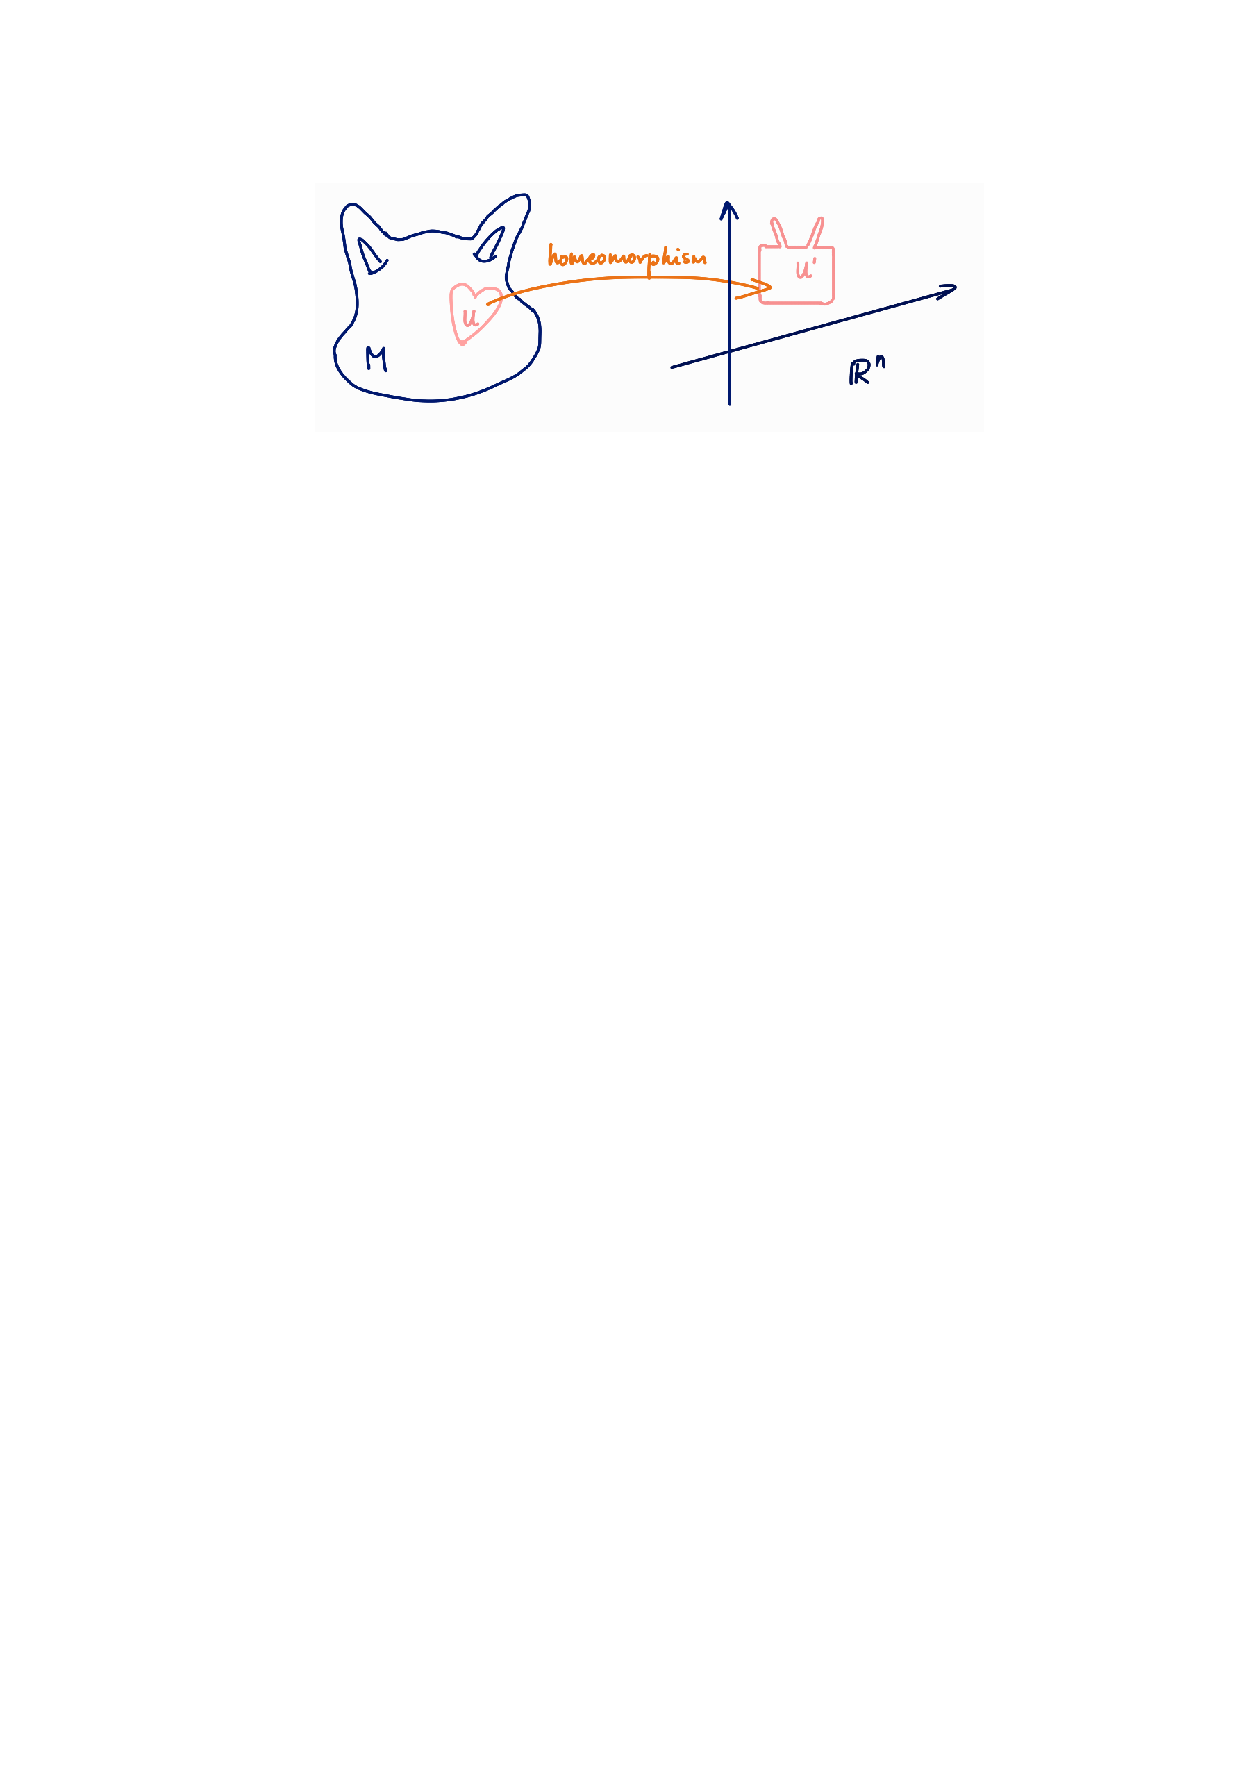
\includegraphics[scale=0.69]{topoMan}
\end{center}

\begin{defn}
Let $M$ be a topological $n$-manifold. A coordinate atlas is a collection of charts $(U_\alpha, \phi_\alpha)$ such that the set $\{U_\alpha\mid \alpha \in \mathcal{J}\}$ forms an open covering of $M$, that is $M = \bigcup_{\alpha\in\mathcal{J}} U_\alpha$, with $\mathcal{J}$ being an index set, and such atlas is denoted as $\mathcal{A} = \{(U_\alpha, \phi_\alpha)\mid \alpha \in \mathcal{J} \}$. The atlas $\mathcal{A}$ is said to be locally finite provided that each point $p \in M$ is contained in only a finite collection of open sets $U_\alpha$. 
\end{defn}


\note
Let $\mathcal{A}$ be a coordinate atlas for a topological $n$-manifold $M$, let $(U_1,\phi_1)$ and $(U_2,\phi_2)$ be elements in $\mathcal{A}$. The map $\phi_2 \circ \phi_1^{-1}: \phi_1(U_1\cap U_2) \to \phi_2(U_1 \cap U_2)$ is a homeomorphism between two open subsets of the Euclidean space $\R^n$, and here $\phi_2 \circ \phi_1^{-1}$ is called a coordinate transition function, or chart transition, for the pair $(U_1,\phi_1)$ and $(U_2,\phi_2)$.
\begin{center}
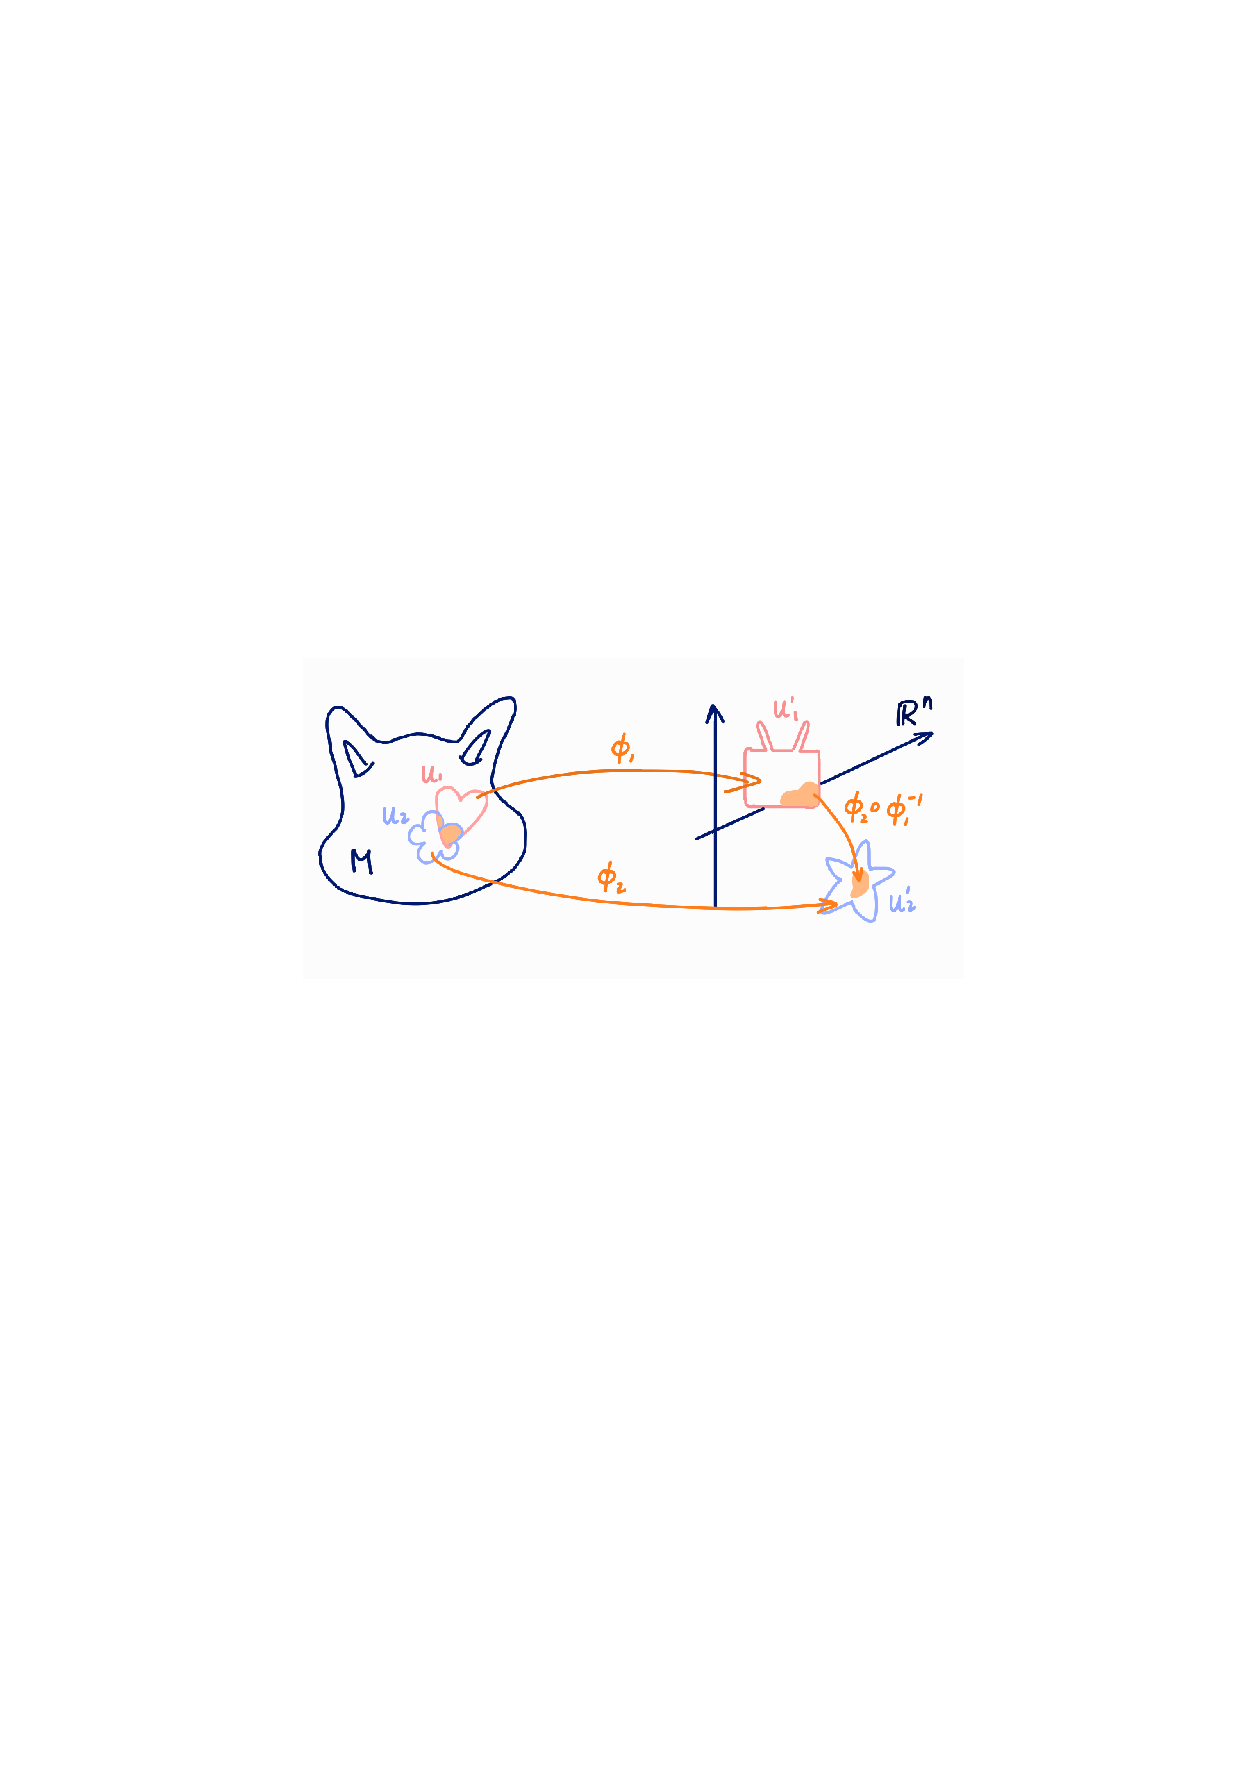
\includegraphics[scale=0.69]{transitions}
\end{center}


\begin{defn}
The atlas $\mathcal{A}= \{(U_\alpha, \phi_\alpha)\mid \alpha \in \mathcal{J}\}$ of a manifold $M$ is said to be differentiable if all coordinate transitions are differentiable. 
\end{defn}


\begin{defn}
A smooth structure on a topological $n$-manifold $M$, or the differentiable structure on $M$ is defined by an equivalence class $\mathbb{A} = [\mathcal{A}]$ of differentiable coordinate atlases. The coordinate atlases $\mathcal{A}_1$ and $\mathcal{A}_2$ for $M$ are said to be equivalent provided that, for $(U_1,\phi_1) \in \mathcal{A}_1$ and $(U_2,\phi_2) \in \mathcal{A}_2$, the compositions $\phi_1 \circ \phi_2^{-1}: \phi_2(U_1 \cap U_2) \to \phi_1(U_1 \cap U_2)$ and $\phi_2 \circ \phi_1^{-1}: \phi_1(U_1 \cap U_2) \to \phi_2(U_1 \cap U_2)$ are diffeomorphisms between subsets of Euclidean spaces. For convention and technical reasons, the smooth structure of $M$ usually refers to the maximal atlas in $\mathbb{A}$. 
\end{defn}

\begin{defn}
A manifold $M$ equipped with a smooth structure is called a smooth manifold, or a differentiable manifold. 
\end{defn}


\remark The collection of continuously differentiable functions from a topological $n$-manifold $M$ to $\R$ is denoted as $C^k(M,\R)$. Here $C^\infty(M,\R)$ consists of functions $f$ with the property as follows: Let $\mathcal{A}$ be any given atlas from the equivalence class that defines the smooth structure of a topological $n$-manifold $M$. If $(U_1,\phi_1) \in \mathcal{A}$, then $f\circ \phi_1^{-1}$ is a smooth function on $\R^n$. This defines the same set of smooth function no matter the choice of representitive atlas by virtue of Definition 1.0.0.0.4 which defines the equivalence relations. \\



\subsection{The Grassmannians}
The Grassmann manifolds, or the Grassmannians, denoted as $\text{Gr}(n,m)$, with $m,n\in \N$, are defined by the following:
\begin{align*}
\text{Gr}(n,m)\coloneqq \{ \text{all }n\text{-dimensional subspaces of }\R^{m+n}\}
\end{align*}
First we note that $\text{Gr}(m,n)$ has the structure of an $mn$-dimensional manifold. Here $\text{Gr}(1,m)$ is $\R P^m$, and $\text{Gr}(0,m), \text{Gr}(n,0)$ are single-element sets. We can obtain structure of a smooth manifold by exhibiting a coordinate atlas whose transition functions are diffeomorphism. First one can equip $\text{Gr}(n,m)$ with a suitable metrizable topology. \\

Let $\Pi \in \text{Gr}(n,m)$, and let $\mathcal{L}(\Pi, \Pi^\perp)$ denote the $mn$-dimensional space of linear maps from $\Pi$ to $\Pi^{\perp}$. Here we define: 
$$\varphi_{\Pi}:\mathcal{L}(\Pi, \Pi^{\perp}) \to \text{Gr}(n,m) \qquad \alpha\mapsto\left( \mathbb{I}\oplus \alpha\right) (\Pi)
$$
where $\mathbb{I}\oplus \alpha$ is regarded as a map from $\Pi$ to $\Pi\oplus \Pi^{\perp} = \R^{n+m}$ with $\mathbb{I}$ as the identity map:
\begin{align*}
\mathbb{I}\oplus \alpha : \Pi \to \Pi \oplus \Pi^{\perp} \qquad v\mapsto v+\alpha(v)
\end{align*}
That is, $\varphi_{\Pi}(\alpha)$ is the graph of $\alpha$ in $\Pi \oplus \Pi^{\perp} = \R^{n+m}$. It is obvious that $\varphi_{\Pi}$ is injective, thus $(\mathcal{L}(\Pi, \Pi^{\perp}), \varphi_{\Pi})$ constitutes an $mn$-dimensional chart of $\text{Gr}(n,m)$ under a slight modification of the codomain of $\varphi_{\Pi}$. The images $\varphi_{\Pi}(\mathcal{L}(\Pi, \Pi^{\perp}))$ covers $\text{Gr}(n,m)$ because here we have $\Pi = \varphi_{\Pi}(0) \in \varphi_{\Pi}(\mathcal{L}(\Pi, \Pi^{\perp}))$. \\
\begin{center}
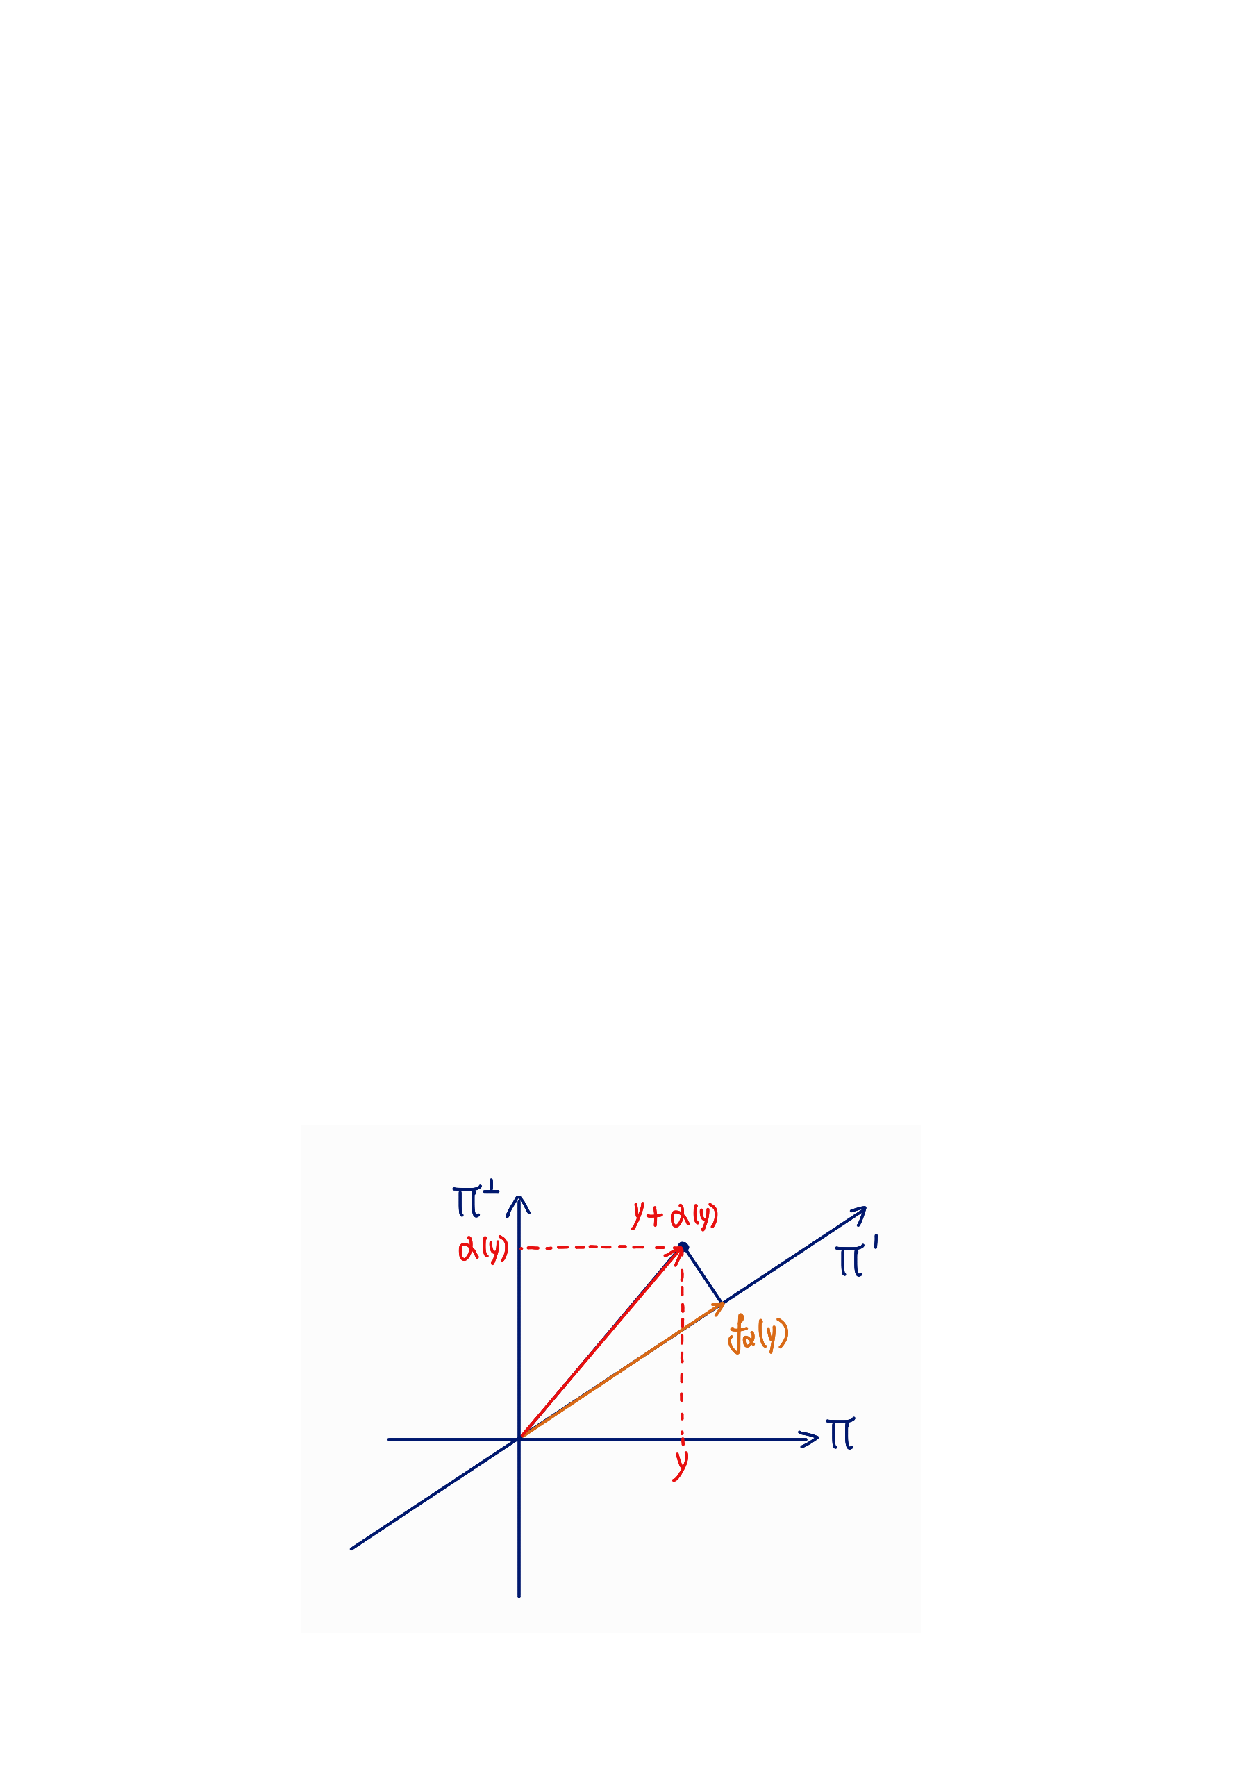
\includegraphics[scale=0.69]{GR}
\end{center}
These charts $(\mathcal{L}(\Pi, \Pi^{\perp}), \varphi_{\Pi})$  are mutually compatible. Let $\Pi, \Pi' \in \text{Gr}(n,m)$ and let $p$ and $p'$ be orthogonal projections from $\R^{m+n}$ onto $\Pi$ and $\Pi'$, respectively. Consider the map:
\begin{align*}
F = \varphi_{\Pi'}^{-1}\circ \varphi_{\Pi} : \varphi_{\Pi}^{-1}\left( \varphi_{\Pi'}\left( \mathcal{L}\left(\Pi', \left(\Pi'\right)^{\perp}\right)\right)\right) \to \varphi_{\Pi'}^{-1}\left( \varphi_{\Pi}\left(\mathcal{L}\left(\Pi, \Pi^{\perp}\right) \right)\right)
\end{align*}
Here we need check that $F$ is smooth. Note that, for $\alpha \in \varphi_{\Pi}^{-1}( \varphi_{\Pi'}( \mathcal{L}(\Pi', (\Pi')^{\perp})))$, and $\beta \in \varphi_{\Pi'}^{-1}( \varphi_{\Pi}(\mathcal{L}(\Pi, \Pi^{\perp}) ))$, we have $F(\alpha) = \beta$ if and only if we have $\varphi_{\Pi}(\alpha) = \varphi_{\Pi'}(\beta)$. We will find an analytic expression for $F(\alpha)$ by using the following construction. Let $\mathbb{I}_{X}$ denote the identity function on the linear space $X$. Here we define $f_\alpha : \Pi \to \Pi'$:
\begin{align*}
f_\alpha = p'\circ \left(\mathbb{I}_{\Pi} \oplus \alpha\right)
\end{align*}
We are only interested in the situation where we can write $F(\alpha) = \beta$ for some $\beta$, hence we can put more restriction on the definition of domain and codomain of $f_\alpha$. Here for all $y \in \Pi$, we should have the following hold if $F(\alpha) = \beta$:
\begin{align*}
y+\alpha(y) = f_\alpha (y) + \beta (f_\alpha(y))
\end{align*}
then one can show that $f_\alpha$ is invertible. Note that the condition $\det(f_\alpha) \neq 0$ already gives an exact description of the subset $\varphi_{\Pi}^{-1}(\varphi_{\Pi'}(\mathcal{L}(\Pi', (\Pi')^{\perp}))$ of $\mathcal{L}(\Pi, \Pi^{\perp})$, which is therefore open. Moreover, here we have $(\mathbb{I}_{\Pi'}\oplus \beta)\circ f_\alpha = \mathbb{I}_{\Pi}\oplus \alpha$. That is, we can write:
$$F(\alpha) = \beta = (\mathbb{I}_{\Pi}\oplus \alpha) \circ f_\alpha^{-1} - \mathbb{I}_{\Pi'}$$ Then by such construction, we see that $F$ is indeed smooth.\\

Hence we obtain for $\text{Gr}(n,m)$ an infinite atlas with charts labeled by $\Pi\in \text{Gr}(n,m)$. It suffices to consider only $\binom{n+m}{n}$ charts corresponding to subspaces $\Pi$ spanned with $n$ coordinate axes. \\


\subsection{Orientation of Manifolds}
\begin{defn}
An atlas for a differentiable manifold is said to be oriented provided that all chart transitions have positive functional determinant.
\end{defn}

\begin{defn}
An differentiable manifold is said to be orientable if it possesses an oriented atlas.
\end{defn}

\begin{defn}
Let $M$ be an orientable manifold. An oriented differentiable structure is called an orientation of $M$. $M$ equipped with an oreintation is said to be oriented. 
\end{defn}

\note Two oriented differentiable structures of a differentiable manifold determine the same orientation if the union of the two is also oriented. \\

\remark If $M$ is orientable and connected, then there exists exactly two distinct orientation on $M$.\\

\example $S^n \subseteq \R^{n+1}$ is an $n$-manifold, where we define:
$$S^n= \left\{(x_1,x_2,\cdots, x_{n+1}) \in \R^{n+1} \mid \sum_{i=1}^{n+1} x_i^2 = 1\right\}$$ 
For open subsets of $S^n$:
$$U_i^+ \coloneqq \{ (x_1,x_2,\cdots, x_{n+1})\in S^n \mid x_i >0\}\qquad\quad U_i^- = \{ (x_1,x_2,\cdots, x_{n+1}) \in S^n \mid x_i < 0 \}$$ 
we can define charts $h_i^{\pm}: U^{\pm}_i \to \R^n \ \ \ (x_1,x_2,\cdots, x_{n+1}) \mapsto (x_1,x_2,\cdots, \hat{x}_i , \cdots x_{n+1})$. \\

\begin{defn}
Let $M$ and $N$ be smooth manifolds, let $\mathcal{U}$ be a locally finite atlas from the equivalent class that gives the smooth structure on $M$, and let $\mathcal{V}$ be a locally finite atlas from the equivalent class that gives the smooth structure on $N$. A map $h:M \to N$ is said to be smooth provided that each map between Euclidean spaces in the following collection is of $C^\infty$ type:
$$\{\psi \circ h \circ \phi^{-1} \mid h(U)\cap V \neq \emptyset, \ \text{for some }(U,\phi) \in \mathcal{U},\ (V,\psi)\in \mathcal{V}\}$$
\end{defn}

\remark The equivalent relation of atlases defined in Definition 1.0.0.0.4 guarantees the definition of smooth map depends only on the smooth structure of $M$ and $N$, but not on the chosen representative coordinates. 

\begin{defn}
Two smooth manifolds are said to be diffeomorphic to each other provided that there exists a smooth homeomorphism $h:M \to N$ with smooth inverse. 
\end{defn}

\exercise Let $M_1$ and $M_2$ be differentiable manifolds, and let $\phi: M_1 \to M_2$ be a diffeomorphism, one can check that the followings hold:
\begin{enumerate}[topsep=3pt,itemsep=-1ex,partopsep=1ex,parsep=1ex]
\item $M_1$ is orientable if and only if $M_2$ is orientable.
\item If $M_1$ and $M_2$ are both connected and oriented, then $\phi$ induces an orientation on $M_2$ that may or may not coincide with the initial orientation of $M_2$. If the two orientations coincide, we say that $\phi$ is orientation preserving, and if the two orientations do not coincide, we say that $\phi$ is orientation reversing. 
\end{enumerate}


\begin{defn}
A closed manifold is a manifold without boundary that is compact.
\end{defn}
\begin{defn}
An open manifold is a manifold without boundary that has only non-compact components. 
\end{defn}

\example The circle is the only $1$-dimensional connected closed manifold. \\
\example A line without endpoint is an example of open manifold. \\

\example If $M$ can be covered by two coordinate neighborhoods $V_1$ and $V_2$ such that $V_1 \cap V_2$ is connected, then $M$ is orientable. The determinant of differentiable transition is nonzero, which implies the determinant does not change sign in $V_1 \cap V_2$.\\

\example Consider the $S^n$ ball:
\begin{align*}
S^n \coloneqq \left\{ (x_1,x_2,\cdots, x_{n+1}) \in \R^{n+1}\mid \sum_{i=1}^{n+1}x_i^2  = 1\right\} \subseteq \R^{n+1}
\end{align*}
we want to show that $S^n$ is orientable. Here we define $\Pi_1$ and $\Pi_2$ as the followings:
\begin{align*}
&\Pi_1 : S^n \setminus \{N\} \to \R^n \qquad (x_1,x_2,\cdots,x_{n+1}) \mapsto \left( \frac{x_1}{1-x_{n+1}} , \frac{x_2}{1-x_{n+1}},\cdots, \frac{x_n}{1-x_{n+1}}\right)\\
&\Pi_2 : S^n \setminus \{S\} \to \R^n \qquad (x_1,x_2,\cdots,x_{n+1}) \mapsto \left( \frac{x_1}{1+x_{n+1}} , \frac{x_2}{1+x_{n+1}},\cdots, \frac{x_n}{1+x_{n+1}}\right)
\end{align*}
where $S$ is the south pole of $S^n$ and $N$ is the north pole of $S^n$. Both $\Pi_1$ annd $\Pi_2$ are differentiable and injective, they map their domain onto the hyperplane $x_{n+1} = 0$. The two parametrizations $(\R^n, \Pi^{-1}_1)$ and $(\R^n, \Pi_2^{-1})$  cover $S^n$. Consider the change of coordinate defined by the following, with $(y_1,y_2,\cdots, y_n) \in \R^n$:
\begin{align*}
y_j = \frac{x_j}{1-x_{n+1}}\qquad\qquad\qquad y_j' = \frac{x_j}{1+x_{n+1}} = \frac{y_j}{\sum_{i=1}^n y_i^2}
\end{align*}

Here $\Pi_{1}^{-1}(\R^n) \cap \Pi_2^{-1}(\R^n)  = S^n \setminus \{N, S\}$ is connected. Hence we see that $S^n$ is orientable. Consider $A:S^n \to S^n\ \ \ p\mapsto-p$. Clearly, we see here $A$ is differentiable, and we have $A^2=\mathbb{I}$. Hence $A$ is a diffeomorphism of $S^n$. In particular, one can check that $A$ is orientation reversing if $n$ is even, and $A$ is orientation preserving if $n$ is odd.\\

\example The Grassmannians $\text{Gr}(k,n)$ is orientation if and only if $n$ is even or $n = 1$. However, the complex Grassmannians $\text{Gr}_{\C}(k,n)$ are all orientable.\\

\subsection{Complex Manifolds}
\begin{defn}
A complex manifold of complex dimension $d$ is a differentiable manifold of real dimension $2d$ whose charts have domains defined on open subsets of $\C^d$ with holomorphic charts transitions.  
\end{defn}

For notation, one can write $z \in \C^d$ as $z = (z^1,z^2,\cdots z^d)$ with $z^j = x^j+iy^j$ for some $x^j,y^j\in \R$. Here we denote $z = (x^1,x^2,\cdots,x^d,y^1,y^2,\cdots,y^d)$, and $\overline{z^{j}} = z^{\bar{j}} = x^j - iy^j$. \\

For charts $(U_\alpha, z_\alpha)$ and $(U_\beta, z_\beta)$ on a complex manifold, the transition function for the two charts is defined by:
$$z_\beta \circ z_\alpha^{-1}:z_\alpha(U_\alpha \cap U_\beta) \to z_\beta(U_\alpha \cap U_\beta)$$ 
and it is required that $z_\beta \circ z_\alpha^{-1}$ to be holomorphic, that is we can write:
\begin{align*}
\frac{\pd z_\beta^j}{\pd z_\alpha^{\bar{k}}} = 0\qquad\qquad \text{for all }j,k \text{ where }\frac{\pd}{\pd x^{\bar{k}}} = \frac{1}{2}\left( \frac{\pd}{\pd x^{\bar{k}}} +i \frac{\pd}{\pd y^{\bar{k}}}\right)
\end{align*}
The complex manifolds are always orientable because holomorphic map always has positive functional determinant.\\

\begin{defn}
A function $f:X\to Y$ is said to be of $C^\infty_0$-type provided that $f$ is of $C^\infty$-type and the set $\{x \in X \mid f(x) \neq 0\}$ has compact closure.
\end{defn}


\begin{lem}
Let $M$ be a differentiable manifold, and let $\mathcal{U} = \{U_\alpha\mid \alpha \in \mathcal{A}\}$ be an open covering for $M$ with some index set $\mathcal{A}$. Then there exists a partition of unity subordinate to $\mathcal{U}$. That is, there exists a locally finite refinement $\mathcal{V} = \{V_\beta\mid \beta\in \mathcal{B}\}$ of $\mathcal{U}$ and $C^\infty_0$ functions $\phi_\beta : M \to \R$ with the following properties hold: 
\begin{enumerate}[topsep=3pt,itemsep=-1ex,partopsep=1ex,parsep=1ex]
\item $\text{supp}(\phi_\beta) \subseteq V_\beta$ for all $\beta \in \mathcal{B}$
\item $0\leq \phi_\beta(x) \leq 1$ for all $x \in M$ and all $\beta \in \mathcal{B}$
\item $\sum_{\beta \in \mathcal{B}}\phi_\beta(x) = 1$ for all $x \in M$
\end{enumerate}  
Note here in (3), there are only finitely many non-vanishing summands at each point in $M$ because only finitely many $\phi_\beta$ are non-zero at any given point, as covering $\mathcal{V}$ is locally finite. 
\end{lem}

\newpage
\section[Tangent Spaces]{\color{red}Tangent Spaces\color{black}}
The following considerations motivate the notation that we use for tangent vector. Consider $\alpha:(-\epsilon,\epsilon) \to \R^n$ to be a differentiable curve in $\R^n$, with $\alpha(0) = p$ and $\epsilon>0$. Here we can write:
\begin{align*}
\alpha(t) = (x_1(t), x_2(t),\cdots, x_n(t)) \qquad\qquad t\in (-\epsilon, \epsilon), \ (x_1,x_2,\cdots, x_n) \in \R^n
\end{align*}
Then $\alpha'(0) = (x_1'(0),x_2'(0),\cdots, x_n'(0)) = v \in \R^n$ is the velocity of the curve when passing $p$. If one suppose $f$ to be a real-valued differentiable function defined in a neighborhood of $p$, we can restrict $f$ to the curve $\alpha$ and express the directional derivative with respect to the vector $v$ as the following:
\begin{align*}
\left.\frac{d}{dt}(f\circ \alpha) \right|_{t = 0} = \sum_{i=1}^n \left.\frac{\pd f}{\pd x_i}\right|_{t=0} \left.\frac{dx_i}{dt}\right|_{t=0} = \left( \sum_{i=1}^n x_i'(0) \frac{\pd}{\pd x_i}\right) f
\end{align*}  
Therefore, the direction derivative with respect to $v$ is an operator on the differentiable function $f$. Viewing $v$ as a tangent vector, one would like to denote $v$ as the form:
\begin{align*}
v =  (x^i)'(0) \frac{\pd}{\pd x^i}
\end{align*}


\begin{defn}
Consider $\R^d$, and let $x = (x^1,x^2,\cdots, x^d)$ be Euclidean coordinates of $\R^d$, let $\Omega \subseteq \R^d$ be an open set, and let $x_0 \in \Omega$. The tangent space of $\Omega$ at the point $x_0$ is denoted as $T_{x_0}\Omega$, and is defined by the space $\{x_0\}\times E$, where $E$ is the $d$-dimensional Euclidean space spanned by the basis $\{ \pd/\pd x^1, \pd/\pd x^2, \cdots, \pd/\pd x^d\}$.\footnote{Here $\pd/\pd x^i$ is identified as the standard basis element $e_i \in \R^d$} Moreover, for open subset $\Omega$ of $\R^d$, $T\Omega \coloneqq \Omega \times E $.
\end{defn}

\begin{defn}
Let $\Omega,\Omega' \subseteq \R^d$ be open sets, and that $f:\Omega \to \Omega'$ defines a diffeomorphism. Here $df(x_0)$ for $x_0 \in \Omega$ induces a linear map between the tangent spaces $T_{x_0}\Omega$ and $T_{f(x_0)}\Omega'$:
\begin{align*}
F(x_0): T_{x_0}\Omega \to T_{f(x_0)}\Omega' \qquad \left(x_0,\ v^i \frac{\pd}{\pd x^i}\right)\mapsto \left(f(x_0),\ v^i \left.\frac{\pd f^j}{\pd x^i}\right|_{x_0} \frac{\pd }{\pd f^j}\right)
\end{align*}
where we have:
\begin{align*}
df(x_0): \R^d \to \R^d \qquad v^i \frac{\pd}{\pd x^i}\mapsto v^i \left.\frac{\pd f^j}{\pd x^i}\right|_{x_0} \frac{\pd }{\pd f^j}
\end{align*}
\end{defn}

\note For open set $\Omega \subseteq \R^d$, $T\Omega = \Omega \times E\cong \Omega \times \R^d$. One can view $T\Omega$ as an open subset of $\R^d \times \R^d$, and is a differentiable manifold itself.  
$$\Pi: T\Omega \to \Omega \ \ \ (x,v)\mapsto x$$ 
Here $\Pi$ is the natural projection from $T\Omega$ to $\Omega$, and the triple $(T\Omega,\Pi, \Omega)$ is called a tangent bundle of $\Omega$ and $T\Omega$ is called the total space of the tangent bundle. In such case, if $\Omega'\subseteq \R^d$ is an open set and $f:\Omega\to \Omega'$ defines a diffeomorphism, then the induced linear map between $T\Omega$ and $T\Omega'$ is of the form similar to $df$:
\begin{align*}
F: T\Omega \to T\Omega' \qquad \left(x,\ v^i\frac{\pd}{\pd x^i}\right)\mapsto \left( f(x),\  v^i \left.\frac{\pd f^j}{\pd x^i}\right|_{x}\frac{\pd}{\pd f^j}\right)
\end{align*}
In particular, if $g:\Omega \to \R$ is a differentiable function for open $\Omega \subseteq \R^n$ and $v = v^i \frac{\pd}{\pd x^i}$, then we can write the following for $x \in \Omega$:
\begin{align*}
dg(x)(v) =v^i \left.\frac{\pd g}{\pd x^i}\right|_x
\end{align*}

When $(U,x)$ is denoted as a chart for a manifold $M$ of dimension $d$, then we know that $x:U \to \R^d$ is a diffeomorphism. For $p \in M$, $x(p) = (x^1(p),x^2(p),\cdots, x^d(p))$. $x(p)$ is called the local coordinate of $p$. Hence a local coordinate on $U$ is usually denoted as $(x^1,x^2,\cdots, x^d)$. We will see later that such chart induces a natural basis for the tangent space of $M$ at $p$, denoted as $T_pM$. In this case, we shall identify $\{\pd/\pd x^i\mid 1\leq i \leq d\}$ as the set of basis elements of $T_pM$, where we define $\pd/\pd x^i$ to be the $i$-th column of the Jacobian matrix $dx^{-1}(x(p))$. For $v\in \R^d$, we identify $\pd/\pd x^i$ as the usual standard basis element $e_i$. In the following discussion, the base point of a tangent vector is usually omitted, that is, for $v \in T_z\Omega$ for some $z \in \R^d$ and open set $\Omega \subseteq \R^d$, we denote $v$ as the following:
\begin{align*}
v = v^i \frac{\pd}{\pd x^i}
\end{align*}

Now let $M$ be a differentiable manifold of dimension $d$, and let $p \in M$. We will consider the criteria to define a tangent space of $M$ at point $p$. Let $x: U \to \R^d$ be a chart for $M$ with $p \in U$, and $U \subseteq M$ is open. Let $x':U'\to \R^d$ be another chart for $M$ with $p \in U'$ and $U'$ being open in $M$. The tangent space $T_pM$ can now be represented in the chart $(U,x)$ by $T_{x(p)}x(U)$, and represented in the chart $(U',x')$ by $T_{x'(p)}x'(U')$. We denote $\Omega = x(U)$, $\Omega' = x'(U')$, and consider transition map:
\begin{align*}
x' \circ x^{-1} : x(U \cap U') \to x'(U \cap U') 
\end{align*}
where we see that $x' \circ x^{-1}$ induces a vector space isomorphism:
\begin{align*}
L\coloneqq d(x'\circ x^{-1}) (x(p)) : T_{x(p)}\Omega \to T_{x'(p)}\Omega'
\end{align*}
For $v \in T_{x(p)}\Omega$ and $L(v) \in T_{x'(p)}\Omega'$, they should represent the same tangent vector in $T_pM$, that is, a tangent vector in $T_pM$ is given by a family of coordinate representors. \\

Now consider $f:M \to \R$ to be a differentiable function. Assume that the tangent vector $w \in T_pM$ is represented by $v \in T_{x(p)}x(U)$, we want to define $df(p)$ as a linear map from $T_pM$ to $\R$. In this sense, in chart $(U,x)$ that satisfies $p \in U\subseteq M$, let $w \in T_pM$ be represented as the following: 
$$v = v^i \frac{\pd}{\pd x^i} \in T_{x(p)}x(U)$$ 
Then we should let $df(p)(w)$ in this chart be represented by $d(f\circ x^{-1})(x(p)) (v)$. \\


\remark For a $d$-dimensional manifold $M$, $T_pM$ is a vector space of dimension $d$ that is isomorphic to $\R^d$, the isomorphism between $T_pM$ and $\R^d$ depends on the choice of chart. For function on $M$, one can pull it back by a chart to an open subset of $\R^d$ and make differentiation. In order to obtain object not dependent on the chart, we have to know transformation behavior under chart changes, as we will discuss next.\\

\begin{center}
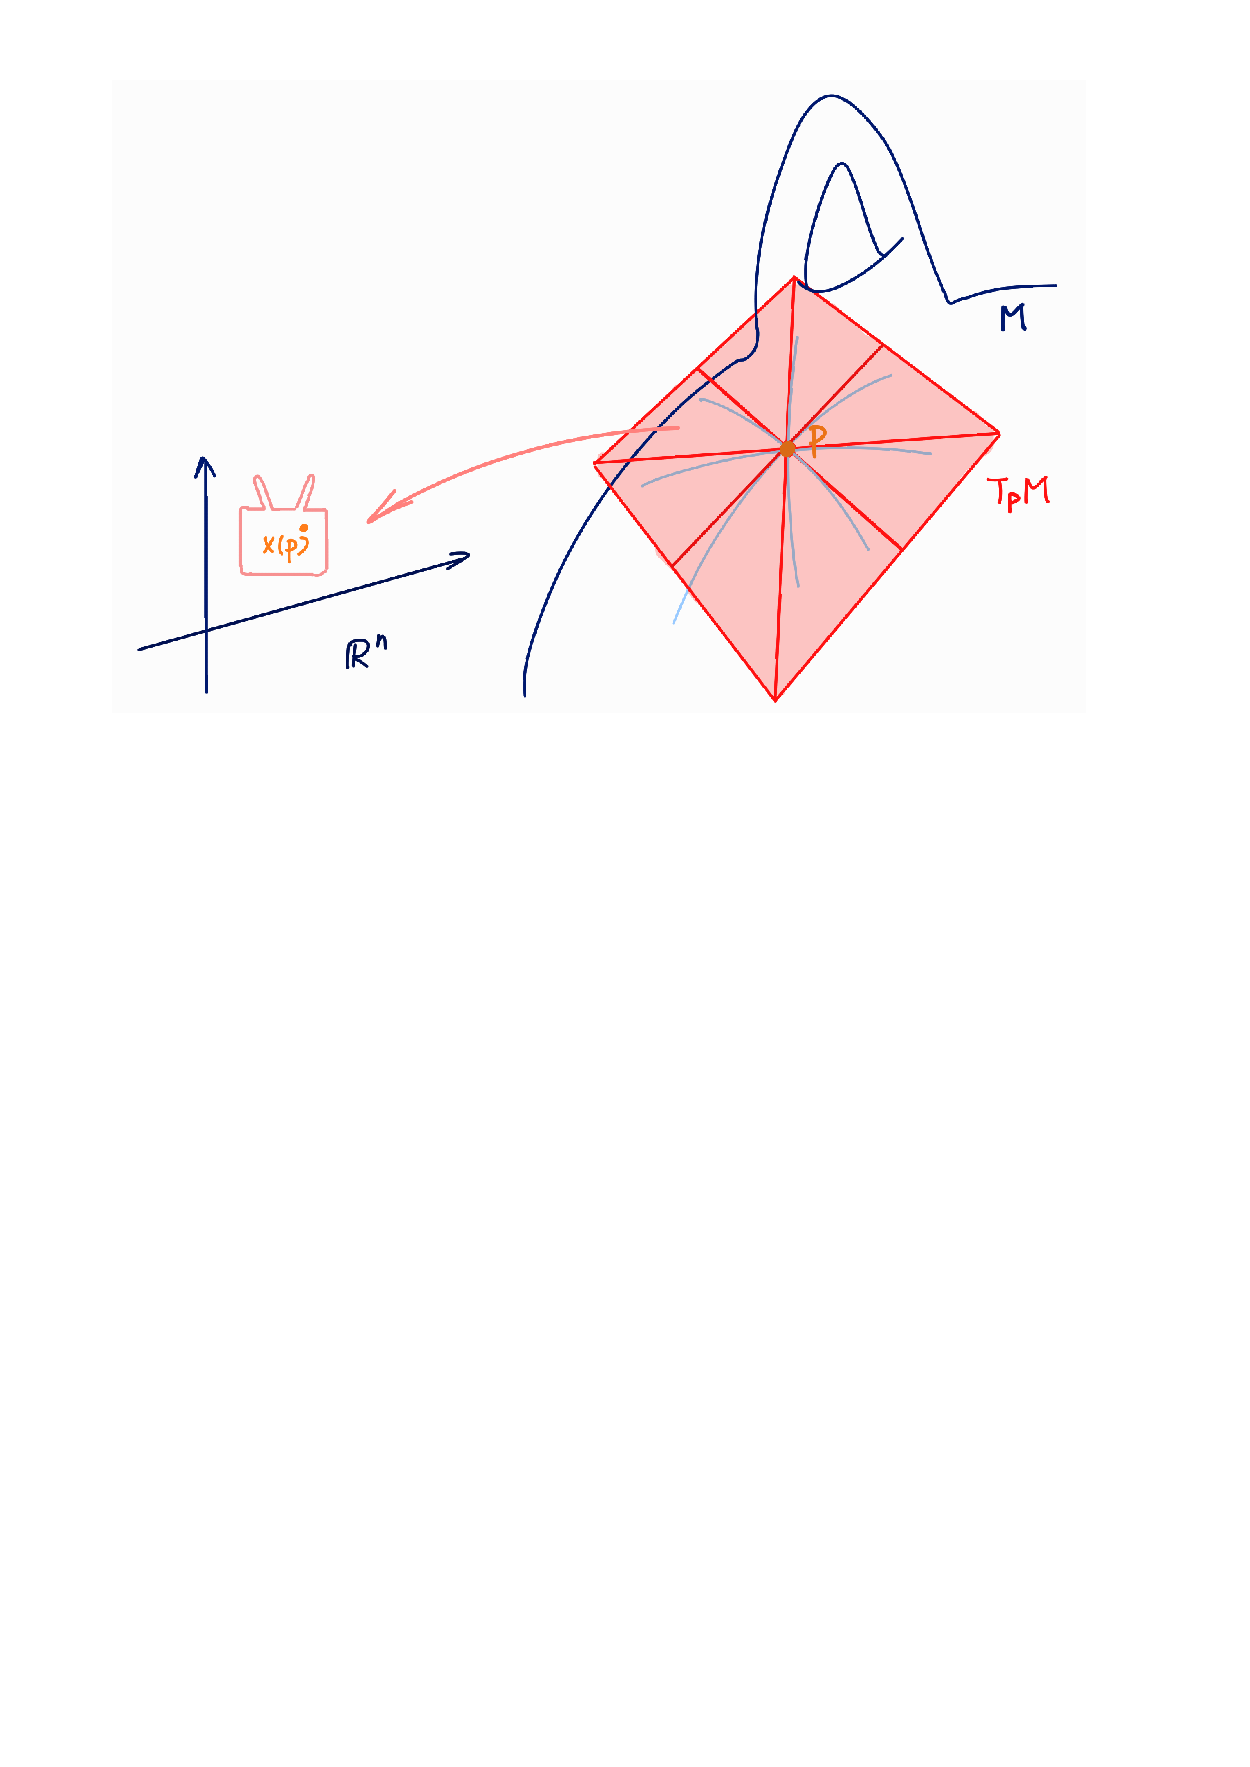
\includegraphics[scale=0.69]{tangentPlane}
\end{center}


\begin{defn}
Let $M$ be a differentiable manifold, let $p\in M$, and consider the set: 
$$\mathcal{Z}_p = \{(x,v)_p\mid x : U \to \Omega \text{ is a chart with }p \in U,\ v\in T_{x(p)}\Omega\}$$
For $(x,v)_p,(y,w)_p \in \mathcal{Z}_p$, we write $(x,v)_p \sim(y,w)_p$ provided that $w = d(y\circ x^{-1})(x(p))v$. The space of equivalent classes defined using such equivalence relation is called the tangent space at point $p$ to $M$, denoted as $T_p M$.  
\end{defn}

\note For a differentiable $d$-dimensional manifold $M$ and $p \in M$, the tangent space $T_pM$ naturally carries the structure of a vector space. Since coordinate chart $x:U \to \R^d$ for $M$ is a local diffeomorphism, that is $dx(p):U \to \R^d$ is a invertible for all $p \in M$. For $(x,v)_p,(y,w)_p \in \mathcal{Z}_p$, we write $(x,v)_p \sim(y,w)_p$ provided that $w = d(y\circ x^{-1})(x(p))v$, then it follows that:
\begin{align*}
w =\left( dy(p) \circ dx^{-1}(x(p)) \right)\, v\qquad \Rightarrow \qquad dy^{-1}(y(p)) \, w = dx^{-1}(x(p)) \, v
\end{align*}
Hence we see here the columns of $d x^{-1}(x(p))$ form a basis of $T_pM$.  


\begin{defn}
Let $M$ be a differentiable manifold. $TM$ is defined to be the disjoint union of the tangent spaces of $M$, that is, we write:
$$TM \coloneqq  \bigsqcup_{p \in M}T_pM$$ 
$\Pi:TM \to M \ \ \ [(x,v)_p]\mapsto p$ for $(x,v)_p \in \mathcal{Z}_p$ is the natural projection from $TM$ to $M$. 
\end{defn}

For a differentiable manifold $M$, if $x: U \to \R^d$ is a chart for $M$, we denote: 
$$TU \coloneqq \bigsqcup_{p\in U}T_p M$$ 
and we can write:
$$dx:TU \to Tx(U) \qquad w\mapsto dx(\Pi(w))v$$
where $v$ denote the vector associated to $w = [(x,v)_p] \in TU$. \\

\begin{defn}
For a differentiable manifold $M$. The triple $(TM, \Pi, M)$ is called a tangent bundle of $M$, and $TM$ is called the total space of the tangent bundle of $M$. 
\end{defn} 


\begin{defn}
A vector field $X$ on a differentiable manifold $M$ is defined by associating each point $p \in M$ with a vector $X(p) \in T_pM$. That is, $X$ is a mapping $X:M \to TM$. The vector filed $X$ is differentiable provided that $X: M \to TM$ is differentiable.   
\end{defn}


Let $F:M \to N$ be a differentiable map between differentiable manifold $M$ of dimension $d$ and differentiable manifold $N$ of dimension $c$.  $F$  here can be represented in local charts $x:U \to \R^d$ and $y:V\to \R^c$, by $y \circ F \circ x^{-1}$, where $U \subseteq M$ is open, and $V\subseteq N$ is open. Let the local coordinates on $U$ be denoted by $(x^1, x^2,\cdots, x^d)$, let component functions of $y\circ F$ be denoted as $(F^1, F^2,\cdots, F^c)$, then each point in $F(U)$ has local coordinate represented as follows:
$$(F^1(x^1,x^2,\cdots, x^d), F^2(x^1,x^2,\cdots, x^d),\cdots, F^c(x^1,x^2,\cdots, x^d) )$$
For $p \in U$, $dF$ now induces the linear map $dF(p):T_{p}M \to T_{F(p)}N $ which in our coordinate representation is given by a matrix: \footnote{Here $\pd F/\pd x$ is understood to be }
\begin{align*}
\left(\frac{\pd F^\alpha}{\pd x^i} \right)_{\substack{i \in \{1,2,\cdots,c\}\\ 
\alpha \in \{1,2,\cdots, d\}}}
\end{align*}
A change of charts leave to some base change of the tangent spaces, and the transformation behavior is determined by the chain rule. If the local change of chart on $M$ is given by $(x^1, x^2,\cdots, x^d)\mapsto (\xi^1,\xi^2,\cdots, \xi^d)$ and the local change of chart on $N$ is given by $(F^1,F^2,\cdots, F^c)\mapsto (\Phi^1,\Phi^2,\cdots, \Phi^c)$, then the representation of $dF$ in the new coordinates is given as the following:
\begin{align*}
\left(\frac{\pd \Phi^\beta}{\pd \xi^j} \right) = \left( \frac{\pd \Phi^\beta}{\pd F^\alpha}\frac{\pd F^\alpha}{\pd x^i}\frac{\pd x^i}{\pd \xi^j}\right)
\end{align*}



\newpage
\section[Immersions and Embeddings]{\color{red}Immersion and Embeddings\color{black}}
\begin{defn}
Let $M$ be a differentiable $m$-manifold, and $N$ be a differentiable $n$-manifold. A differentiable mapping $\varphi: M \to N$ is called an immersion provided that $d\varphi_p: T_pM  \to T_{\varphi(p)}N$ is injective for all $p \in M$. $\varphi$ is called an embedding provided that $\varphi$ is an immersion and a homeomorphism onto $\varphi(M) \subseteq N$ with $\varphi(M)$ being equipped with the subspace topology inherits from $N$. If $M \subseteq N$ and the inclusion $i:M \to N$ is an embedding, then $M$ is called a submanifold of $N$.
\end{defn}


\begin{thm}[Local Immersion Theorem]
Let $M,N$ be differentiable manifolds with $\dim(M) = m$ and $\dim(N) = n$, let $f:M \to N$ be an immersion, let $x \in M$. There exists a neighborhood $U$ of $x$ and a chart $(V,y)$ on $N$ with $f(x) \in V$ such that the followings hold:
\begin{enumerate}[topsep=3pt,itemsep=-1ex,partopsep=1ex,parsep=1ex]
\item $f|_U$ is a differentiable embedding.
\item $y^{m+1}(p) =y^{m+2}(p)= \cdots = y^n(p) = 0$ for all $p \in f(U) \cap V$.
\end{enumerate}
\end{thm}
\begin{proof}
Here we will use implicit function theorem. In local coordinates, we can choose $z = (z^1,z^2,\cdots, z^n)$ on $N$ and $x=(x^1, x^2,\cdots, x^m)$ on $M$. WLOG, since $df(x)$ is injective, we let the following matrix be non-singular:
\begin{align*}
\left(\left.\frac{\pd z^\alpha }{\pd x^i} \right|_{f(x)}\right)_{\substack{i,\alpha\in\{ 1,2\cdots, m\}}}
\end{align*}
Consider the function $F(z,x)$ defined by:
$$F(z,x) \coloneqq (z^1 - f^1(x) ,z^2 - f^2(x)  \cdots, z^n-f^n(x))$$
Note $DF(z,x)$ has maximal rank in the coordinate $(x^1, x^2,\cdots, x^m, z^{m+1},z^{m+2}, \cdots , z^n)$. By the Implicit Function Theorem, locally there exists a map $\varphi$ defined by:
$$(z^1,z^2 \cdots, z^n)\mapsto (\varphi^1(z^1,z^2\cdots, z^m),\varphi^2(z^1,z^2\cdots, z^m),\cdots, \varphi^n(z^1,z^2, \cdots, z^m))$$
with $F(z,x) = 0$ if and only if the following holds locally:
$$x^1 = \varphi^1(z^1,z^2 \cdots, z^m),\ x^2 = \varphi^2(z^1,z^2 \cdots, z^m),\ \cdots,\ x^m = \varphi^m(z^1,z^2\cdots, z^m)$$ 
$$z^{m+1} = \varphi^{m+1}(z^1,z^2 \cdots, z^m),\ z^{m+1} = \varphi^{m+2}(z^1,z^2 \cdots, z^m),\cdots,\ z^n = \varphi^n(z^1,z^2\cdots, z^m)$$ 
and the following matrix has maximal rank:
$$\left( \frac{\pd \varphi^i}{\pd z^\alpha}\right)_{\alpha, i \in\{ 1,2,\cdots, m\}}$$ 
Now we can define new coordinate $y$ as the following:
$$(y^1, \cdots, y^n) = (\varphi^1,\varphi^2,\cdots, \varphi^m, z^{m+1}-\varphi^{m+1},\cdots, z^n - \varphi^n)$$
Combing we see here $z = f(x)$ if and only if $F(z,x) = 0$, if and only if we have:
$$(y^1, \cdots, y^n) = (x^1,\cdots, x^m,0,\cdots, 0)$$
and the result of the theorem follows.
\end{proof}
\remark Theorem 3.1 shows that any immersion is locally a differentiable embedding.


\begin{lem}
Let $M,N$ be differentiable manifolds with $\dim(M) = m$ and $\dim(N) = n$, $m\geq n$,  let $p \in N$, and let $f:M \to N$ be a differentiable map with $df(x)$ having rank $n$ for all $x \in M$ that satisfies $f(x) = p$, then $f^{-1}(p)$ is the union of differentiable submanifolds of $M$ of dimension $m-n$.  
\end{lem}
\begin{proof}
The proof also makes use of the Implicit Function Theorem. 
\end{proof}

\begin{corT}
Let $N$ be a differentiable manifold, let $M\subseteq N$ be a differentiable submanifold of $N$, let $i : M \to N:  \ \ \ x\mapsto x$ be the inclusion function. Then for $p \in M$, $T_pM$ can be considered as a subspace of $T_pN \cong di(T_pM)$.
\end{corT}


\remark Let $N$ be a smooth manifold of dimension $n$, let $1\leq m\leq n$, then an arbitrary subset $M$ of $N$ has the structure of a differentiable submanifold of $N$ of dimension $m$ if and only if for all $p \in M$, there exists a $C^\infty$ chart $(U,\varphi)$ of $N$ such that for $p \in U$ that satisfy $\varphi(p) = 0$, $\varphi(U)$ is an open cube $(\epsilon, \epsilon)^n$ and $\varphi(U \cap M) = (-\epsilon, \epsilon)^m \times \{0 \}^n$.


\begin{lem}
Let $M,N$ be differentiable manifolds with $\dim(M) = m$ and $\dim(N) = n$, $m\geq n$,  let $p \in N$, and let $f:M \to N$ be a differentiable map with $df(x)$ having rank $n$ for all $x \in M$ that satisfies $f(x) = p$. For the submanifold $X = f^{-1}(p)$, and $q \in X$, we have $T_q X = \ker(df(q)) \subseteq T_q M$. 
\end{lem}

  
  
\chapter{The Geodesics}
\setcounter{section}{3}
In this chapter, we will focus on differentiable manifold that is topological connected.
\section[Riemannian Metrics]{\color{red}Riemannian Metrics\color{black}}
\begin{defn}
A Riemannian metric on a differentiable manifold $M$ is a correspondence which associates to each $p \in M$ an inner product $\langle \cdot, \cdot\rangle_p$ on the tangent space $T_pM$, and $\langle \cdot,\cdot\rangle_p$ depends smoothly on the base point $p \in M$. A Riemannian manifold is a differentiable manifold equipped with a Riemannian metric.                                                                
\end{defn}

Let $(x^1,x^2,\cdots, x^d)$ be local coordinates on a manifold $M$. Then a Riemannian metric under such coordinate is represented by a positive definite symmetric matrix:
\begin{align*}
(g_{ij}(x) ) _{i,j \in\{ 1,2,\cdots, d\}}
\end{align*}
which satisfies $g_{ij} = g_{ji}$, and $g_{ij}v^i v^j >0$ for all $v = (v^1, v^2,\cdots, v^d) \neq 0$, and that coefficients $g_{ij}$ depends smoothly on $x$. We will discuss in the following that the smoothness of such metric can be defined such that it does not depend on the choice of local coordinates, thus the smoothness dependence on the base point as required in the definition can be represented in local coordinates. \\


First we consider the product of two tangent vectors $v,w \in T_pM$ with coordinate representations $(v^1,v^2,\cdots,v^d)$ and $(w^1,w^2,\cdots, w^d)$, that is, we write:
\begin{align*}
v = v^i \frac{\pd}{\pd x^i} \qquad\qquad\qquad w = w^i \frac{\pd}{\pd x^i}
\end{align*}
Here we can write the following:
\begin{align*}
\langle v, w\rangle_p = g_{ij}(x(p))v^iw^j
\end{align*}
In particular, we have:
\begin{align*}
\left\langle \frac{\pd}{\pd x^i}, \frac{\pd}{\pd x^j}\right\rangle_p = g_{ij}(x(p))
\end{align*}
The length of $v$ here is defined to be the following:
\begin{align*}
||v|| \coloneqq \langle v, v\rangle_p^{1/2}
\end{align*}
Let $y = f(x)$ define some different local coordinates, in these, $v,w$ are represented as $(\that{v}^1, \that{v}^2,\cdots, \that{v}^d)$ and $(\that{w}^1, \that{w}^2,\cdots, \that{w}^d)$ with the followings hold:
\begin{align*}
\that{v}^j = v^i \frac{\pd f^j}{\pd x^i} \qquad\qquad\qquad \that{w}^j = w^i \frac{\pd f^j}{\pd x^i}
\end{align*}
Denote the metric in new coordinates $y$ by $h_{kl}(y)$, then we should be able to write:
\begin{align*}
h_{kl}(f(x))\that{v}^k\that{w}^l = \langle v, w\rangle_p = g_{ij}(x)v^iw^j
\end{align*}
Hence we have:
\begin{align}
h_{kl}(f(x)) \frac{\pd f^k}{\pd x^i}\frac{\pd f^l}{\pd x^j}v^iw^j = g_{ij}(x)v^iw^j
\end{align} 
(2.1) should hold for all $v,w \in T_pM$, hence the following is required to hold:
\begin{align}
h_{kl}(f(x))\frac{\pd f^k}{\pd x^i}\frac{\pd f^l}{\pd x^j} = g_{ij}(x)
\end{align}
Here (2.2) describes the transformation behavior of the representation of Riemannian metric under vector coordinate changes. \\

\example For the Euclidean space, we write:
\begin{align*}
\langle v, w\rangle = \delta_{ij} v^i w^j = v^iw^i
\end{align*}

\begin{thm}
Every differentiable manifold can be equipped with a Riemannian metric induced by the system of local coordinates. 
\end{thm}

\newpage
\section[The Euler-Langrange Equations for Energy]{\color{red}The Euler-Langrange Equations for Energy \color{black}}
\begin{defn}
Let $M$ be a differentiable manifold equipped with a Riemannian metric, let $[a,b]$ be a closed interval in $\R$, and let $\gamma[a,b] \to M$ be a smooth curve. The length of $\gamma$ is defined by the following:
\begin{align*}
\mathcal{L}(\gamma) \coloneqq \int_a^b \left\| \left.\frac{d\gamma}{dt}\right|_t \right\| \, dt
\end{align*}
The energy of $\gamma$ is defined by the following:
\begin{align*}
\mathcal{E}(\gamma) \coloneqq \frac{1}{2}\int_a^b \left\| \left.\frac{d\gamma}{dt}\right|_t \right\|^2 \, dt
\end{align*}
\end{defn}
Let $M$ be a differentiable manifold equipped with a Riemannian metric, let $[a,b]$ be a closed interval in $\R$, and let $\gamma[a,b] \to M$ be a smooth curve. We will compute $\mathcal{L}(\gamma)$ and $\mathcal{E}(\gamma)$ in local coordinates: $(x^1(\gamma(t)),x^2(\gamma(t)),\cdots, x^d(\gamma(t)))$. Here we denote:
\begin{align*}
\dot{x}^i(t) = \frac{d}{dt}\left( x^i(\gamma(t))\right)
\end{align*}
Then we can write the following:
\begin{align*}
\mathcal{L}(\gamma) &= \int_a^b \sqrt{g_{ij}(x(\gamma(t))\, \dot{x}^i(t)\, \dot{x}^j(t)} \, dt\\
\mathcal{E}(\gamma) &=\frac{1}{2} \int_a^b g_{ij}(x(\gamma(t)) \, \dot{ x}^i(t) \, \dot{x}^j(t)\, dt
\end{align*} 
We now can define the distance between two points $p,q \in M$ as the following.
\begin{defn}
Let $M$ be a differentiable manifold equipped with a Riemannian metric.
\begin{align*}
d(p,q)\coloneqq \inf\left\{ \mathcal{L}(\gamma) \mid \gamma:[a,b]\to M  \text{ is a piecewirse smooth curve with }\gamma(a) = p, \ \gamma(b) = q\right\}
\end{align*}
\end{defn}

Here we see that by equipping a differentiable manifold with a Riemannian metric, we are able to define distance between points on the manifold. 
\begin{defn}
A differentiable manifold equipped with a Riemannian metric is called a Riemannian manifold. 
\end{defn}

\begin{lem}
For a Riemannian manifold $M$, any two points $p,q \in M$ can be connected by a piecewise smooth curve, that is $d(p,q)$ always exists.
\end{lem}

\begin{corT}
Let $M$ be a Riemannian manifold, the topology of $M$ induced by the length functional defined by $\mathcal{L}$ coincides with the topology on $M$. 
\end{corT}

\begin{lem}
Let $M$ be a Riemannian manifold, if $\gamma:[a,b]\to M$ is a smooth curve, and $\psi:[\alpha,\beta] \to [a,b]$ is a parameter change, then $\mathcal{L}(\gamma\circ \psi) = \mathcal{L}(\gamma)$. That is, the length functional $\mathcal{L}$ is invariant under parameter changes. 
\end{lem}

For notation, if $(g_{ij})$ denote a positive definite matrix that defines the Riemannian metric on a manifold $M$, we then denote:
\begin{align*}
(g^{ij})_{i,j \in\{1,2,\cdots, d\}} = \left( g_{ij}\right)^{-1}_{i,j \in\{1,2,\cdots, d\}}\qquad\qquad\qquad g_{jl, k}\coloneqq \frac{\pd}{\pd x^k}g_{jl}
\end{align*}
That is, we have:
\begin{align*}
g^{il}g_{lj} = (\delta_{ij})_{i,j \in\{1,2,\cdots, d\}}
\end{align*}

Here we define the Christoffel symbols:
\begin{align*}
\Gamma_{jk}^i \coloneqq \frac{1}{2}g^{il}\left( g_{jl,k} + g_{kl,j} - g_{jk,l}\right)
\end{align*}


\begin{prop}
The Euler-Lagrange Equations for the energy $\mathcal{E}$ is given by the following:
\begin{align}
\ddot{x}^i(t) + \Gamma_{jk}^i (x(t)) \dot{x}^j(t) \dot{x}^k (t) = 0
\end{align}
\end{prop}
\begin{proof}
Let $I$ be a functional defined by the following:
\begin{align*}
I(x) = \int_a^b f(x(t), \dot{x}(t)) \, dt
\end{align*}
The Euler-Lagrange Equations of a functional $I$ is given by the following:
\begin{align*}
\frac{d}{dt}\frac{\pd f}{\pd \dot{x}^i} - \frac{\pd f}{\pd x^i} = 0\qquad\qquad \forall i \in \{1,2,\cdots, d\}
\end{align*}
Here we obtain for $\mathcal{E}$, for all $i\in \{1,2,\cdots, d\}$:
\begin{align*}
\frac{d}{dt}\left( g_{ik}(x(t)) \dot{x}^k(t) + g_{ji}(x(t)) \dot{x}^j(t) \right) - g_{jk,i}(x(t)) \dot{x}^j(t) \dot{x}^k(t) = 0
\end{align*}
Hence we get:
\begin{align*}
g_{ik}\ddot{x}^k + g_{ji}\ddot{x}^j + g_{ik,l}\dot{x}^l \dot{x}^k + g_{ji,l}\dot{x}^l \dot{x}^j -g_{jk,i}\dot{x}^j\dot{x}^k = 0
\end{align*}
Rearranging we get:
\begin{align}
2g_{lm}\ddot{x}^m + \left( g_{lk,j}+ g_{jl,k}-g_{jk,l}\right) \dot{x}^j\dot{x}^k = 0 
\end{align}
Simplifying, we have:
\begin{align*}
g^{il}g_{lm}\ddot{x}^m + \frac{1}{2}g^{il}\left( g_{lk,j}+ g_{jl,k}-g_{jk,l}\right) \dot{x}^j\dot{x}^k &= 0 \\
\ddot{x}^i + \frac{1}{2}g^{il}\left( g_{lk,j}+ g_{jl,k}-g_{jk,l}\right) \dot{x}^j\dot{x}^k &= 0
\end{align*}
This completes the proof.
\end{proof}


\begin{defn}
Let $M$ be a Riemannian manifold, a smooth curve $\gamma:[a,b]\to M$ that obeys (2.3) is called a geodesic. 
\end{defn}


Let $I$ be defined by the following:
\begin{align*}
I(\omega) = \int_0^t f(\dot{w}(s), w(s))\, ds
\end{align*}
which defined for functions $w = (w^1,w^2,\cdots, w^n)$ of the admissible class:
\begin{align*}
\mathcal{A} = \left\{ w\in C^2([0,t],\R^n) \mid w(0) = y, w(t) = x\right\}
\end{align*}
From calculus of variation, we can find a curve $w \in \mathcal{A}$ such that the following is true:
\begin{align*}
I(x) = \min_{\omega \in \mathcal{A}} I(\omega)
\end{align*}

\begin{thm}
The function $w$ that solves the system of Euler-Lagrange Equations satisfies:
\begin{align*}
-\frac{d}{ds}\left( D_{\dot{w}}f(\dot{w}(s), w(s))\right) + D_wf(\dot{w}(s),w(s)) = 0
\end{align*}
\end{thm}

\note From Definition 5.0.4.0.1, we see that a geodesic on a Riemannian manifold is a extremum of the energy function $\mathcal{E}$ defined on the manifold. A geodesic is not necessarily length minimizing, nor energy minimizing. The existence of solution to ODE (2.3) is guaranteed by the Cauchy-Lipchitz Theorem. 

\begin{prop}
Let $M$ be a Riemannian manifold. For all smooth curves $\gamma:[a,b]\to M$, we have:
\begin{align*}
\left(\mathcal{L}(\gamma)\right)^2 \leq 2(b-a)\, \mathcal{E}(\gamma)
\end{align*}
with equality if and only if $||d\gamma/df|| = \text{constant}$. 
\end{prop}
\begin{proof}
Using Holder's Inequaility, we can write the following:
\begin{align*}
\int_a^b \left\| \frac{d\gamma}{dt}\right\|\, dt \leq (b-a)^{1/2}\left( \int_a^b \left\|\frac{d\gamma}{dt}\right\|^2\, dt\right)^{1/2}
\end{align*}
with equality if and only if $d\gamma/dt$ is a constant. 
\end{proof}


\example Denote $q = \dot{x}$, consider the Lagrangian $L$ for mechanics: 
$$L(q,x) = \frac{1}{2}m|q|^2 - V(x)$$
with $m> 0$. The Euler-Lagrangian Equation reads the following:
\begin{align*}
m\ddot{x}(s) = F(x(s))
\end{align*}
where $F\coloneqq -DV$. \\



\begin{defn}
Let $M$ be a Riemannian manifold, a differentiable curve $\gamma:[a,b]\to M$ is said to be regular provided that its derivative never vanishes.
\end{defn}

\note Regular curves can be parametrized by curve $\gamma$ of unit speed $\dot{\gamma} =d\gamma/dt = 1$.

\begin{lem}
Each geodesic is parametrized proportionally to arc length, that is, the geodesic can be parametrized by a curve $\gamma$ of constant speed $\dot{\gamma} = \text{constant}$.  
\end{lem}
\begin{proof}
Here we can compute the following using (2.4):
\begin{align*}
\frac{d}{dt}\langle\dot{x},\dot{x}\rangle &= \frac{d}{dt}\left( g_{ij}(x(t)) \dot{x}^i(t) \dot{x}^j(t)\right) \\
&= g_{ij}\ddot{x}^i \dot{x}^j + g_{ij}\dot{x}^i\ddot{x}^j + g_{ij,k}\dot{x}^i\dot{x}^j\dot{x}^k\\
&= -(g_{jk,l}+g_{lj,k}-g_{lk,j})\dot{x}^l\dot{x}^k\dot{x}^j + g_{lj,k}\dot{x}^k\dot{x}^l\dot{x}^j =0
\end{align*} 
This completes the proof.
\end{proof}

\newpage
\section[Normal Coordinates and Polar Coordinates on Manifolds]{\color{red}Normal Coordinates and Polar Coordinates on Manifolds\color{black}}
We aim here to minimize the length between points in a manifold in general settings. First we want to minimize the length within class of regular smooth curves.\\

Note that length functional is invariant under change of parametrization, while the energy functional in general is not invariant under change of parametrization. From previous results, it suffices to looks at curves parametrized by arc lengths. 

\begin{thm}
Let $M$ be a Riemannian manifold, and let $p \in M$, $v \in T_pM$. Then there exists $\epsilon>0$ and a unique geodesic $c_v:[0,\epsilon]\to M$ with the property that $c_v(0) = p$ and $\dot{c}_v = v$. In addition, the definition of $c_v$ is smoothly dependent on $p\in M$ and $v\in T_pM$. 
\end{thm}
\begin{proof}
Equation (2.3) is a system of second order ODE, and hence via Cauchy-Lipchitz Theorem, local existence and uniqueness of a solution with prescribed initial conditions guarantees the result. 
\end{proof}

\note Given some initial conditions as in Theorem 6.1, and along with (2.3), if $x(t)$ and $x(\lambda t)$ are both solutions for some constant $\lambda>0$, denote a geodesic proposed in Theorem 6.1 by $c_v$, then we can write:
\begin{align*}
c_v(t) = c_{\lambda v}\left( t/\lambda\right) \qquad \text{for }\lambda>0,\ t\in [0,\epsilon]
\end{align*}
where $c_{\lambda v}$ is defined on $[0,\epsilon/\lambda]$, and $c_v$ is defined on $[0,\epsilon]$. Moreover, we have $c_v$ smoothly depends on $v \in T_pM$. Note that the set $\{v \in T_pM\mid ||v|| = 1\}$ is a compact set, then there exists $\epsilon_0 >0$ such that for $||v|| = 1$, $c_v$ defined at least on $[0,\epsilon_0]$, and hence for all $w \in T_pM$ with $||w||\leq \epsilon_0$, $c_w $ is defined at least on $[0,1]$. 



\begin{defn}
Let $M$ be a Riemannian manifold, and let $p \in M$, consider the following set:
\begin{align*}
V_p \coloneqq \left\{ v \in T_pM \mid c_v \text{ can be defined on }[0,1]\right\}
\end{align*}
The exponential map of $M$ at $p$ is defined by the following:
\begin{align*}
\exp_p:V_p \to M \qquad v\mapsto c_v(1)
\end{align*}
\end{defn}

\begin{thm}
Let $M$ be a Riemannian manifold. Given $p \in M$, the exponential map $\exp_p$ maps an neighborhood of $0 \in T_pM$ diffeomorphically to a neighborhood at $p \in M$. 
\end{thm}
\begin{proof}
For all $w \in T_pM$ that satisfies $||w|| \leq \epsilon_0$ for some $\epsilon_0 >0$, we have $c_w$ being well-defined on $[0,1]$. Consider the following set:
\begin{align*}
V_p \coloneqq \{ v \in T_pM \mid c_v \text{ is well-define on }[0,1]\}
\end{align*}
From argument above, we can find an open set $B_r(0) \subseteq T_pM$. Here $\exp_p$ can now be defined on $B_r(0)$:
\begin{align*}
\exp_p:B_r(0) \to M \qquad v\mapsto c_v(1)
\end{align*}
Note here we have the following holds:
\begin{align}
d\exp_p(0)v &= \left.\frac{d}{dt}\left(\exp_p(tv)\right)\right|_{t=0} = \left.\frac{d}{dv}\left(c_{t v}(1)\right)\right|_{t=0} 
= \left.\frac{d}{dv}(c_v(t))\right|_{t=0} = \dot{c}_v(0) = v 
\end{align}
Hence we see here $d\exp_p(0)$ is the identity map, then $d\exp_p$ is invertible at $0$. By the Inverse Function Theorem, we know that $\exp_p$ is a local diffeomorphism from an open subset of $B_r(0)$ to an open subset of $M$ that contains $\exp_p(0) = c_0(1)$, note here we also have:
\begin{align*}
c_0(1) = \lim_{\lambda \to \infty}c_{0\lambda}(1/\lambda) = c_0(0) = p
\end{align*} 
This completes the proof that $\exp_p$ maps a neighborhood of $0 \in T_pM$ diffeomorphically onto a neighborhood of $p \in M$.
\end{proof}



That is, for given $p \in M$, from Theorem 6.2, $\exp_m:B_\epsilon(0)\to M$ defines a diffeomorphism onto its image, and there is a natural diffeomorphism between $\R^n$ and $T_pM$ induced by the coordinate charts $x^{-1}:\R^n \to M$. Then we can introduce normal coordinates around $m \in M$ as the following way. 

\begin{defn}
Let $M$ be a Riemannian manifold of dimension $n$, and let $m \in M$. Choose a orthonormal basis $\mathbb{E} \coloneqq (e^1,e^2,\cdots,e^n)$ of $T_mM$ with respect to the inner product $\langle \cdot, \cdot, \rangle_m$, and let $E$ denote the linear isomorphism defined by the following:
\begin{align*}
E:\R^n \to T_mM \qquad (y^1,y^2,\cdots,y^n)\mapsto y^i e^i
\end{align*} 
the associated local coordinate $(x^1,x^2,\cdots,x^n)$ determined by $x= E^{-1} \circ \exp_m^{-1}$ is called the Riemannian normal coordinate at $m\in M$.
\end{defn}

From Definition 6.2.0.0.1, we see that we can identify $T_mM$ as $\R^n$, and in particular, $m$ can be viewed as the origin of $T_mM$. We can write the following at $m \in M$:
\begin{align*}
dx^{-1}(x(m)) = d(\exp_m \circ E)(x(m)) = d\exp_m(0) \cdot dE(x(m))
\end{align*}
combining with (2.5) one can easily see that we have:
\begin{align*}
\left.\frac{\pd}{\pd x^i}\right|_m = e^i
\end{align*}
hence we have:
\begin{align*}
\left\langle \left.\frac{\pd}{\pd x^i}\right|_m ,\ \left.\frac{\pd}{\pd x^j}\right|_m    \right\rangle = \delta_{ij}\qquad \Rightarrow \qquad g_{ij}(x(m)) = \delta_{ij}
\end{align*}
One can then compute that we have:
\begin{align*}
\Gamma_{ij}^k(x(m)) = 0\qquad\qquad g_{ij,k}(x(m)) = 0 \quad\qquad\qquad\forall i,j,k
\end{align*}
Note that the second derivative of $g_{ij}$ in general does not vanish.  In this sense, we note further that each straight line segment through the origin in $\R^n$ in a direction of $v\in \R^n$, described by $tv \in \R^n$ with $t \in \R$, is mapped via $E$ to a \textit{line segment} with respect to the basis $\mathbb{E}$ in $T_mM$, and the line segment in $T_mM$ is described by $tu = tE(v) \in T_mM$. In local setting, through $\exp_m$, the line segment in $T_mM$ is mapped to end point of a geodesics $c_u$, parametrized by arc length, with $\dot{c}(0) = E(v) = u$ and $c_{tu}(1) = c_u(t)$. That is, \textit{straight line segments} in $T_mM$ are mapped to geodesics in $M$.\\

We denote the standard polar coordinates on $\R^n$ by $(r',\varphi^1, \varphi^2,\cdots, \varphi^{n-1})$, with $\varphi = (\varphi^1,\varphi^2,\cdots, \varphi^{n-1})$ parametrizing the unit sphere $S^{n-1}$. Then we obtain the polar coordinates $(r,\phi^1,\phi^2,\cdots, \phi^n)$ on $T_mM$ via $E^{-1}$, called the Riemannian polar coordinate at $m \in M$. Hence we can write the Riemannian metric in the polar coordinate, which can be computed and it satisfies the following at $m$:
\begin{align*}
g(m) = \bmat{1& 0 & \cdots & 0\\
0& &   & \\
\vdots & & g_{\phi\phi}(m)  &\\
0& &   & }
\end{align*}
where $g_{\phi\phi}(m)$ is $(n-1)\times (n-1)$ matrix of components of the metric in polar form evaluated at $m\in M$. Note here, $T_mM$ is locally diffeomorphic to $M$, hence polar coordinates on $T_mM$ can be mapped diffeomorphically to points in $M$ locally around $m$. By construction, each line $x(t) = (t,\phi_0)$ in $T_mM$, with $0\leq t\leq \rho$ for some sufficiently small $\rho$ and a constant $\phi_0$, is mapped to a local geodesic in $M$. 
\begin{center}
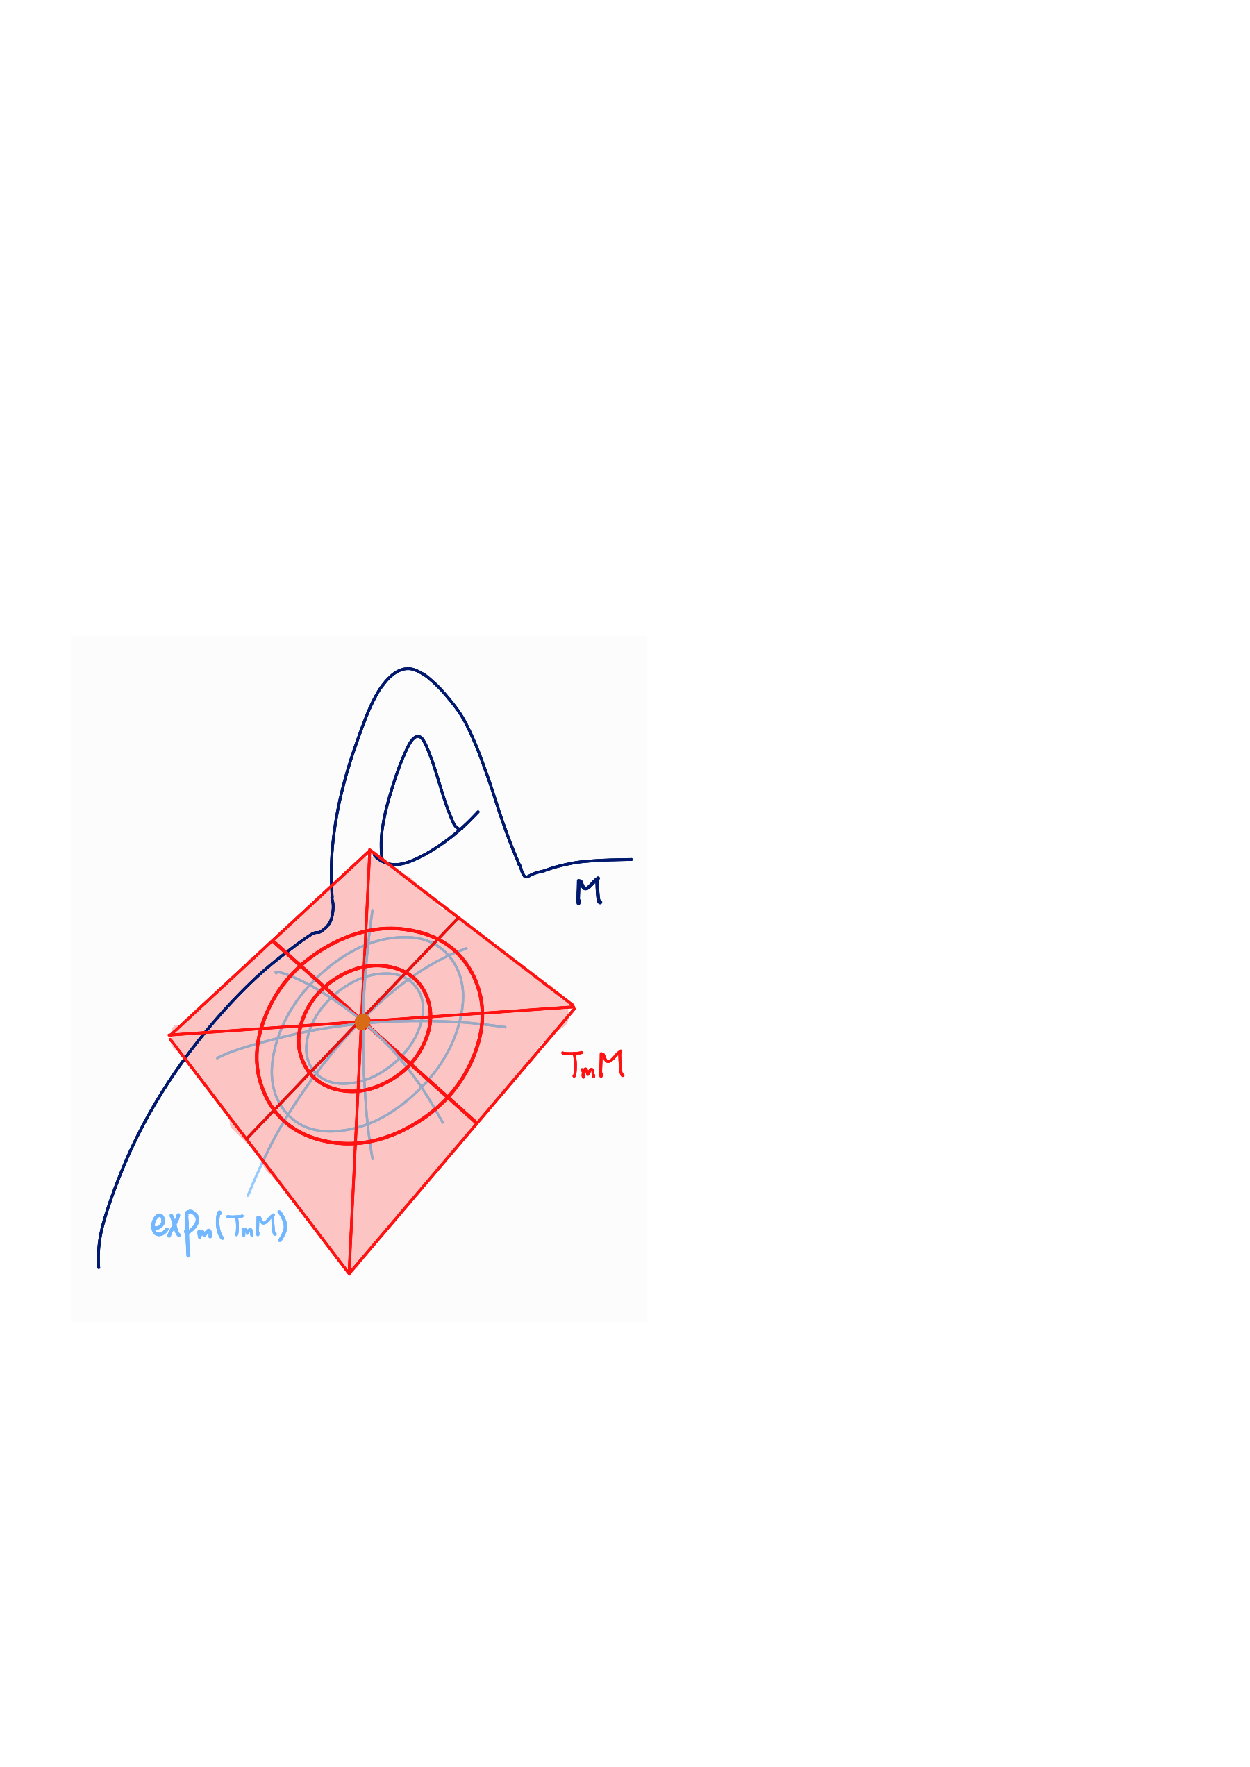
\includegraphics[scale=0.69]{expMap}
\end{center}

\begin{corT}
Let $M$ be a Riemannian manifold of dimension $d$. For all $p \in M$, there exists $\rho>0$ such that Riemannian polar coordinates maybe introduced on $B_\rho(p) \coloneqq \{ q \in M\mid d(p,q) \leq \rho \}$. For any such $\rho$ and $q \in \pd B_\rho(p)$, there exists a unique geodesic $c$ of shortest length $\mathcal{L}(c) = \rho$, connecting $p$ to $q$. In polar coordinates of $T_pM$, this geodesic $c$ is represented by $x(t) = (t,\phi_0)$, $0\leq t\leq \rho$, where $q$ represented by $(\rho, \phi_0)$ with $\phi_0 \in S^{d-1}$.
\end{corT}
\begin{proof}
The existence of $\rho$ is guaranteed by Theorem 6.2. We can take arbitrary curve of constant speed from $p$ to $q$, that is $c(t) = (r(t) ,\phi(t))$ for $0\leq t\leq T$, which does not have to entirely be contained in $B_\rho(p)$. Consider the following:
$$t_0 \coloneqq \inf\{ t\leq T \mid d(c(t),p) \geq \rho\}$$ 
then $t_0\leq T$ and $c|_{[0,t_0]}$ entirely lines in $B_\rho(p)$. We will show that $\mathcal{L}(c|_{[0,t_0]}) \geq \rho$ and $\mathcal{L}(c|_{[0,t_0]}) = \rho$ only for straight line in polar coordinates, where we define:
\begin{align*}
\mathcal{L}(c|_{[0,t_0]}) \coloneqq \int_0^{t_0}\left( g_{ij}(c(t)) \dot{c}^i\dot{c}^j\right)^{1/2} \, dt 
&\geq \int_0^{t_0}\left( g_{rr}(c(t)) \dot{r}\dot{r}\right)^{1/2}\, dt \\
&= \int_0^{t_0}|\dot{r}| \, dt \geq \int_0^{t_0}\dot{r}\, dt = r(t_0) = \rho
\end{align*}
where we have used the fact that $g_{r\phi}(c(t)) = 0$ and $g_{\phi\phi}(c(t))$ is positive definite. Straight lines in polar coordinates represent geodesics in $M$ by construction of the polar coordinates, hence that completes the proof. 
\end{proof}
\remark Under the assumptions of Corollary 6.2.1, the Euclidean ball $B_\rho(0)$ defined by:
$$ B_\rho(0)\coloneqq \{ y \in T_pM \mid |y|<\rho\} \subseteq T_pM$$ is mapped under $\exp_p$ diffeomorphically onto the Riemannian ball with the same radius $B_\rho(p) \subseteq M$.\\


\note If one has a compact manifold, such Riemannian polar coordinates can be introduced by Corollary 6.2.1 and there exists $\rho_0 >0$ such that any two points $p,q \in M$ with distance less than $\rho_0$ can be connected by a minimizing geodesic, that is a geodesic of shortest length. \\

\newpage
\section[Length Minimizing Geodesics]{\color{red} Length Minimizing Geodesics \color{black}}
\begin{thm}[Theorem 1.6.1 on \textit{Jost}]
Let $M $ be a compact Riemannian manifold, then any two points $a,b \in M$ can be connected by a length minimizing geodesic, and for all $p\in M$, $\exp_p$ can be defined on all of $T_pM$, any geodesic maybe extended indefinitely in any direction.
\end{thm}
\begin{proof}[Proof sketch]
The proof proceeds by utilizing a minimizing sequence $(\gamma_n)$ of curves in a homotopy class. Assuming each $\gamma_n$ is a piecewise geodesic joining the points $\{p_{n,1}, p_{n,2},\cdots, p_{n,m}\}$, we can construct a subsequence of $(\gamma_n)$ using the compactness of $M$ and the sequences $(p_{n,j})_{n\geq 1}$ of points. The limit of such subsequence of $(\gamma_n)$ is the desired minimizing geodesic. 
\end{proof}

In the most general setting, that is if a manifold is not compact, the result of Theorem 7.1 does not hold. We indeed require a manifold to be geodesically complete in order to obtain result similar to Theorem 7.1.

\begin{defn}
A Riemannian manifold is said to be geodesiccally complete provided that for all $p \in M$, $\exp_p$ can be defined on all of $T_pM$, that is, $M$ is geodesically complete provided that any geodesic $c(t)$ with $c(0) = p$ can be extended for all $t \in \R$.  
\end{defn}

\begin{corT}
On any compact Riemannian manifold $M$, any two points $p,q \in M$ can be connected by a geodesics of shortest length.
\end{corT}

\begin{corT}
Let $M$ be a compact Riemannian manifold. If a piecewise differentiable curve $\gamma:[a,b] \to M$ is parametrized proportional to the arc length, and has length less than or equal to the length of any other piecewise differentiable curves joining $\gamma(p)$ and $\gamma(b)$, then $\gamma$ is a geodesic, and is regular. 
\end{corT}

\begin{thm}[The Hopf-Rinow Theorem]
Let $M$ be a Riemannian manifold. The followings are equivalent:
\begin{enumerate}[topsep=3pt,itemsep=-1ex,partopsep=1ex,parsep=1ex]
\item $M$ is complete as a metric space. That is, $M$ is complete as a topological space with respect to the topology induced by the Riemannian metric. 
\item Closed and bounded subsets of $M$ are compact.
\item There exists $p \in M$ such that $\exp_p$ can be defined on all of $T_pM$.
\item $M$ is geodesically complete. 
\end{enumerate}
Each of the statements (1) to (4) implies (5) that every two points $p,q \in M$ can be joined by a length minimizing geodesic. 
\end{thm}
\begin{proof}
We will start by showing that (4) implies (5). Let $M$ be a geodesically complete manifold, given $p,q \in M$, let $r\coloneqq d(p,q)$. By Lemma 6.2.1, there exists $\rho$ such that Riemannian polar coordinates may be introduced on $B_\rho(p) \coloneqq \{ q' \in M | d(p,q') \leq \rho\}$. For any such $\rho$ and and $q' \in \pd B_{\rho}(p)$, there exists precisely one geodesic of shortest length $\rho$ connecting $p$ and $q'$. Let $p_0 \in \pd B_{\rho}(p)$ be a point where the continuous function $d(q,\cdot): M\to \R \ \ \ p'\mapsto d(p',q)$ attains it s minimum on the compact set $\pd B_{\rho}(p)$. Then for some $v \in T_pM$, we have $p_0 = \exp_p (\rho v)$. Consider the geodesic $c(t) = \exp_p (tv)$. We want to show that $c(r) = q$, in which case we know that $c|_{[0,r]}$ is the shortest geodesic from $p$ to $q$. \\

Here we define: 
$$I = \{t \in [0,r]\,|\, d(c(t),q) = r-t\}$$ 
We want to show that $I= [0,r]$. Here we view $I$ as a subspace of $[0,1]$. By construction, $I$ contains $0$, and $I$ is obviously closed by the continuity of $d$. To show that $I = [0,r]$, it suffices to show that $I$ is open in $[0,1]$. Let $t_0 \in I\setminus \{0\}$, and take $\rho_1>0$ to be the radius as in Lemma 6.2.1, WLOG, we can take $\rho_1<r-t_0$.  Let $p_1 \in \pd B_{\rho_1}(c(t_0))$ be a point such that the continuous function $d(q,\cdot)$ attains its minimum value on the compact set $\pd B_{\rho_1}(c(t_0))$. Then by triangle inequality, we can write the following:
\begin{align*}
d(p,q) \leq d(p,p_1) + d(p_1,q)
\end{align*}
For all curve $\gamma$ from $c(t_0)$ to $q$, there exists $\gamma(t) \in \pd B_{\rho_1}(c(t_0))$. Here we can write the following as $p_1$ is minimizing distance from $\pd B_{\rho_1}(c(t_0))$ to $q$:
\begin{align*}
\mathcal{L}(\gamma) \geq d(c(t_0), \gamma(t)) + d(\gamma(t),q) = \rho_1 + d(\gamma(t),q)\geq \rho_1 +d(p_1,q)
\end{align*}
That is, we have:
\begin{align*}
 d(q,c(t_0)) \geq \rho_1  + d(p_1,q)
\end{align*}
On the other hand, from triangle inequality, we have:
\begin{align*}
 d(q,c(t_0)) \leq \rho_1+ d(p_1,q)
\end{align*}
Hence we conclude that we have:
\begin{align*}
d(q,c(t_0)) = \rho_1 +d(p_1,q)
\end{align*}
rearranging we get:
\begin{align*}
d(p_1,q) = d(q,c(t_0)) - \rho_1 = r-t_0 - \rho_1
\end{align*}
Then combining we get:
\begin{align*}
d(p_1,p) \geq r- (r-t_0 -\rho_1) = t_0 + \rho_1
\end{align*}
Also, there exists a curve $\that{c}$ from $p$ to $p_1$ of length $t_0 + \rho_1$, with portion from $p$ to $c(t_0)$ along $c$, and portion being geodesic from $c(t_0)$ to $p_1$ of length $\rho_1$. By Theorem 7.1,, we know that $c'$ is a geodesic as it is the distance minimizer between points $p$ and $p_1$. The uniqueness of such geodesic with given initial data at $p$ implies that we have $c = \that{c}$. \\

Thus we have here $p_1  = c(t_0 +\rho_1)$, then we can write the following:
\begin{align*}
d(c(t_0+\rho_1), q) = d(p_1 q) = r-t_0 - \rho_1 = t-(t_0 +\rho_1)
\end{align*} 
that is, we see here $(t_0+\rho_1) \in I$, and hence $I$ is open, and it follows that $I = [0,r]$, and hence we conclude that $c(r) = q$. This completes the proof of (4) implies (5). \\

Now we will show the equivalency between (1), (2), (3), and (4). Note that (4) implies (3) is trivial. Now we will show that (3) implies (2). Let $K \subseteq M$ be a closed and bounded subset of $M$. Since $K$ is bounded, there $K \subseteq B_r(p)$ for some $r > 0$ and $p$ given by the statement of (3). Any point in $B_r(p)$ can be jointed with $p$ by a geodesic of length $\leq r$. That is $B_r(p)$ is the image of the compact ball in $T_pM$ of radius $r$ under the continuous map $\exp_p$. Then we know that $B_r(p)$ is compact, and since $K$ is a closed set contained in a compact set, we conclude that $K$ is compact. Next we will show that (2) implies (1). Let $(p_n)$ be a Cauchy sequence in the metric space $M$, then it is bounded.  By (2), the closure of the set of points of $(p_n)$ is compact. Therefore $(p_n)$ admits a convergent subsequence, and hence $(p_n)$ converges, which implies $M$ is complete as a metric space. Finally, we will show that (1) implies (4). Let $c$ be a geodesic in $M$ parametrized by arc length defined on a maximal interval $I$. By construction, $I$ is not empty, it is not hard to show that $I$ is both open and closed. The details is given in the proof of Theorem 1.7.1 on \textit{Jost}. These complete the proof. 
\end{proof}

\remark The converse of the Hopf-Rinow Theorem is not true. Consider the open half-sphere $B$. Any two points in $B$ can be joint by a unique minimal geodesic, but one can check that $B$ is not geodesically complete. \\

\begin{defn}
A diffeomorphism $h:M\to N$ between Riemannian manifolds $M$ and $N$ is called an isometry provided that $h$ preserves the Riemannian metric. That is, $h$ is an isometry provided that, for $p \in M$, $v,w \in T_pM$, we have the following holds:
\begin{align*}
\langle v,w\rangle_p = \langle dh(v), dh((w)\rangle_{h(p)}
\end{align*}
where $\langle \cdot, \cdot\rangle_p$ is the inner product, that defines the Riemannian metric on $M$, defined on $T_pM$, and $\langle \cdot,\cdot \rangle_{h(p)}$ is the inner product, that defines the Riemannian metric on $N$, defined on $T_{h(p)}N$. 
\end{defn}

\begin{defn}
A differentiable map $h:M \to N$ between Riemannian manifolds $M$ and $N$ is called a local isometry provided that for all $p \in M$, there exists a neighborhood $U$ of $p$ such that $h|_U:U \to h(U)$ is an isometry and $h(U)\subseteq N$ is open. 
\end{defn}

\begin{defn}
Let $M$ be a Riemannian manifold, let $p \in M$. \\
The injectivity radius of $p$ is defined by the following:
\begin{align*}
i(p) \coloneqq \sup\{\rho >0 \mid \exp_p\text{ is well-defined on }B_\rho(0) \in T_pM \text{ and is injective}\}
\end{align*}
The injectivity radius of $M$ is defined by the following:
\begin{align*}
i(M) \coloneqq \inf\{i(p) \mid p \in M\}
\end{align*}
\end{defn}

\example For $S^n$, we have $i(S^n) = \pi$. For torus $T^n$, we have $i(T^n) = \frac{1}{2}$. \\

\note The injectivity radius of a compact manifold is always greater than zero, which can be proved by simple continuity argument. However, the injectivity radius for a complete manifold might be zero. \\



\begin{thm}[Theorem 1.4.1 on \textit{Jost}]
Each differentiable manifold can be equipped with a complete Riemannian metric. 
\end{thm}

\example Consider the Poincare half-plane defined by:
\begin{align*}
P = \{(x,y) \in \R \mid y>0\}
\end{align*}
Here we equip $P$ with the induced Euclidean metric on $\R^2$. Clearly, $P$ is not complete because the line $y = 0$ is not included in $P$. However, $P$ becomes complete when equipped with the Poincare metric defined by the following:
\begin{align*}
ds^2 = \frac{dx^2 + dy^2}{y^2}
\end{align*}  
$P$ equipped with such metric is called the hyperbolic half-plane, denoted as $H^2$. \footnote{For more about the Poincare metric defined on the Poincare half-plane, check out \textit{Section 42 - Riemannian Metrics }in the text \textit{Class Note: Math 395/396 - Honors Analysis} transcribed by Jinyan Miao in Winter 2022.}\\




\example Take the quotient of the Poincare half-plane $P$ by the following transitions:
\begin{align*}
(x,y)\mapsto (x+n,y) \qquad\qquad n\in \Z
\end{align*}
One can check that we obtain a complete Riemanian manifold $M$ and the injectivity radius of $M$ is zero.\\

\remark Finding the lower bounds for the injectivity radius of a manifold involves curvature estimates. \\

\newpage
\chapter{Connections and Curvatures}
\setcounter{section}{7}
\section[Tensors and Vector Bundles]{\color{red}Tensors and Vector Bundles\color{black}}
\begin{defn}
A differentiable vector bundle of rank $n$ consists of a total space $E$, a base $M$ and a projection $\Pi:E \to M$, with $E,M$ being differentiable manifolds, $\Pi$ being differentiable, and each fiber $E_x\coloneqq \Pi^{-1}(x)$ for $x \in M$ carries structure of an $n$-dimensional real-valued vector space and that the local triviality condition holds, that is for all $x \in M$, there exists a neighborhood $U$ of $x$ and a diffeomorphism $\phi:\Pi^{-1}(U) \to U\times \R^n$ with the property that for all $y \in U$, $\phi|_y \coloneqq \phi|_{E_y} :E_y \to \{y\} \times \R^n$ is a vector space isomorphism. Here $(\phi,U)$ is called a bundle chart for the vector bundle $(E,M,\Pi)$. 
\end{defn} 

\remark Via Definition 8.0.0.0.1, a vector bundle can be viewed locally, but not necessarily globally, a product of its base and its fibers. A vector bundle $(E,M,\Pi)$ that is isomorphic to $M \times \R^n$ is said to be trivial. We may look at a vector bundle as a family of vector spaces all isomorphic to a fixed $\R^n$, parametrized locally trivially by a manifold $M$. 


\begin{defn} A vector field $X$ on a differentiable manifold $M$ is a correspondence that associates to each point $p \in M$ a vector $X(p) \in T_pM$. In terms of mappings, $X$ is a mapping of $M$ into the tangent bundle $TM$, that is $X:M \to TM$. The field $X$ is differentiable provided that $X:M \to TM$ is differentiable. 
\end{defn}

\note Let $M$ be a differentiable manifold of dimension $n$, consider a parametrization $x:U \to M$ with $U \subseteq \R$. For a vector field $X$ on $M$ and $x(t) = p \in M$, we can write:
\begin{align*}
X(p) = a_i(t) \left.\frac{\pd}{\pd x_i}\right|_{t}
\end{align*}
where each $a_i:U \to \R$ is a function on $U$ and $\{\pd/\pd x_i\mid 1\leq i \leq n\}$ is the basis associated to the parametrization $x$. Clearly, $X$ is differentiable if and only if all the functions $a_i$ are differentiable for any parametrization. In this sense, it is convenient to view a vector field $X$ as a mapping from the set $\mathcal{D}$ of differentiable real-valued functions on $M$ to the set $\mathcal{F}$ of real-valued functions on $M$, given in the following definition:
\begin{align*}
X:\mathcal{D} \to \mathcal{F} \qquad f\mapsto Xf
\end{align*}
where we write the following for $p \in M$:
\begin{align*}
Xf(p):M \to \qquad p\mapsto a_i(p) \left.\frac{\pd f}{\pd x_i}\right|_{p}
\end{align*}
Here $f$ denotes, intuitively, the expression of $f$ in the parametrization $x$. Indeed, one can check that the definition of $Xf$ does not depend on the choice of parametrization. \\


\begin{defn}
Let $M$ be a differentiable manifold. For vector fields $X,Y$ on $M$, the Lie bracket, or the bracket, of $X,Y$ is defined as the vector field:
\begin{align*}
[X,Y]\coloneqq X^j \frac{\pd Y^i}{\pd x^j} \frac{\pd}{\pd x^i} - Y^j \frac{\pd X^i}{\pd x^j}\frac{\pd}{\pd x^i} = XY - YX
\end{align*}
where $X = X^i \pd/\pd x^i$ and $Y = Y^i \pd/\pd x^i$, and the second equality can be verified easily.
\end{defn}
\remark The bracket $[X,Y]$ of vector fields can also be interpreted as a deviation of $Y$ along the trajectories of $X$, more details can be found in Section 5 in Chapter 0 on \textit{do Carmo}. 


\begin{prop}[Proposition 5.3 on \textit{do Carmo}]
Let $X,Y,Z$ be differentiable vector fields on a differentiable manifold $M$, let $a,b\in \R$, and let $f,g$ be differentiable real-valued functions defined on $M$, then we have:
\begin{enumerate}[topsep=3pt,itemsep=-1ex,partopsep=1ex,parsep=1ex]
\item $[X,Y ] = -[Y,X]$
\item $[aX + bY,Z] = a[X,Z] + b[Y,Z]$
\item $[[X,Y],Z] = [[Y,Z],X]+[[Z,X],Y]=0$
\item $[fX,gY] = fg[X,Y] +fX(g)Y - gY(f)X$
\end{enumerate} 
where (3) is called the Jacobi identity. 
\end{prop}


\begin{defn}
A $p$ times contravariant and $q$ times covariant tensor field on a differentiable manifold $M$ is a section of the following: 
$$\underbrace{TM\otimes TM \otimes  \cdots \otimes TM}_{p \text{ times}} \otimes \underbrace{T^*M \times T^*M \otimes \cdots \otimes T^*M}_{q \text{ times }}$$
\end{defn}


\begin{defn}
Let $V$ be a vector space of finite dimension $m$. The dual space of $V$ is denoted as $V^* = \{ \lambda: V\to \R\mid \lambda \text{ is linear}\}$. The vector space of $r$-times contravariant and $s$-times covariant tensors over $V$ is denoted as the following:
\begin{align*}
T_s^r(V) 
&=\left\{ A: \underbrace{V^*\times V^*\times \cdots \times V^*}_{r \text{ times}} \times \underbrace{V \times V \times \cdots \times V}_{s \text{ times}} \to \R\right\} \\
&= \underbrace{V\otimes V\otimes \cdots \otimes V}_{r \text{ times}} \times \underbrace{V^* \otimes V^* \otimes \cdots \otimes V^*}_{s \text{ times}} 
\end{align*}
\end{defn}

\begin{defn}
Let $(E,M,\Pi)$ be a vector bundle. A section of $E$ can be viewed as a differentiable map $s:M \to E$ that satisfies $\Pi\circ s = \mathbb{I}$, where $\mathbb{I}$ is the identity map defined on $M$. 
\end{defn}


\begin{defn}
Let $V$ be a finite dimensional vector space, we define the following for $s \in \N$: 
$$\Lambda^s(V^*)\coloneqq \{ A \in T_s^0 (V) \mid A\text{ is skew-symmetric}\}$$
Let $M$ be a manifold of dimension $m$, and let $(E, M, \Pi)$ be a $C^\infty$ vector bundle,
\begin{align*}
\Gamma(E) \coloneqq \{ s\in C^{\infty}(M,E) \mid \Pi \circ s = \mathbb{I}\}
\end{align*} 
\end{defn}

\begin{defn}
Let $M$ be a differentiable manifold, \\
we define the set of contravariant vector fields on $M$:
\begin{align*}
\Gamma(TM) = \left\{ \text{vector fields on $M$ with }TM = \bigcup_{p \in M}T_pM\right\}
\end{align*}
we define the set of covariant vector fields on $M$:
\begin{align*}
\Gamma(\Lambda_s M) = \left\{s\text{-forms on $M$ with }\Lambda_sM  = \Lambda^s\left( \bigcup_{p \in M}T_p^*M\right)\right\}
\end{align*}
and we define the following:
\begin{align*}
\Gamma (T_s^rM) = \{(r,s) - \text{tensor fields on }M\}
\end{align*}
Note that we also have:
\begin{align*}
T_s^rM = TM\otimes TM\otimes \cdots \otimes TM \otimes T^*M \otimes T^*\otimes \cdots \otimes T^*M
\end{align*}
\end{defn}

\example The Riemannian metric $g$ on a Riemannian manifold $M$ is a $(0,2)$-tensor field on $M$, that is, we have $g \in \Gamma(T_2^0(M))$, and for all $p \in M$, we have:
\begin{align*}
g(p):T_pM \times T_pM \to \R
\end{align*}


\begin{defn}
A pseudo-Riemannian metric on a differentiable manifold $M$ is a tensor field $g \in T_2^0(M)$ with the followings hold:
\begin{enumerate}[topsep=3pt,itemsep=-1ex,partopsep=1ex,parsep=1ex]
\item $g(p)(x,y) = g(p)(y,x)$ holds for all $x,y \in T_pM$ and all $p \in M$.
\item For all $p \in M$, $g(p)$ is non-degenerate bilinear form on $T_pM$, such that $g(p)(x,y) =0$ for all $x \in T_pM$ if and only if $y = 0$. 
\end{enumerate}
\end{defn}


\begin{defn}
A Lorentzian metric $g$ is a continuous assignment of non-degenerate quadratic forms $g(p)$ of index $1$ at $T_pM$ for all $p \in M$. The metric $g$ is non-degenerate at $p \in M$ provided that $g(p)(x,y) = 0$ for all $x \in T_pM$ if and only if $y = 0$. The non-degenerate quadratic form $g(p)$ is of index $1$ provided that the maximal dimension of a subspace of $T_pM$ on which the metric $g(p)$ is negative-definite is $1$. 
\end{defn}

\begin{defn}
A quadratic form $g(p)$ on $T_pM$ is said to be Lorentzian provided that there exists a vector $v\in T_pM$ such that $g(p)(v,v) < 0$ while $g(p)|_{\Sigma_v}$ is positive definite, where the set $\Sigma_v = \{x \mid g(p)(x,v) = 0\}$ is called the $g(p)$-orthogonal complement of $v$.  
\end{defn}

\newpage
\section[The Levi-Civita Connection]{\color{red}The Levi-Civita Connection\color{black}}
The motivation of defining a connection on a manifold arises as one wants to transport local geometric objects, such as tangent vectors, parallelly along the a curve on the manifold. However, such parallelism is not well-behaved under change of local coordinates on the manifold, and parallel transport always reflects the geometric properties intrinsic to the manifold. \\

In this text, for a differentiable manifold $M$, we denote elements in $\Gamma(TM)$ using capital letters $X, Y, Z$, etc, which are the vector fields on $M$. The notation $I$, when used as the domain of a geodesics, is considered to be a connected subset of $\R$. 

\begin{defn}
Let $M$ be a manifold. A vector field along a curve $c:I \to M$ is $X:I \to TM$ such that $X(t) \in T_{c(t)}M$ for all $t \in I$. We denote the set of smooth vector fields along a curve $c$ by $\chi_c(M)$. 
\end{defn}


\begin{defn}
Let $M$ be a differentiable manifold. A linear connection, or affine connection, denoted as $\nabla$ on $M$ is a bilinear map defined by the following:
\begin{align*}
\nabla: \Gamma(TM) \times \Gamma(TM) \to \Gamma(TM) \qquad (X,Y)\mapsto \nabla_XY
\end{align*}
where we have the followings hold for all $X,Y \in \Gamma(TM)$ and $f \in C^\infty(M,\R)$:
\begin{enumerate}[topsep=3pt,itemsep=-1ex,partopsep=1ex,parsep=1ex]
\item $\nabla_{fX}Y = f\nabla_X Y$
\item $\nabla_XfY = X(f)Y + f\nabla_XY$ 
\end{enumerate}
\end{defn}


\note Let $M$ be a differentiable manifold embedded in $\R^n$, and let $c:I \to M$ be a parametrized curve with $V:I \to M$ a vector field along $c$ tangent to $M$. The vector $dV/dt|_{t_0}$ with $t_0 \in I$ does not in general belong to the tangent plane $T_{c(t_0)}M$, hence we instead consider the orthogonal projection of $dV/dt|_{t_0}$ on $T_{c(t_0)}M$, which is denoted as $DV/dt|_{t_0}$ and is called the covariant derivative of $V$ at $c(t_0)$. 





\begin{prop}[Proposition 2.2 in Chapter 2 on \textit{do Carmo}]
Let $M$ be a differentiable manifold with an affine connection, and let $c:I \to M$ be a differentiable curve on $M$. There exists a unique correspondence which associates to a vector field $V$ along $c$ another vector field $DV/dt$ along $c$ such that the followings hold:
\begin{enumerate}[topsep=3pt,itemsep=-1ex,partopsep=1ex,parsep=1ex]
\item $(D/dt)(V+W) = DV/dt + DW/dt$ for any vector field $W$ along $c$.
\item $(D/dt)(fW) = (df/dt)V + f(DV/dt)$ for any vector field $W$ along $c$ and any scalar-valued differentiable function $f$ defined on $I$. 
\item If $V (t)= Y(c(t))$ for some vector field $Y$ on $M$, then $(DV/dt) = \nabla_{dc/dt}Y$. 
\end{enumerate}
The vector field $DV/dt$ along $c$ is called the covariant derivative of $V$.  
\end{prop}

\begin{defn}
A vector field $X$ along a curve $c:I \to M$ is said to be parallel provided that we have:
\begin{align*}
\frac{DX}{dt}  = 0
\end{align*}
The parallel transport from $c(t_0)$ to $c(t)$ along the curve $c$ on the manifold $M$ is the linear map $P_t : T_{c(t_0)}M \to T_{c(t)}M$ associating $v \in T_{c(t_0)}M$ to the vector $X_v(t)$ with $X_v$ being the parallel vector field along $c$ such that $X_c(t_0) = v$. 
\end{defn}


\begin{defn}
A connection $\nabla$ on a differentiable manifold $M$ is said to be compatible with the metric $g$ provided that for any smooth curve $c$ and any pair of parallel vector fields $P$, $P'$ along $c$, we have $g(P,P')$ being constant for all points on $c$.
\end{defn}

\begin{lem}[Proposition 3.2 in Chapter 2 on \textit{do Carmo}]
Let $M$ be a Riemannian manifold, a connection $\nabla$ on $M$ is compatible with a metric if and only if for any vector fields $V$ and $W$ along the differentiable curve $c:I \to M$, we have the following holds:
\begin{align*}
\frac{d}{dt}\langle V, W\rangle = \left\langle \frac{DV}{dt},\ W\right\rangle + \left\langle V, \ \frac{DW}{dt}\right\rangle
\end{align*}
\end{lem}

As from Lemma 9.0.2, we see that a connection $\nabla$ on a Riemannian manifold $M$ is compatible with the Riemannian metric $g$ if and only if we have:
\begin{align*}
X\langle Y, Z\rangle = \langle \nabla_X Y, Z \rangle + \langle Y, \nabla_X Z\rangle
\end{align*}
for any $X,Y,Z \in \Gamma(TM)$. Also from Lemma 9.0.2, we see that the parallel transport defines for all $t\in I$ an isometry from $T_{c(t_0)}M$ onto $T_{c(t)}M$. 

\begin{defn}
Let $\nabla$ be given as a linear connection on a differentiable manifold $M$, we define the torsion tensor of $\nabla$ as the following:
\begin{align*}
T:\Gamma(TM) \times \Gamma(TM) \to \Gamma(TM) \qquad (X,Y) \mapsto \nabla_XY - \nabla_YX - [X,Y]
\end{align*}
$\nabla$ is said to be torsion-free provided that $T(X,Y) = 0$ for all $X,Y \in \Gamma(TM)$. Let $g$ be a Riemannian metric on $M$ , then $\nabla $ is said to be Riemannian, or metric, provided that the following holds for all $X,Y,Z \in \Gamma(TM)$: \footnote{For a Riemannian metric $g$ on a differentiable manifold $M$, and for $X,Y \in \Gamma(TM)$, we abbreviate $g(p)(X(p),Y(p))$ as $g(X,Y)$ with $p \in M$. The Riemannian metric $g$ might also be denoted as $\langle \cdot, \cdot \rangle$.}
\begin{align}
Zg(X,Y)=g(\nabla_ZX,Y) + g(X,\nabla_Z Y)
\end{align}
\end{defn}

\remark The torsion gives an intrinsic characterization of how tangent spaces of a manifold twist about a curve on the manifold when they are parallel transported. On the other hand, the curvature, which will be introduced in the next section, describes how the tangent spaces roll along the curve. Torsion may be described concretely as a tensor  on the manifold as in Definition 9.0.2.0.1.

\begin{prop}
On each Riemannian manifold $M$, there exists a unique Riemannnian torsion-free connection $\nabla$ on $TM$, determined by the following:
\begin{align}
\langle \nabla_X Y,Z \rangle = \frac{1}{2}\left( X\langle Y,Z\rangle - Z\langle X,Y\rangle + Y \langle Z, X\rangle - \langle X,[Y,Z]\rangle + \langle Z, [X,Y]\rangle + \langle Y, [Z,X]\rangle\right)
\end{align}
\end{prop}
\begin{proof}
Each Riemannian torsion-free connection must satisfies (3.1), from which  (3.2) can be derived and hence implying the uniqueness of such $\nabla$. The existence of $\nabla$ is to verify that the unique map $\nabla:\Gamma(TM) \times \Gamma(TM) \to \Gamma(TM)$ given by (3.2) satisfies all desired properties of being a linear connection.
\end{proof}

\begin{defn}
For a Riemannian manifold $M$, the linear connection on $TM$ defined by (3.2) is called the Levi-Civita connection on $TM$. 
\end{defn}


\newpage
\section[The Riemannian Curvature Tensor]{\color{red} The Riemannian Curvature Tensor\color{black}}
\begin{defn}
Let $M$ be a Riemannian manifold, and let the Levi-Civita connection be given on $TM$. The Riemannian curvature tensor is a map defined by the following:
\begin{align*}
R:\Gamma(TM) \times \Gamma(TM) \times \Gamma(TM) \to \Gamma(TM) \ \ \ (X,Y,Z) \mapsto \nabla_X\nabla_Y Z - \nabla_Y\nabla_X Z - \nabla_{[X,Y]}Z
\end{align*}
Here we denote $R(X,Y)Z = \nabla_X\nabla_Y Z - \nabla_Y\nabla_X Z - \nabla_{[X,Y]}Z$. 
\end{defn}

\remark One way to interpret the Riemannian curvature tensor is that it assigns a tensor to each point of the Riemannian manifold. The tensor field measures the failure of the second covariant derivatives to commute. A Riemannian manifold has zero curvature if and only if it is flat, that is locally isometric to the Euclidean space.\\


To develop the geometric intuition for the Riemannian curvature tensor, consider the coordinate vector fields $\pd /\pd x^i$ from which we obtain the followings:
\begin{align*}
\left[\frac{\pd}{\pd x^i}, \frac{\pd}{\pd x^k} \right] = 0
\qquad \Rightarrow\qquad 
R\left( \frac{\pd}{\pd x^i}, \frac{\pd}{\pd x^j}\right) \frac{\pd}{\pd x^l} = R^k_{lij}\frac{\pd}{\pd x^k}
\end{align*}
where we have: \footnote{The detailed derivation is given on \textit{Jost} Section 4.1 in Chapter 4.}
\begin{align*}
R_{lij}^k \coloneqq \Gamma_{jl,i}^k - \Gamma_{il,j}^k + \Gamma_{im}^k\Gamma_{jl}^m - \Gamma_{jm}^k\Gamma_{il}^m
\end{align*}
One can define:
\begin{align*}
R_{klij}  \coloneqq g_{km}R^{m}_{lij}
\end{align*}
and we obtain:
\begin{align}
R_{klij} = \left\langle R \left( \frac{\pd}{\pd x^i}, \frac{\pd}{\pd x^j}\right) \frac{\pd}{\pd x^l}
, \frac{\pd}{\pd x^k}\right\rangle
\end{align}

\begin{defn}
Given the Riemannian curvature tensor $R:\Gamma(TM) \times \Gamma(TM) \times \Gamma(TM) \to \Gamma(TM)$ on a Riemannian manifold $M$, here we define the sectional curvature of the plane spanned by the tangent vectors $X,Y \in T_xM$, where we denote $X = \xi^i(\pd/\pd x^i) $ and $Y = \eta^i (\pd /\pd x^i)$:
\begin{align*}
K(X\wedge Y) \coloneqq \frac{\langle R(X,Y)Y, X\rangle }{|X\wedge Y|^2}
\end{align*}
where we have:
\begin{align*}
|X \wedge Y |^2 = \langle X,X\rangle \langle Y,Y\rangle  - \langle X,Y\rangle^2
\end{align*}
\end{defn}
From definition 10.0.0.0.2, it is not hard to obtain:
\begin{align*}
K(X,\wedge Y) = \frac{R_{ijkl}\xi^i \eta^j \xi^k \eta^l}{g_{ik}g_{jl}(\xi^i\xi^k \eta^j\eta^l - \xi^i\xi^j \eta^k \eta^l)} = \frac{R_{ijkl}\xi^i \eta^j \xi^k \eta^l}{(g_{ik}g_{jl} - g_{ij}g_{kl})\xi^i \eta^j \xi^k\eta^l}
\end{align*}


\begin{defn}
Given the Riemannian curvature tensor $R:\Gamma(TM) \times \Gamma(TM) \times \Gamma(TM) \to \Gamma(TM)$, here we define the Ricci curvature tensor:
\begin{align*}
R_{ab} = g^{cd}R_{cadb}
\end{align*}
the Ricci curvature in the direction of vector field $X$ on the Riemannian manifold $M$ is given as the following:
\begin{align*}
\text{Ric}(X,X) \coloneqq g^{il}\left\langle R\left(X, \frac{\pd}{\pd x^j}\right)\frac{\pd}{\pd x^l},\ X\right\rangle
\end{align*}
and the scalar curvature is given as the following:
\begin{align*}
R = g^{ab}R_{ab}
\end{align*}
\end{defn}

\begin{lem}[First Bianchi Identity, Lemma 4.3.1 on \textit{Jost}]
From definition given in (3.3), we have:
\begin{align*}
R_{klij} + R_{kijl} + R_{kjli} = 0
\end{align*}
Equivalently, for vector fields $X,Y,Z,W$ on $M$, and the Riemannian curvature tensor $R$ on the Riemannian manifold $M$, we can write:
\begin{align*}
R(X,Y)Z + R(Y,Z)X + R(Z,X)Y = 0
\end{align*}
\end{lem}
\begin{lem}[Second Bianchi Identity, Lemma 4.3.2 on \textit{Jost}]
From definition given in (3.3), we have:
\begin{align}
\frac{\pd}{\pd x^h}R_{klij} + \frac{\pd}{\pd x^k}R_{lhij} + \frac{\pd}{\pd x^l} R_{hkij} = 0
\end{align}
\end{lem}

\hfill\break
\hfill\break
We claim that the following gives an alternative definition for the geodesic:

\begin{defn}
Let $\nabla$ defined on $TM$ be a linear connection of a differentiable manifold $M$. A curve $c: I  \to M$ is called a geodesic with respect to $\nabla$ provided that we have the following holds:
\begin{align*}
\nabla_{\dot{c}}\dot{c} = 0
\end{align*}
\end{defn}
Given the settings in Definition 10.0.2.0.1, in local coordinates, we can write:
\begin{align*}
\dot{c} = \dot{c}^i \frac{\pd}{\pd x^i}
\end{align*}
in which case we can write the following:
\begin{align*}
\nabla_{\dot{c}}\dot{c} = \dot{c}^i \nabla_{\pd/\pd x^i}\dot{c}^j \frac{\pd}{\pd x^j} = \dot{c}^i \dot{ c}^j \Gamma_{ij}^k \frac{\pd}{\pd x^k} + \ddot{c}^k \frac{\pd}{\pd x^k} = \left(\ddot{c}^k + \Gamma_{ij}^k \dot{c}^i \dot{c}^j \right)\frac{\pd}{\pd x^k} =0
\end{align*}
recovering (2.3) which gives the former definition of geodesic. \\



\newpage
\chapter{Flows on Manifolds}
\setcounter{section}{10}
\section[Flows of Vector Fields]{\color{red}Flows of Vector Fields\color{black}}
\begin{defn}
Let $M$ be a differentiable manifold, and let $X$ be a smooth vector field on $M$, which is a smooth section of the tangent bundle $TM$. Then $X$ defines a system of first order differentiable equations as the following:
\begin{align*}
\dot{c} = X(c)
\end{align*}
The curve $c:I \to M$, with $I \subseteq \R$, describes the flow of the vector field $X$.  
\end{defn}

\note Let $M$ be a differentiable manifold. For all $p \in M$, we are interested in finding an open interval $I_p$ around $0 \in \R$ and a solution of the following ODE for some curve $c:I \to M$, and a vectoe field $X$ on $M$:
\begin{align*}
\left.\frac{dc}{dt}\right|_{t'} = X(c(t')) \qquad \text{with }t' \in I\qquad\qquad\qquad c(0) = p
\end{align*}
In local coordinates, this is a system of ODE. In such coordinates, we denote $c(t)$ as:
\begin{align*}
c(t) = (c^1(t), c^2(t), \cdots, c^d(t)) \qquad\text{with }d= \dim(M)
\end{align*}
Let $X$ be denoted as $X^i (\pd/\pd x^i)$, we have the following system defined by $1\leq i \leq d$:
\begin{align}
\left.\frac{dc^i}{dt}\right|_{t'} = X^i(c(t')) \qquad\text{with }t'\in I \qquad\qquad\qquad c(0) = p
\end{align}
The solution to (4.1) exists by Cauchy-Lipchitz Theorem for given initial data, and the solution is unique and smoothly dependent on the initial data. \\

\begin{prop}
Let $M$ be a differentiable manifold, and let $X$ be a vector field on $M$. For all $p \in M$, there exists an open interval $I_p \subseteq \R$ such that $0 \in I_p$ and a smooth curve $c_p:I_p \to M$ that solves the following system:
\begin{align}
\left.\frac{dc_p}{dt}\right|_{t'} = X(c_p(t'))\qquad \text{with }t' \in I \qquad\qquad\qquad c_p(0) = p
\end{align}
Furthermore, the solution to (4.2) depends smoothly on initial data.
\end{prop}

\begin{prop}
Let $M$ be a differentiable manifold, and let $X$ be a vector field on $M$. For all $p \in M$, there exists an open neighborhood $U$ of $p$ and an open interval $I$ with $0 \in I$ such that, for all $q \in U$, the curve $c_q$ defined by $\dot{c}_q(t) = X(c_q(t))$, $c_q(0) = q$, is well defined on $I$. The map $f:I\times U \to M \ \ \ (t,q) \mapsto c_q(t)$ is smooth. 
\end{prop}


\begin{defn}
Let $M$ be a differentiable manifold, and let $X$ be a vector field on $M$. The map $f:I \times  U \to M \ \ \ (t,q) \mapsto c_q(t)$ proposed in Proposition 11.0.2 is called the local flow of the vector field $X$. The curve $c_q$ is called the integral curve of $X$ through $q$. Furthermore,  we can define a local diffeomorphism $\varphi_t(q) \coloneqq c_q(t)$.
\end{defn}

\note In the settings of Definition 11.0.2.0.1, one can show that we have $(\varphi_{t}\circ \varphi_s) (q) = \varphi_{t+s}(q)$ for $s,t\in I$ that satisfies $t+s\in I$. If $\varphi_t$ is defined on $U \subseteq M$, then $\varphi_t$ maps $U$ diffeomorphically onto its image. \\

\begin{defn}
Let $M$ be a differentiable manifold, and let $X$ be a vector field on $M$. The family $\{\varphi_t \mid t \in I\}$ of diffeomorphisms from subsets of $M$ to subsets of $M$ defined by Definition 11.0.2.0.1 is called a local $1$-parameter group of diffeomorphisms associated to the vector field $X$.
\end{defn} 

\remark In general, local $1$-parameter group need not be extendible to a group because the maximal interval of definition $I$ need not be all of $\R$. \\

\example Consider the case where $M = \R$ and vector field $X(\tau) = \tau^2 (d/d\tau)$. In such case, (4.1) reads the following:
\begin{align*}
\dot{c}(t) = c^2(t)
\end{align*}
Given initial values, one can show that $c$ is not defined on all of $\R$. 

\begin{thm}
Let $X$ be a vector field on a differentiable manifold $M$ with compact support. Then the flow of $X$ is defined for all $q \in M$ on all of $\R$. The local $1$-parameter group defines a group of diffeomorphisms. 
\end{thm}

\begin{corT}
On a compact differentiable manifold $M$, any vector field on $M$ generates a $1$-parameter group of diffeomorphisms. 
\end{corT}


\newpage
\section[Cogeodesic Flow]{\color{red} Cogeodesic Flow\color{black}}
The Euler-Lagrange Equations is a system of second order ODE with $d$ equations in $d$-dimension. That can be transformed into a system of first order ODE with $2d$ equations. \\

Let $M$ be a differentiable manifold of dimension $d$. The Euler-Lagrange Equation, as proposed by (2.3), is given by the following:
\begin{align}
\ddot{x}^i(t) + \Gamma_{jk}^i (t) \dot{x}^j(t) \dot{ x}^k(t) = 0 \qquad\qquad\qquad \forall i\in\{1,2,\cdots,d\}
\end{align}
We will transform (4.3) into first doer system on the cotangent bundle $T^*M$. First we locally trivialize $T^*M$ by a chart $T^*M|_U \cong U \times \R^d$ with coordinate denoted as $(x^1,x^2,\cdots, x^d, p_1,p_2,\cdots,p_d)$. Now we set:
\begin{align*}
\mathcal{H}(x,p) = \frac{1}{2}g^{ij}(x) p_ip_j
\end{align*}
Here $\mathcal{H}$ is called the Hamiltonian of the system. Note that we have $g^{ik}g_{kj} = \delta_{ij}$.\\

\begin{thm}
For a differentiable manifold $M$ of dimension $d$. (4.3) is equivalent to the following system on $T^*M$: \footnote{The notation $\cdot_{,i}$ is a shorthand for $\pd/\pd x^i$}
\begin{align}
\dot{x}^i = \frac{\pd \mathcal{H}}{\pd p_i} = g^{ij}(x) p_j \qquad\qquad\qquad
\dot{p}_i = -\frac{\pd \mathcal{H}}{\pd x^i} = -\frac{1}{2}g^{ik}_{\ ,i}(x) p_j p_k
\end{align}
\end{thm}

\begin{defn}
For a differentiable manifold of dimension $d$. The flow determined by (4.4) is called the cogeodesic flow. The geodesic flow on $TM$ is obtained from the cogeodesic flow by the first equation in (4.4).
\end{defn}

\remark The cogeodesic flow is a Hamiltonian flow for the Hamiltonian $\mathcal{H}$. \\

From (2.10), along the integral curves, we can write the following:
\begin{align*}
\frac{\pd \mathcal{H}}{\pd t} = \mathcal{H}_{x^i}\dot{x}^i + \mathcal{H}_{p_i}\dot{p}^i = -\dot{p}_i \dot{x}^i + \dot{x}^i\dot{p}_i =0
\end{align*}
We observe that the cogeodesic flow maps the set $E_\lambda$ defined by the following onto itself for all $\lambda \geq 0$:
\begin{align*}
E_\lambda \coloneqq \{(x,p) \in T^*M \mid \mathcal{H}(x, p) = \lambda \}
\end{align*}
If $M$ is compact, then all $E_\lambda$ are also compact, the geodesic flow defined on all of $E_\lambda$ for all $\lambda$. Also, we have:
\begin{align*}
M = \bigcup_{\lambda \geq 0}PE_\lambda
\end{align*}
where $P$ is the projection. \\

\newpage


\begin{thm}
Let $M$ be a Riemannian manifold, let $D$ denote the cononical Levi-Civita connection, and let $c$ be a curve in $M$. There exists a unique operator $D/dt$ defined on the vector space of vector fields along $c$ satisfying the followings:
\begin{enumerate}
\item For all real functions defined on $I$, we have:
$$\frac{D}{dt} (fy)(t) =f'(t)y(t) + f(t) \frac{D}{dt}y(t)$$
\item For $v,w$, we have:
\begin{align*}
\frac{D}{dt}(v+w) = \frac{Dv}{dt} + \frac{Dw}{dt}
\end{align*}
\item If there exists a neighborhood of $t_0 \in I$ such that $y$ is the restriction to $c$ of a vector field $X$ defined on a neighborhood of $c(t_0)$ in $M$, then we have:
\begin{align*}
\frac{D}{dt}y(t_0) = \left( D_{c'(t_0)}X\right))_{c(t_0)}
\end{align*}
\end{enumerate}
\end{thm}
\begin{proof}
Let $X = X^i \pd_i$ and $V = V^k\pd_k$. $D$ is the Levi-Civita connection. Then we can write:
\begin{align*}
D_vX = D_v(X^i \pd_i) = v(X^i)\pd_i + X^i D_v\pd_i = v(X^i)\pd_i + V^kX^i\Gamma_{ki}^j \pd_j
\end{align*}
The covariant derivative along $c$ is defined by the following:
\begin{align*}
\frac{D}{dt}(y^i(t) \pd_i) = \frac{dy^i}{dt}\pd_i +\dot{c}y^i \Gamma_{ji}^k(c(t))\pd_x
\end{align*}
where $\dot{c} = \dot{c}^k \pd_k$. It follows from here that we have (1) and (2) hold. Now we will check (3). Let $X$ be a smooth vector field in $M$. Then the induced vector field along $c$ is given by the following:
\begin{align*}
y(t) = X_{c(t)}
\end{align*}
Note that we can write:
\begin{align*}
y(t) = y^i(t) \pd_i \qquad\qquad X_x = X^i(x) \pd_i \qquad\qquad y^i(t) = X^i(c(t))
\end{align*}
Then we have:
\begin{align*}
D_{\dot{c}}X &= D_{\dot{c}}(X^i \pd_i) \\
&= \dot{c}(X^i) \pd_i+X^i D_{\dot{c}}\pd_i\\
&=  \dot{c}(X^i) \pd_i + X^i \dot{c}^k D_{\pd_k}\pd_i \\
&= \pd_t (X^i \circ c) \pd_i + \dot{c}^k X^i \Gamma_{ki}^l \pd_l \\
&= \pd_t(X^i \circ ) \pd_i + \dot{c}^k y^k \Gamma_{ki}^l \pd_l \\
&= \frac{D}{dt}y
\end{align*}
\end{proof}

\remark We do not define $Dy/dt$ via (3) in the statement of Theorem 9.2 because a vector field $y$ along a curve $c$ may not always be extended to a neighborhood of $c$ in $M$. In local coordinates, we can write:
\begin{align*}
y(t) = y^i(t) \left.\frac{\pd}{\pd x^i}\right|_{c(t)}
\end{align*}
A vector field along a curve $c$ is always a linear combination of vector fields along $c$ that can be extended. 


\newpage
For a differentiable manifold $M$, elements in $T^*M$ are called the cotangent vectors, that is the linear functionals $\alpha\in T^*_xM$ such that $\alpha:T_xM \to F$. The sections of $T^*M$ are $1$-forms, that is $\alpha:TM\to \R$ with $\alpha|_x = \alpha|_{T_x{M}}\to \R$. Elements of $TM$ (ADD).\\


A Riemannian metric induces bundle metrics on all tensor bundles over the manifold. The metric of the cotangent bundle $T^*M$ is then given by the following:
\begin{align*}
\langle \omega, \eta\rangle = g^{ij}\omega_i \eta_i
\end{align*}
where $\omega = \omega_i dx^i$ and $\eta = \eta_i dx^i$.\\ 

The identification between $TM$ and $T^*M$ through the Riemannian metric:
\begin{align*}
V = V^i \frac{\pd}{\pd x^i}\in TM \qquad \text{ corresponds to }\qquad \omega = \omega_j dx^j \in T^*M
\end{align*}
with the following:
\begin{align*}
\omega_j = g_{ij}V^i \qquad\text{ or }\qquad V^i = g^{ij} \omega_j
\end{align*}
that we have:
\begin{align*}
g(x,y) &= g_{ij}X^i Y^j\qquad\qquad\forall X,Y \in TM\\
g(\omega, \eta) &= g^{ij}\omega_i \eta_j \qquad\qquad \forall \omega,\eta \in T^*M
\end{align*}



\newpage
Let $M,N$ be differentiable manifolds, let $f:M \to N$ be a differentiable map, let $(E,\Pi, N)$ be a vector bundle over $N$. We want to pull back the bundle $(E,\Pi, N)$ via $f$, that is, we want to construct a bundle $f^*E$ for which the fiber over $x \in M$ is $E_{f(x)}$. 

\begin{defn}
The pulled back bundle $f^*E$ is the bundle over $M$ with the bundle charts $\left( \varphi \circ f,\ f^{-1}(U)\right)$ with $(\varphi, U)$  being bundle charts of $E$. 
\end{defn}

\begin{defn}
Consider two vector bundles over $M$, $(E_1,\Pi_1,M)$ and $(E_2, \Pi_2,M)$, and consider a differentiable map $f:E_1 \to E_2$ that is fiber preserving, that is $\Pi_2 \circ f = \Pi_1$. $f$ is called a bundle homomorphism provided that the fiber maps $f_x:E_{1,x} \to E_{2,x}$ are linear, that is, $f$ is a bundle homomorphism provided that $f_x$ are vector space homomorphisms.
\end{defn}

\begin{defn}
Consider a vector bundle $(E,\Pi,M)$ of rank $n$, let $E' \subseteq E$. Assume that for all $x \in M$, there exits bundle chart $(\phi,U)$ such that $x \in U$ and $\phi(\Pi^{-1}(U) \cap E') = U \times \R^m \subseteq U\times \R^n$ where $m \leq n$. The so constructed vector bundle $(E', \Pi|_{E'}, M)$ is called the subbundle of $E$ of rank $m$. 
\end{defn}

Identification between $TM$ and $T^*M$ through Riemannian metric.\\

Let $V = V^i (\pd/ \pd x^i) \in TM$ corresponds to $w = w_j dx^j \in T^*M$, with $w_j$ be defined by the contraction with metric:
\begin{align*}
w_j = g_{ij}V^i \coloneqq V_j \qquad\qquad\qquad V^i = g^{ij}w_j
\end{align*}
Here we also have:
\begin{align*}
g(X,Y) = g_{ij}X^iY^i\qquad\qquad \text{for }X,Y \in TM
\end{align*}
\begin{align*}
g(\omega, \eta) = g^{ij}\omega_i \eta_j \qquad\qquad \omega, \eta \in T^*M
\end{align*}
(($X,Y$ are viewed as vector fields??))\\

A Riemannian metric induce bundle metrics on all tensor bundles over $M$. Metric of $T^*M$ is given by:
\begin{align*}
\langle \omega, \eta\rangle = g(\omega, \eta) = g^{ij}w_i\eta_j \qquad \text{ for }\omega = \omega_i\, dx^i, \ \eta = \eta_i\, dx^i
\end{align*}

Thus, for $V \in T_xM$, there corresponds a $1$-form $\omega \in T^*_xM$ via the metric:
\begin{align*}
\omega(Y) \coloneqq g(V,Y)\qquad \forall Y \in T_xM
\end{align*}
in which case we can identify $||\omega|| = ||V||$.\\


Let $(e_i)_{i \in \{1,2,\cdots, d\}}$ be a basis of $T_xM$, and let $(\omega^j)_{j \in \{1,2,\cdots, d\}}$ be a basis of the dual basis of $T^*_xM$. That is, we write:
\begin{align*}
\omega^j(e_i) = \delta_{ij}
\end{align*}
Let $V = V^i e_i \in T_xM$, and let $\eta = \eta_j\omega^j \in T_x^*M$. Then we can write:
\begin{align*}
\eta(V) = \eta_iV^i
\end{align*}
Consider bases $(e_i)$ and $(\omega^j)$ in local coordinates:
\begin{align*}
e_i = \frac{\pd}{\pd x^i} \qquad\qquad\qquad \omega^j = dx^j
\end{align*}
Let $f$ be a coordinate change, then $V$ transforms to the following:
\begin{align*}
f_*(V)\coloneqq V^i\, \frac{\pd f^\alpha}{\pd x^i}\, \frac{\pd}{\pd f^\alpha}
\end{align*}
and $\eta$ transforms to the following:
\begin{align*}
f^*(\eta) \coloneqq \eta_j\, \frac{\pd x^j}{\pd f^\beta}\, df^{\beta}
\end{align*}
Therefore, we have:
\begin{align*}
f^*(\eta) (f_*(V)) = \eta_j\, \frac{\pd x^j}{\pd f^\alpha}\,V^i\, \frac{\pd f^\alpha}{\pd x^i} = \eta_i V^i  = \eta(V)
\end{align*}
Thus the tangent vector transforms with functional matrix of coordiante change, and the cotangent vector transforms with the transposed inverse of the functional matrix of the coordinate change. \\

\example We compute the coordinate change for the followings:
\begin{align*}
\omega = \omega_i\, dx^i \qquad\qquad\qquad \eta = \eta_i\,dx^i
\end{align*}
Here we can write:
\begin{align*}
\langle \omega, \eta\rangle = g^{ij}\omega_i \eta_j
\end{align*}
Consider a coordinate change $y \mapsto x(y)$. Then we can write:
\begin{align*}
\omega_i dx^i = \omega_i \,\frac{\pd x^i}{\pd y^\alpha}\, dy^\alpha = \that{\omega}_\alpha dy^\alpha
\end{align*}
Note that $g^{ij}$ is transformed as:
\begin{align*}
h^{\alpha\beta} = g^{ij}\, \frac{\pd y^{\alpha}}{\pd x^i}\, \frac{\pd y^{\beta}}{\pd x^j}
\end{align*}
and hence we have:
\begin{align*}
h^{\alpha\beta}\that{\omega}_\alpha \that{\eta}_\beta = g^{ij}\omega_i \omega_j
\end{align*}
On the other hand, we have:
\begin{align*}
|| \omega(x) || = \sup\{ \omega(x) V \mid V \in T_xM, \ ||V|| = 1\}
\end{align*}


\newpage
The Lie brackets are defined for vector fields $X,Y$:
\begin{align*}
[X,Y] = XY - YX
\end{align*}
Note that the Lie bracket is a vector field.
\begin{defn}
Consider $X$ as a vector field on a Riemannian manifold $M$, with local $1$-parameter group $(\psi_t)_{t \in I}$ of local diffeomorphisms. Let $S$ be a tensor field on mM , the Lie derivative of $S$ in the direction of $X$ is defined as the following:
\begin{align*}
L_XS\coloneqq \frac{d}{dt}\left( \psi_t^* S\right) |_{t=0} 
\end{align*}
\end{defn}

\newpage
Let $\Psi:M \to N$ be a diffeomorphism where $M,N$ are differentiable manifolds. Let $X$ be a vector field on $M$, we can define a vector field $Y = \Psi_*X$ on $N$ by the following:
\begin{align*}
Y(p) = d\Psi (X(\Psi^{-1}(p))
\end{align*}

\begin{lem}
For every differentiable function $f:N \to \R$, we have the following holds:
\begin{align*}
(\Psi_*X)(f)(p) = X(f\circ \Psi)(\Psi^{-1}(p))
\end{align*}
Let $X$ be a vector field on $M$, and consider $\Psi:M \to N$ be a diffeomorphism, if local $1$-parameter group generated by $X$ is $(\psi_t)$, then the local group generated by $\Psi_*X$ is given by:
\begin{align*}
\Psi \circ \psi_t \circ \Psi^{-1}
\end{align*}
\end{lem}



Let $X = X^i \frac{\pd}{\pd x^i}$ be a vector field. We get a curve $X_t$ in $T_xM$ for $t \in I$, and we want to differentiate such curve. We consider the following:
\begin{align*}
\left( \psi_{-t}\right)_* \frac{\pd}{\pd x^i}\left( \psi_t(x) \right) = \frac{\pd \psi_{-t}^k}{\pd x^i} \frac{\pd}{\pd x^k} 
\end{align*}
For $\varphi:M \to N$, we have:
\begin{align*}
\varphi_*\frac{\pd}{\pd x^i} = \frac{\pd \varphi^k}{\pd x^i}\frac{\pd}{\pd \varphi^k}
\end{align*}
For $M = N$, if $x$ and $\varphi(x) $ lie in the same neighborhood, we obtain:
\begin{align*}
\frac{\pd}{\pd \varphi^k} = \frac{\pd}{\pd x^k}
\end{align*}
Let $\omega = \omega_i dx^i$ be a $1$-form, then we can write:
\begin{align*}
\left( \psi^*_t\right) (\omega)(x) = \omega_i \left( \psi_t(x) \right) \frac{\pd \psi_t^i}{\pd x^k}\, dx^k
\end{align*}
which defines a curve in $T_x^*M$.\\

For $\varphi:M \to N$ and $1$-form $\omega = \omega_i dx^i$ on $N$, we have:
\begin{align*}
\varphi^*\omega \coloneqq \omega_i(\varphi(x) ) \frac{\pd z^i}{\pd x^k}dx^k
\end{align*}
Let $\varphi:M \to N$ be a diffeomorphism, and let $Y$ be a vector field on $N$, we can set:
\begin{align*}
\varphi^*Y \coloneqq (\varphi^{-1})_* Y
\end{align*}
In particular, for $X$ being a vector field, and local 1-parameter group $(\psi_{t})_{t \in I}$, we have:
\begin{align*}
\left( \psi_t^*X\right) = \left(\psi_{-t}\right)_* X
\end{align*}

Let $x \in M$, and let $X \in T_xM$, $df_xL T_xM \to T_{f(x)}M$. Then $df_xX$ or $(f_*)_xX$ is called the pushforward of $X$ by $f$. \\

Let $\omega \in T^*M$, being a $1$-form on $N$, then $(f^*\omega)_xX = \omega(f(x)) \left( df_x(X)\right)$ is called the pullback of $\omega$ by $f$, and $f^*\omega$ is a $1$-form defined on $M$.\\


\newpage
Recall that the Riemannian curvature tensor is defined by the following:
\begin{align*}
R(X,Y)Z = \nabla_X\nabla_Y Z - \nabla_Y\nabla_XZ - \nabla_{[X,Y]}Z
\end{align*}
\begin{defn}
The sectional curvature of the plane spanned by linearly independent tangent vectors $X = X^i (\pd/\pd x^i), \ Y = Y^i (\pd/\pd x^i)\in T_xM$ of the Riemannian manifold $M$ is given by:
\begin{align*}
K(X\wedge Y)\coloneqq \frac{g(R(X,Y)Y,X)}{|X\wedge Y|^2}
\end{align*}
where we have:
\begin{align*}
|X\wedge Y|^2 = g(X,X) g(Y,Y) - g(X,Y)^2
\end{align*}
\end{defn}


\remark A sectional curvature determines the whole Riemannian curvature tensor. That is, $g(R(X,Y)Z,W)$ can be expressed entirely by $K$.\\

For $2$-dimensional manifold $M$. We can write:
\begin{align*}
R_{ijkl} = K\left( g_{ik}g_{jl} - g_{ij}g_{kl}\right)
\end{align*} 
with $K$ also refers to the Gauss curvature. This is true because $T_xM$ contains only one plane, namely $T_xM$ itself. \\

\begin{defn}
Let $(M,g)$ be a Riemannian manifold, $M$ is called a space of constant sectional curvature, or a space form, provided that $K(X\wedge Y)$ is constant for all linearly independent vectors $X,Y \in T_xM$ and all $x \in M$. A space form is said to be spherical, flat, or hyperbolic, provided that we have $K>0$, $K =0$, or $K<0$, respectively.   
\end{defn}

\begin{defn}
Let $(M,g)$ be a Riemannian manifold, $M$ is called an Einstein manifold provided that we have $R_{ik} = cg_{ik}$ for some constant $c$ which does not depend on the choice of local coordinate.
\end{defn}

\textbf{Figure} One a plane ($K=0$), geodesics go parallel. On a sphere $(K>0)$, geodesics go together. On a hyperbolic surface $(K<0)$, geodesics go away from each other. \\


\example Examples of Einstein manifolds include Calabi-Yau manifold.\\

\remark Any manifold with constant sectional curvature is an Einstein manifold. \\

\begin{defn}
A connection $\nabla$ on $TM$ is said to be flat provided that for all $p \in M$ has a neighborhood $U$ with local coordinates for which all the coordinate vector fields $\pd/\pd x^i$ are parallel. That is, we have:
\begin{align*}
\nabla \frac{\pd}{\pd x^i} = 0
\end{align*}
\end{defn}

\begin{thm}
A connection $\nabla$ on $TM$ is flat if and only if its curvature and torsion vanish identically. 
\end{thm}
\begin{proof}
Flat connection implies $\nabla_{\frac{\pd}{\pd x^i}} \frac{\pd}{\pd x^j} = 0$, hence all $\Gamma_{ij}^k = 0$, that is $T$ and $R$ vanish. For the other direction, we can find local coordinates such that $\nabla_{\pd/\pd x^i}\pd/\pd x^i = 0 $ for all $i,j$, compute using Frobenius Theorem. 
\end{proof}

\example $\R^n$, $T^2$, and every $1$-dimensional Riemannian manifold are flat. \\

\note Product of flat manifolds is flat. 

\begin{thm}[Schur]
Let $(M,g)$ be a Riemannian manifold with dimension $d \geq 3$. If the sectional curvature of $M$ is constant at each point, that is, if $K(X,\wedge Y) = f(x)$ for all $X,Y \in T_xM$, then $f(x)$ is a constant function, and $M$ is a space form. If the Ricci curvature is constant at each point, that is, if $R_{ik} = c(x) g_{ik}$ for all $x \in M$, then $c(x)$ is a constant function, and $M$ is an Einstein manifold. 
\end{thm}
\remark The Schur Theorem is a statement that the isotropy of a Riemannian manifold, that is the property that at each point of the manifold, all directions are geometrically indistinguishable, implies the homogeneity of the manifold, that is all points on the manifold are indistinguishable. That is a pointwise property implies a global property. \\


\begin{defn}
Let $M$ and $\that{M}$ be manifolds, a map $p:\that{M} \to M$ is called a covering map provided that $p$ is smooth and surjective, and for all $m\in M$, there exists a neighborhood $U$ of $m$ that satisfies $p^{-1}(U) = \bigcup_{i \in I}U_i$ with $p:U_i \to U$ being diffeomorphism, and $U_i$ are disjoint open subsets of $\that{M}$
\end{defn}


\begin{defn}
Let $(M,g)$ and $(N,h)$ be Riemannian manifolds, a map $p:N \to M$ is called a Riemannian covering map provided that $p$ is a smooth covering map and $p$ is a local isometry. 
\end{defn}


\begin{prop}
Let $p:N \to M$ be a smooth covering map. For every Riemannian metric $g$ on $M$, there exists a unique Riemannian metric $h$ on $N$ such that $p$ defines a Riemannian covering. 
\end{prop}

\begin{defn}
A covering space is called a universal covering space provided that it is simply connected.
\end{defn}

\example Each space covers itself trivially. \\
\example $\R$ is the universal space covering $S^1$. \\
\example $U(n)$ has a universal cover $SU(n) \times \R$.\\
\example $S^n$ is a double cover for $P_n(\R)$, and is universal for $n> 1$. \\

\begin{prop}
Let $(N,h)$ be a Riemannian manifold, let $G$ be a free and proper group of isometries of $(N,h)$, then there exists a unique Riemannian metric on the quotient manifold $M = N/G$ such that the canonical projection $p:N \to M$ is a Riemannian covering map.  
\end{prop}
\begin{proof}
Let $n,n'$ be points in $N$ such that they are in the same fiber $p^{-1}(m)$ with $m \in M$. There exists an isometry $f \in G$ such that $f(n) = n'$. Also we have $p\circ f  = p$, and $p$ is a local diffeomorphism, then we can define the following inner product $g_m$ on $T_mM$:
\begin{align*}
g_m(u,v) = h_n\left((T_np)^{-1}u, (T_np)^{-1}v\right)
\end{align*}
for all $u ,v \in T_mM$, $T_nP$ being the tangent map, and $n \in p^{-1}(m)$. Note that $g_m$ does not depend on $n$ in the fiber, as we have:
\begin{align*}
(T_np)^{-1} = T_n f \circ (T_n p)^{-1}
\end{align*}
where $T_nf$ is an isometry of Euclidean vector spaces $T_{n}N$ and $T_{n'}N$. It is not hard to show that $g$ is smooth, hence we have constructed a metric $g$ on $M$ such that $p$ is a Riemannian covering map. 
\end{proof}






\newpage
\begin{defn}
A submanifold $M$ of $\that{M}$ is said to be totally gedesic provided that for all $m \in M$, and all $v \in T_mM$, the geodesic $c$ of $\that{M}$ that satisfies $c(0) = m$ and $c'(0) =v$ is contained fully in $M$. 
\end{defn}


\begin{prop}
Let $p:N \to M$ be a Riemannian covering map between Riemannian manifolds $(N,h)$ and $(M,g)$. The geodesics of $M$ are the projections of the geomdesics of $N$, and the geodesics of $N$ are the liftings of those in $M$.  
\end{prop}
\begin{proof}
Note that $p$ is a local isometry. Then if $\gamma$ is a local geodesic of $N$, then the curve $c= p\circ \gamma$ is also a geodesic of $M$. The local existence and uniqueness of the geodesics guarantees that theses are the only geodesics on $M$. Conversely, if $p\circ \gamma$ is a geodesic in $M$, then $\gamma$ is a geodesic in $N$.  
\end{proof}

\example Examples of totally geodesic submanifold include the followings:
\begin{enumerate}
\item In Euclidean space, affine linear subspaces are totally geodesic submanifold.
\item Each closed geodesic in a Riemannian manifold defines a compact $1$-dimensional totally geodesic submanifold. 
\item The intersection of $S^n$ with linear subspaces of $\R^{n+1}$ is a totally geodesic submanifold of $S^n$.  
\end{enumerate}


Let $N$ be a Riemannian manifold of dimension $n$, and let $M$ be a submanifold of $N$ of dimension $m$. We denote the Riemannian metric on $N$ as $\langle\cdot,\cdot\rangle$, and that induces a metric on $M$. We denote the Levi-Civita connection on $N$ as $\nabla^N$ and the Levi-Civita connection on $M$ as $\nabla^M$. 


\begin{thm}
Let $M^m \subseteq N^n$ with $m<n$. Then we have the Levi-Civita connection:
$$\nabla^M_XY = (\nabla_X^N Y)^T$$
for all $X,Y \in \Gamma(TM)$, where $T:T_xN \to T_xM$ for all $x \in M$ is the orthogonal projection. 
\end{thm}
\begin{proof}
We first need to ensure $(\nabla_X^N Y)^T$ is well-defined. One can extend the vector fields $X,Y$ locally to a neighborhood of $M$ in $N$. Then in local coordinate around some point $x \in M$, locally mapping $M$ to $\R^m \subseteq \R^n$, we can write:
\begin{align*}
X = \xi^i(x)\,\frac{\pd}{\pd x^i}
\end{align*}
then the extension of $X$ is:
\begin{align*}
\that{X} = \sum_{i=1}^m \xi^i (x^1,x^2,\cdots, x^n) \frac{\pd}{\pd x^i}
\end{align*}
Similar extension for $Y$ can be done, denoted as $\that{Y}$. Then we can write:
\begin{align*}
\langle \that{X},\that{Y}\rangle (x) = \langle X ,Y \rangle (x) \qquad \qquad\qquad [\that{X},\that{Y}](x) [X,Y](x)
\end{align*}
From an earlier theorem, we have the following holds for $N$ and $M$:
\begin{align*}
\langle \nabla_XY,Z\rangle = \frac{1}{2}\left( X\langle Y,Z\rangle - Z\langle X,Y\rangle  + Y\langle Z,X\rangle - \langle X,[Y,Z]\rangle + \langle Z, [X,Y]\rangle + \langle Y,[Z,X]\rangle \right)
\end{align*}
The representation of $\nabla^N$ by Christoffel symbols guarantees that $(\nabla_X^NY)^T$ does not depend on the choice of extensions. $(\nabla_X^NY)^T$ defines a torsion-free connection on $M$ as $\nabla^N$ is torsion-free on $N$ and on $M$. As $\nabla_X^NY - \nabla_Y^NX - [X,Y]$ vanishes, the part that is tangential to $M$ has also to vanish. 
\end{proof}

Now let $\nu(x)$ be a vector field in a neighborhood of $x_0 \in M \subseteq N$ that is orthogonal to $M$. That is $\langle \nu(x), X\rangle = 0$ for $X \in T_xM$. $T_xM^\perp$ denotes the orthogonal complement of $T_xM$ in $T_xN$, and $TM^\perp$ with fiber $T_xM^{\perp}$ at $x \in M$ denotes the normal bundle of $M$ in $N$, and here $v(x) \in T_xM^\perp$. 

\begin{lem}
$(\nabla_X^N\nu)^T(x)$ depends only on $\nu(x)$, the value of $\nu$ at $x$.
\end{lem}
\begin{proof}
Here we can write the following:
\begin{align*}
\left( \nabla_X^Nf\nu\right)^T(x) = \left( X(f) (x) \nu(x) \right)^T+f(x) \left( \nabla_X^N \nu\right)^T(x) = f(x) \left(\nabla_X^N\nu\right)^T(x)
\end{align*}
\end{proof}

\begin{defn}
The second fundamental tensor of $M$ at $x \in M$ is the map defined by the following:
\begin{align*}
S:T_xM \times T_xM^{\perp} \to T_xM \qquad (X,\nu) \mapsto (\nabla_X^N\nu)^T
\end{align*}
\end{defn}

\begin{lem}
For $X,Y \in T_xM$,
\begin{align*}
l_\nu(X,Y) \coloneqq \langle S(X,\nu) , Y \rangle
\end{align*}
is symmetric in $X$ and $Y$. 
\end{lem}
\begin{proof}
Here we can write the following:
\begin{align*}
l_\nu(X,Y) = \langle (\nabla_X^N\nu)^T,Y\rangle = \langle \nabla_X^N \nu, Y \rangle  = -\langle \nu, \nabla_X^NY \rangle
\end{align*}
where we have used the fact that $\nabla^N$ is metric and $\langle \nu, Y\rangle = 0$. Since $\nabla^N$ is also torsion free, we can write the following:
\begin{align*}
 -\langle \nu, \nabla_X^NY \rangle = -\langle \nu , \nabla_Y^NX + [X,Y]\rangle = -\langle \nu, \nabla_Y^NX\rangle - \langle \nu , [X,Y]\rangle
\end{align*}
note that $[X,Y]$ is tangent to $M$, hence the second term in the RHS vanishes, hence we have:
\begin{align*}
 -\langle \nu, \nabla_Y^NX\rangle - \langle \nu , [X,Y]\rangle = -\langle \nu, \nabla_Y^NX\rangle =\langle \nabla_Y^N \nu, X\rangle 
\end{align*}
where we have used again the fact that $\nabla^N$ is metric and $\langle \nu, X\rangle = 0$. Then we can write:
\begin{align*}
\langle \nabla_Y^N \nu, X\rangle  = \langle (\nabla_Y^N \nu)^T,X\rangle = l_\nu(Y,X)
\end{align*}
as we have $X \in T_xM$, this completes the proof.
\end{proof}
\begin{defn}
$l_\nu(\cdot,\cdot)$ is the second fundamental form of $M$ and $N$. 
\end{defn}

Fix normal field $\nu$, we see that $S_{\nu}(X) = S(X,\nu)$. Then $S_\nu:T_xM \to T_xM$ is self-adjoint with respect to the metric $\langle \cdot,\cdot\rangle$ by the Lemma.\\

Assume that $\langle \nu, \nu \rangle = 1$, that is $\nu$ is a unit normal field, then $S_\nu$ has $m$ real eigenvalues called the principal curvatures of $M$ in the direction $\nu$. The corresponding eigenvectors are called the principal curvature vectors. \\

The mean curvature of $M$ in the direction of $\nu$, denoted as $H_\nu$, is defined by:
\begin{align*}
H_\nu \coloneqq \frac{1}{m}\text{tr}(S_\nu)
\end{align*}
The Gauss-Kronecker curvature of $M$ in the direction of $\nu$ is defined by the following:
\begin{align*}
K_{\nu}\coloneqq \det(S_\nu)
\end{align*}
If one has an orthonormal basis $\{e_1,e_2,\cdots, e_m\}$ of $T_xM$, we can write:
\begin{align*}
K_\nu = \det(l_\nu(e_i,e_j))
\end{align*}

\newpage
for Levi-Civita Connection $\nabla$, $1$-form $\omega$, and vector fields $X,Y$, we have:
\begin{align*}
X(\omega(Y)) = (\nabla_X\omega)(Y) + \omega(\nabla_XY)
\end{align*}
For arbitrary tensors $S,T$, we have:
\begin{align*}
\nabla_X(S\otimes T) = \nabla_X S\otimes T + S\otimes \nabla_XT
\end{align*}
If $S$ is a $p$-times covariant tensor, $Y_1,Y_2,\cdots, Y_p$ are vector fields, then we have:
\begin{align*}
(\nabla_XS)(Y_1,Y_2,\cdots, Y_p) = X(S(Y_1,Y_2,\cdots, Y_p)) - \sum_{i=1}^p S(Y_1,Y_2,\cdots, Y_{i-1},\nabla_{X}Y_{i}, Y_{i+1},\cdots, Y_p)
\end{align*}
If $T$ is a $(p,q)$ tensor, then we can write:
\begin{align*}
\nabla_YT(\alpha_1,\cdots, \alpha_q, X_1,\cdots, X_p) = Y(T(\alpha_1,\alpha_2,\cdots, \alpha_q, X_1,X_2,\cdots, X_p)) - \sum_{i=1}^q T(\alpha	_1,\cdots, \nabla_{Y}\alpha_i, \cdots, \alpha_q ,X_1,\cdots, X_p) - \sum_{i=1}^pT(\alpha_1,\cdots, \alpha_q, X_1,\cdots, \nabla_Y X_i,\cdots, X_p)
\end{align*}
If $S = g_{ij}dx^i \otimes dx^j$, then $\nabla_Xg = 0$ for all vector fields $X$.\\

\begin{align*}
(L_XS)(Y_1,\cdots,Y_p) = X(S(Y_1,\cdots, Y_p)) - \sum_{i=1}^pS(Y_1,\cdots, [X,Y_i], \cdots, Y_p)
\end{align*}
Using the torsion-free property of $\nabla$, $\nabla_X Y_i - \nabla_{Y_i}X = [X,Y_i]$, we obtain:
\begin{align*}
(L_XS)(Y_1,\cdots,Y_p) = (\nabla_XS)(Y_1,\cdots, Y_p) + \sum_{i=1}^pS(Y_i,\cdots, \nabla_{Y_i}X, \cdots, Y_p)
\end{align*}

\begin{defn}
Let $M$ be a Riemannian manifold, and let $g = g_{ij}dx^i \otimes dx^j$. A vector field $X$ on $M$ that satisfies $L_Xg = 0$ is called a killing field on $M$. 
\end{defn}

\begin{lem}
(a) A vector field $X$ on a Riemannian manifold $M$ is a killing field if and only if the local $1$-parameter group generated by $X$ consists of local isometries. \\

(b) A killing field of Riemannian manifold constitutes a Lie algebra.
\end{lem}


\newpage
Let $\dim(N) = m+1$, and $\dim(M) = m$. Then for all $x \in M$, there are exactly $2$ normal vectors $\nu \in T_xM^{\perp}$ of unit lengths $\langle \nu,\nu \rangle = 1$. Fixing the length $\langle \nu, \nu\rangle = 1$, we obtain $\nabla_X^N\nu $ that is always tangent to $M$. Then $\nabla_X^N\nu$ measures the \textit{tilting velocity} with which $\nu$ is tilted relative to a fixed parallel vector field in $N$ when moving on $M$ in the direction of $X$. 

\begin{thm}
Let $M,\that{M}$ be Riemannian manifolds. $M$ is totally geodesic in $\that{M}$ if and only if all second fundamental forms on $M$ vanish identically.
\end{thm}
\begin{proof}
Let $c:I \to M$ be a geodesic in $M$, that is $\nabla_{\dot{c}}^M\dot{c}=0$. By Theorem from last time, we can write:
\begin{align*}
\nabla_{\dot{c}}^M \dot{c} = \left( \nabla_{\dot{c}}^{\that{M}}\dot{c}\right)^T = 0
\end{align*}
$c$ is a geodesic in $\that{M}$ if and only if we have:
\begin{align*}
\left( \nabla_{\dot{c}}^{\that{M}}\dot{c}\right)^{\perp} = 0  \iff \langle \nabla_{\dot{c}}^{\that{M}}\dot{c}, \nu \rangle = 0 \quad \forall \nu \in TM^{\perp}
\end{align*}
Note here by construction we have $\langle \dot{c},\nu \rangle = 0$, and we also have $\dot{c}\langle \dot{c},\nu \rangle = \langle \nabla_{\dot{c}}^{\that{M}}\dot{c},\nu \rangle + \langle \dot{c}, \nabla{\dot{c}^{\that{M}}\nu }\rangle = 0$. Hence combining we obtain:
\begin{align*}
\langle \nabla_{\dot{c}}^{\that{M}}\dot{c}, \nu \rangle = -\langle \dot{c}, \nabla_{\dot{c}}^{\that{M}} \nu \rangle = -l_\nu (\dot{c},\dot{c})
\end{align*}
The result follows. 
\end{proof}

\note The result of the theorem also holds for Lorentzian manifolds.\\

\example Initial value problems for Einstein Equations.\\
Let $\that{M}^4$ be a Lorentzian manifold satisfying the Einstein equations, and let $M^3\subseteq \that{M}^4$ be a nondegenerate Riemannian manifold. If the second fundamental forms of $M^3$ in $\that{M}^4$ vanish identically, then $M^3$ is totally geodesic.\\

\begin{thm}
Let $N$ be a Riemannian manifold of dimension $n$, and let $M \subseteq N$ be a submanifold of dimension $m$. Let $k = n-m$. Let $x \in M$, and let $\nu_1,\nu_2,\cdots,\nu_k$ be an orthonormal basis of $T_xM^{\perp}$. We denote $S_\alpha \coloneqq S_{\nu_\alpha}$, and $l_\alpha \coloneqq l_{\nu_\alpha}$ for $\alpha \in \{1,2,\cdots, k\}$. Then we have:
\begin{align*}
R^M(X,Y)Z -( R^N(X,Y,Z))^{\perp} = l_\alpha (Y,Z) S_{\alpha}(X) - l_\alpha(X,Z) S_\alpha(Y)
\end{align*}
Thus we also have:
\begin{align*}
\langle R^M(X,Y)Z,W\rangle - \langle R^N(X,Y)Z,W\rangle = l_\alpha(Y,Z)l_\alpha(X,W) - l_\alpha(X,Z)l_\alpha(Y,W)
\end{align*}
\footnote{The Greek indices $\alpha,\beta,\cdots$ occuring twice are summed over from $1$ to $k$ for $X,Y,Z,W, \in T_xM$}
\end{thm}
\begin{proof}
We extend $X,Y,Z,W,\nu_1,\nu_2,\cdots, \nu_k$ to vector fields in $TM$ and $TM^{\perp}$ respectively, Let all $\nu_\alpha$ be orthonormal. Here we can write:
\begin{align*}
\nabla_Y^NZ = \left(\nabla_Y^NZ\right)^T + \left(\nabla_Y^NZ\right)^{\perp} = \nabla_Y^MZ + \langle \nu_\alpha, \nabla_Y^NZ\rangle \nu_\alpha
\end{align*}
where we have used the fact that $\nu_\alpha$ forms orthonormal basis in $TM^{\perp}$.  Then we can write:
\begin{align*}
\nabla_X^N\nabla_Y^NZ = \nabla_X^N\nabla_Y^MZ + X(\langle \nu_\alpha , \nabla_Y^NZ\rangle ) \nu_\alpha + \langle \nu_\alpha, \nabla_Y^N Z\rangle \nabla_X^N\nu_\alpha
\end{align*}
Hence we ge:
\begin{align*}
\left( \nabla_X^N\nabla_Y^NZ\right)^T = \nabla_X^M\nabla_Y^MZ +\langle \nu_\alpha, \nabla_Y^NZ\rangle \left( \nabla_X^N \nu_\alpha\right)^T=\nabla_X^M\nabla_Y^MZ -l_\alpha(Y,Z)S_\alpha(X)
\end{align*}
Similar computation for $\nabla_Y^N\nabla_X^NZ$ and $\nabla_{[X,Y]}^NZ$ gets us the result:
\begin{align*}
\left( \nabla_Y^N\nabla_X^NZ\right)^T = \nabla_Y^M\nabla_X^M Z - l_\alpha(X,Z) S_\alpha(Y) \qquad\qquad \left( \nabla_{[X,Y]}^N Z\right)^T = \nabla_{[X,Y]}^M Z
\end{align*}
combining we get:
\begin{align*}
(R^N(X,Y)Z)^T  &= \left( \nabla_X^N\nabla_Y^NZ\right)^T - \left(\nabla_Y^N\nabla_X^NZ\right)^T - \left(\nabla_{[X,Y]}^NZ\right)^T\\
&= \nabla_X^M\nabla_Y^MZ - \nabla_Y^M\nabla_X^MZ - \nabla_{[X,Y]}^MZ - l_\alpha(Y,Z)S_\alpha(X)+ l_\alpha(X,Z)S_\alpha(Y)
\end{align*}
Rearranging we obtain:
\begin{align*}
R^M(X,Y)Z - (R^N(X,Y)Z))^T=  l_\alpha(Y,Z)S_\alpha(X)- l_\alpha(X,Z)S_\alpha(Y)
\end{align*}
This completes the proof. 
\end{proof}


It follows from the theorem that, for a surface $M$ in $\R^3$, the gauss curvature coincides with the Riemannian curvature of $M$, independent of the embedding. Therefore, the  Gauss curvature does not depend on embedding of $M$ into $\R^3$. \\

Codazzi Equations:
Let $M^m \subseteq N^{m+1}$, $N$ unit normal on $M$, we obtain:
\begin{align*}
\langle R(X,Y)e_j,N\rangle = (\nabla_X^Ml)(Y,e_j) - (\nabla_Y^Ml)(X,e_j) = X^kY^i\nabla^M_kl_{ij}-Y^kX^i\nabla_k^Ml_{ij}
\end{align*}
that is, we have:
\begin{align*}
\langle R(X,Y)Z,N\rangle = (\nabla_X^M l)(Y,Z) - (\nabla_Y^Ml)(X,Z)
\end{align*}
 
\newpage
\section[Jacobi Fields]{\color{red}Jacobi Fields \color{black}}
\begin{defn}
Let $M$ be a Riemannian manifold of dimension $d$, and let $c:I \to M$ be a geodesic. A vector field $X$ along the curve $c$ is called a Jacobi field provided that we have:
\begin{align}
\nabla_{\frac{d}{dt}}\nabla_{\frac{d}{dt}}X + R(X,\dot{c})\dot{c} = 0
\end{align}
Here (4.5) is called the Jacobi's Equation. For notation, we write:
\begin{align*}
\dot{X} \coloneqq \nabla_{\frac{d}{dt}}X\qquad\qquad\qquad \ddot{X} \coloneqq \nabla_{\frac{d}{dt}}\nabla_{\frac{d}{dt}}X
\end{align*}
in which case (4.5) can be denoted as:
\begin{align*}
\ddot{X} + R(X,\dot{c})\dot{c} = 0
\end{align*}
\end{defn}

\remark The first term in the LHS of (4.5) can be viewed as the acceleration of $X$, and the second term in the LHS of (4.5) is the curvature. \\


\begin{defn}
Let $M$ be a Riemannian manifold. A variation of curves:
\begin{align*}
c:(-\epsilon,\epsilon)\times I \to M
\end{align*}
is called a geodesic variation provided that for all $s \in (-\epsilon,\epsilon)$, the curve, $t \in I$, $t\mapsto c_s(t) \coloneqq c(s,t)$ is a geodesic. 
\end{defn}
[picture on phone]
In general, for a smooth curve $c:[a,b] \to M$ and $\epsilon>0$, a variation of $c$ is a differentiable map $F:[a,b] \times (-\epsilon,\epsilon) \to M$ such that we have $F(t,0) = c(t)$ for $t \in [a,b]$. We call the variation a proper variation if the endpoints are fixed, that is $F(a,s) = c(a)$ and $F(b,s) = c(b)$ for all $s \in (-\epsilon,\epsilon)$.  Here we set $c_s(t) = c(t,s) = F(t,s)$. For notation, we denote:
\begin{align*}
\dot{c}(t,s) \coloneqq \frac{d}{dt}c(t,s) \qquad\qquad\qquad &\text{that is } dF\left( \frac{\pd}{\pd t}\, c(t,s)\right)\\ 
c'(t,s) \coloneqq \frac{\pd}{\pd s}c(t,s)\qquad\qquad\qquad &\text{that is } dF\left( \frac{\pd}{\pd s}c(t,s)\right)
\end{align*}

\hfill\break
Let $M$ be a Riemannian manifold of dimension $d$, let $H$ be a differentiable manifold, let $f:H \to M$ be a smooth map that is not necessarily injective. Often $H$ is tanken to be an interval or a square $I \times I \subseteq \R^2$, we are interested in the tangent space at point $p \in f(H)$. For example, suppose we have some $p = f(x) = f(y)$ for some $x\neq y$. If $f$ is an immersion, then one may restrict $f$ to sufficiently small neighborhoods $U$ and $V$ of $x$ and $y$, respectively, such that $f(U)$ and $f(V)$ have well-defined tangent spaces at $p$. Then for a double point $p$ of $f(H)$, tangent space can be specified by specifying the preimage of the double point. \\

Consider $f^*(TM)$, and a fiber over $x \in H$ is $T_{f(x)}M$, we introduce connection $f^*(\nabla)$ on $f^*(TM)$. Let $X \in T_xH$, $Y$ be a section of $f^*(TM)$, one can set:
\begin{align*}
\left( f^* \nabla\right)_X Y \coloneqq  \nabla_{df(X)}Y
\end{align*}
$f^*(TM)_X$ identified with $T_{f(x)}M$. We write $\nabla$ for $f^*\nabla$, a section of $f^*(TM)$ is a vector field along $f$.\\

Recall that we have:
$$\mathcal{E}(s)\coloneqq \mathcal{E}(c_s) = \frac{1}{2}\int_a^b \left\langle \frac{dc(t,s)}{dt}, \frac{dc(t,s)}{dt} \right\rangle dt $$
$$\mathcal{L}(s)\coloneqq \mathcal{L}(c_s) = \int_a^b \left\langle \frac{\pd c(t,s)}{\pd t}, \frac{\pd c(t,s)}{\pd t}\right\rangle^{1/2}\, dt$$

The first variations are $\mathcal{E}'(0)$ and $\mathcal{L}'(0)$, and for $c = c_0$ being a geodesic, we can compute the second variations $\mathcal{E}''(0)$ and $\mathcal{L}''(0)$. \\

\begin{lem}
$\mathcal{L}(s)$ and $\mathcal{E}(s)$ are differentiable with respect to $s$ and we have the followings:
\begin{align}
\mathcal{L}'(0)= \int_{a}^b \frac{\frac{d}{dt}\langle c', \dot{c} \rangle}{ \langle \dot{c}, \dot{c}\rangle^{1/2}} - \frac{\langle c', \nabla_{d/dt}\dot{c}\rangle}{\langle \dot{c}, \dot{c}\rangle^{1/2}}\, dt
\end{align}
\begin{align}
\mathcal{E}'(0) = \langle c'(b,0), \dot{c}(b,0)\rangle -\langle c'(a,0) , \dot{c}(a,0) \rangle - \int_a^b \left\langle \frac{dc}{ds}, \left.\nabla_{\frac{d}{dt}}\frac{dc}{dt}\right|_{(t,s)}\right\rangle \, dt
\end{align}
\end{lem}
\note If $c = c_0$ is parametrized proportional to an arc length, that is $||\dot{c}(t,0)||$ is a constant, then (4.6) becomes the following:
\begin{align}
\mathcal{L}'(0) = \frac{1}{\langle \dot{c},\dot{ c}\rangle^{1/2}} \left( \langle c',\dot{c}\rangle |^{t=b,\, s=0}_{t=a,\, s = 0}- \int_a^b \langle c', \nabla_{d/dt}\dot{c}\rangle \,dt\right)
\end{align}
Now suppose further we take fixed end points, then $\mathcal{E}$ and $\mathcal{L}$ are stationary provided that we have the following holds according to (4.8):
\begin{align*}
\nabla_{\frac{d}{dt}}\dot{c}(t,0) = 0
\end{align*}

\hfill\break
Consider now second variations, let $c= c_0$ be a geodesic, and we compute the second derivative of $\mathcal{E}$ and $\mathcal{L}$ at $s = 0$.
\begin{thm}
Let $c:[a,b] \to M$ be a geodesic, then we have:
\begin{align}
\mathcal{E}''(0) = \int_a^b \left\langle 
\nabla_{\frac{d}{dt}}c'(t,0), \nabla_{\frac{d}{dt}}c'(t,0)\right\rangle \, dt- \left[\int_a^b \langle R(\dot{c},c')c', \dot{c}\rangle \, dt\right]_{s=0} + \left[\langle \nabla_{\frac{d}{dt}}c',\dot{c}\rangle\right]_{t=a,\, s=0}^{t=b,\, s=0}
\end{align}
For notation, we write:
\begin{align*}
{c'}^\perp \coloneqq c' -\left\langle \frac{\dot{c}}{||\dot{c}||}, \ c'\right\rangle \frac{\dot{c}}{||\dot{c}||}
\end{align*}
which is the component of $c'$ orthogonal to $\dot{c}$. We also have:
\begin{align}
\mathcal{L}''(0) = \frac{1}{||\dot{c}||}\left[ \int_a^b \left\langle
\nabla_{\frac{d}{dt}}{c'}^{\perp}, \ \nabla_{\frac{d}{dt}}{c'}^{\perp}\right\rangle \, dt
- \int_a^b \langle R(\dot{c}, {c'}^{\perp}) {c'}^{\perp},\, \dot{c}\rangle \, dt + \left[\left\langle \nabla_{\frac{d}{ds}}c',\, \dot{c}\right\rangle\right]_{t=a}^{t=b}\right]_{s=0}
\end{align}
\end{thm}
\remark Keeping the endpoints fixed, if the sectional curvature of $M$ are non-positive, then the curvature terms in (4.9) and (4.10) are non-negative. That is, if we have $\mathcal{E}''(0) > 0$, $\mathcal{E}(c_s) > \mathcal{E}(c_0)$ for small $|s|$.\\

\begin{corT}
On a manifold with non-positive sectional curvature, the energies of geodesics with fixed endpoints are always locally minimizing. 
\end{corT}

Let $X$ be a vector field along $c$, where $c$ is a geodesic, there exists a variation of $c(t)$ defined by:
\begin{align*}
c:[a,b] \times (-\epsilon,\epsilon) \to M
\end{align*}
with the following:
\begin{align*}
\left.\frac{dc}{ds}\right|_{s=0} = X
\end{align*}
Here we define:
\begin{align*}
I(X,X) \coloneqq \int_a^b \left( \left\langle \nabla_{\frac{d}{dt}}X, \ \nabla_{\frac{d}{dt}}X\right\rangle - \langle R(\dot{c}, X), \dot{c}\rangle \, \right)\, dt 
\end{align*}
that is $I(X,X) = \frac{d^2}{ds^2}\mathcal{E}(0)$ if $X(a) = X(b) = 0$. We can also define:
\begin{align*}
I(X,Y) \coloneqq \int_a^b  \left( \left\langle \nabla_{\frac{d}{dt}}X,\ \nabla_{\frac{d}{dt}}Y \right\rangle - \langle R(\dot{c},X)Y,\ \dot{c}\rangle\right) \, dt
\end{align*}
Note that $I(X,Y)$ is bilinear, symmetric in $X$ and $Y$, and here $I$ is called the index form of the geodesic $c$. \\


\begin{prop}
A vector field $X$ along geodesic $c:[a,b] \to M$ is a Jacobi field if and only if the index form of $c$ satisfies $I(X,Y) = 0$ for all vector fields $X,Y$ along $c$ with $Y(a) = Y(b) = 0$
\end{prop}
\begin{proof}
The proposition follows from the following computation:
\begin{align*}
I(X,Y) &= \int_a^b  \left( \left\langle \nabla_{\frac{d}{dt}}X,\ \nabla_{\frac{d}{dt}}Y \right\rangle - \langle R(\dot{c},X)Y,\ \dot{c}\rangle\right) \, dt
\\
&= \int_a^b  \left( \left\langle \nabla_{\frac{d}{dt}}X,\ \nabla_{\frac{d}{dt}}Y \right\rangle - \langle R(X, \dot{c})\dot{c},\ Y\rangle\right) \, dt \\
&= \int_a^b \left( \left\langle -\nabla_{\frac{d}{dt}} \nabla_{\frac{d}{dt}}X, Y \right\rangle - \langle R(X,\dot{c})\dot{c}, Y\rangle\right)\, dt \tag{*}
\end{align*}
where we have used the fact that $\nabla$ is Riemannian and $Y(a) = 0 = Y(b)$. Note that (*) vanishes for all $Y$ if and only if we have:
\begin{align*}
\nabla_{\frac{d}{dt}}\nabla_{\frac{d}{dt}}X + R(X,\dot{c})\dot{c} = 0
\end{align*}
This completes the proof. 
\end{proof}

\begin{lem}
A vector field $X$ along a geodesic $c:[a,b] \to M$ on a Riemannian fold $M$ is a Jacobi field if and only if $X$ is a critical point of $I(X,X)$ with respect to all variations with fixed endpoints, that is, the following holds for all vector field $Y$ along $c$ with $Y(a) = 0 = Y(b)$:
\begin{align*}
\frac{d}{ds}\left.I(X+sY,X+sY)\right|_{s=0} = 0
\end{align*}
\end{lem}
\begin{proof}
The proof of this lemma is similar to the proof of the last proposition. 
\end{proof}

\remark The Jacobi's Equation (4.5) is in fact the Euler-Lagrange Equation for $I(X) \coloneqq I(X,X)$. The Jacobi's Equation for a Riemannian manifold of dimension $d$ is a system of linear second order ordinary differential equations, and the system has $d$ equations. \\

\begin{thm}[Existence and Uniqueness of Jacobi's Field]
Let $M$ be a Riemannian manifold of dimension $d$, let $c:[a,b] \to M$ be a geodesic on $M$. For all $v,w \in T_{c(a)}M$, there exists a unique Jacobi's Field $X$ along $c$ such that we have $X(a) = v$ and $\dot{X}(a) = w$.
\end{thm}
\begin{proof}
Let $\{v_1,v_2,\cdots, v_d\}$ be an orthonormal basis of $T_{c(a)}M$. Let $X_1, X_2,\cdots, X_d$ be parallel vector fields along $c$ with the property that $X_i(a) = v_i$ for all $1\leq i \leq d$. Then for all $t \in [a,b]$, $\mathcal{X} = \{X_1(t),X_2(t), \cdots, X_d(t)\}$ is an orthonormal basis of $T_{c(t)}M$. Let $X$ be an arbitrary vector field along $c$, where we denote $X = \xi^i X_i$, defined by:
\begin{align*}
\xi^i(t) = \langle X(t), X_i(t)\rangle
\end{align*}
$X_i$ are parallel vector fields along $c$, then we have:
\begin{align*}
\nabla_{\frac{d}{dt}}X = \frac{d\xi^i}{dt}X_i + \xi^i \nabla_{\frac{d}{dt}}X_i =  \frac{d\xi^i}{dt}X_i 
\end{align*}
It follows that we have:
\begin{align*}
\nabla_{\frac{d}{dt}}\nabla_{\frac{d}{dt}}X = \frac{d^2\xi^i}{dt^2}X_i
\end{align*}
The next step is to write the Jacobi's Equation in the coordinate determined by $\mathcal{X}$. Here we can write:
\begin{align*}
R(X,\dot{c}) \dot{c} = \xi^i \rho_i^k X_k
\end{align*}
where we denote:
\begin{align*}
\rho_i^k \coloneqq \langle R(X_i, \dot{c}) \dot{c}, X_k\rangle \qquad \Rightarrow\qquad R(X_i, \dot{c})\dot{c} = \rho_i^k X_k
\end{align*}
Then the Jacobi's Equation becomes the following form:
\begin{align}
\left( \frac{d^2\xi^k}{dt^2} + \xi^i \rho_{i}^k \right)X_k  = 0
\end{align}
Here (4.11) is a system of linear second order ODE with $d$ equations indexed by $k$, and here we obtain:
\begin{align*}
\frac{d^2 \xi^k}{dt} + \xi^i \rho_i^k = 0
\end{align*}
where $\xi^i,\rho_i^k$ are dependent on $t$, and via the Cauchy-Lipchitz Theorem, the result follows by defining the initial conditions of the system of equations, given in the statement of the theorem. This completes the proof. 
\end{proof}

\newpage
\section[Application of the Jacobi Fields in General Relativity]{\color{red} Application of the Jacobi Fields in General Relativity\color{black}}
[FIGURE]\\

The Jacobi's Equation for this picture is given by the following:
\begin{align*}
\nabla_U^2 V + R(V,U,U) = 0
\end{align*}
[Geodesic deviation equation]\\

For some given $U$, the RHS of Jacobi's Equation defined at each point $p \in M$ defines a linear map:
\begin{align*}
N \mapsto R(N,U)U \tag{**}
\end{align*}
of subspace of $T_pM$ perpendicular to $U$, where $N$ is the unit normal of $T_pM$.  Here (**) is often called the tidal force operator. \\

Locally, the gravitational field, which is the Riemannian metric $g$, and the field strengths, which are the Christoffel symbols, can be transformed away by choosing an appropriate coordinate, such as the normal coordinate. However, the variations of the gravitational field strengths are described by the Riemannian curvature tensor cannot be transformed away. This statement is equivalent to Einstein's Equivalence Principle in the theory of General Relativity. \\

Relative accelerations, the tidal forces, of nearby geodesics is described by the Jacobi Equation with the Riemannian curvature tensor. 

\newpage
\example \textbf{Jacobi fields on Euclidean space}\\
In Euclidean spaces $\R^n$, geodesics are straight lines. Consider a Jacobi field $X$ along a straight line $c$ with $X(a) = v$ and $\dot{X}(a) = w$ for $v,w\in T_{c(a)}\R^n$. Let $V(t)$ and $W(t)$ be parallel vector fields along $c$ with $V(a) = v$ and $W(a) = w$. Here $X$ is, intuitively, linear, and hence we shall write:
\begin{align*}
X(t) = V(t) + (t-a) W(t)
\end{align*}

\example \textbf{Jacobi fields on $S^n$}\\
Now consider $S^n \subseteq \R^{n+1}$. Let $c:[0,T]\to S^n$ be a geodesic on $S^n$, with $||\dot{c}||  =1$, let $v,w \in T_{c(0)}S^n$ with $\langle v, \dot{c}(0)\rangle = \langle w, \dot{c}(0)\rangle =0$, let $V,W$ be parallel vector fields along $c$ with $V(0) = v$ and $W(0) = w$. The Jacobi field with such initial conditions is of the following form:
\begin{align}
X(t) = V(t) \cos(t) + W(t) \sin(t)
\end{align}
To verify that $X$ is a Jacobi field, we write:
\begin{align}
\dot{X}(t) = -V(t) \sin(t) + W(t) \cos(t) \qquad \Rightarrow \qquad \ddot{X}(t) = -V(t) \cos(t) - W(t) \sin(t)
\end{align}
The Riemannian curvature on $S^n$ reads:
\begin{align}
R(X,\dot{c})\dot{c} = \langle \dot{c},\dot{c}\rangle X - \langle X,\dot{c}\rangle \dot{c} = X 
\end{align}
Combining (4.14) and (4.13) via the Jacobi's Equation $\ddot{X}+R(X,\dot{c}) \dot{c} = 0$ verifies (4.12).\\

\remark The Jacobi field along a geodesic $c$ on a Riemannian manifold $M$ is in general transversal to $c$, that is the field $X$ can be split into a tangential component and a normal component with respect to $c$. The tangential component does not depend on the geometry of $M$, and tells no information about $M$, but the normal component is very useful for investigating the geometry of $M$.\\

\begin{lem}
Let $c:[a,b] \to M$ be the geodesic, and let $\lambda, \mu \in \R$. Then a Jacobi field $X$ along $c$ with $X(a) = \lambda \dot{c}(a)$ and $\dot{X}(a) =\mu \dot{c}(a)$ is given by $X(t) = (\lambda + (t-a) \mu ) \dot{c}(t)$. 
\end{lem}






\newpage
\begin{thm}
Let $M$ be a Riemannian manifold, and consider a geodesic $\gamma:[0,1]\to M \ \ \ t\mapsto c(t)$. Take a variation of $\gamma$, $c:[0,1]\times (-\epsilon, \epsilon) \to M \ \ \ (t,s) \mapsto c(t,s)$, such that all curves $c_s:[0,1]\to M \ \ \ t\mapsto c(t,s)$ are geodesics. Then the field $X$ defined by the following is a Jacobi field along $c \coloneqq c_0$:
\begin{align*}
X(t) \coloneqq \left.\frac{\pd c}{\pd s}\right|_{s= 0} 
\end{align*}
Conversely, any Jacobi field along $c(t)$ can be obtained in this way by the variation of the geodesics. 
\end{thm}
\begin{proof}
Note here, $c(t,s)$ for a fixed $s$ is a geodesic, hence we have:
\begin{align*}
\nabla_{\frac{\pd}{\pd t}}\left.\frac{\pd c}{\pd t}\right|_s = 0 \qquad\qquad \text{for all }s \in (-\epsilon,\epsilon)
\end{align*}
Hence we can write:
\begin{align*}
\nabla_{\frac{\pd }{\pd s}} \nabla_{\frac{\pd}{\pd t}}\frac{\pd c}{\pd t} = 0
\end{align*}
Utilizing the definition of Riemannian curvature tensor, we have:
\begin{align*}
\nabla_{\frac{\pd}{\pd t}}\nabla_{\frac{\pd}{\pd s}} \frac{\pd c}{\pd t} + \left( -\nabla_{\frac{\pd}{\pd t}}\nabla_{\frac{\pd}{\pd s}} + \nabla_{\frac{\pd}{\pd t}}\nabla_{\frac{\pd}{\pd s}}\right) \frac{\pd c}{\pd t} &= 0\\
\nabla_{\frac{\pd}{\pd t}}\nabla_{\frac{\pd}{\pd t}}\frac{\pd c}{\pd s} + R\left(\frac{\pd c}{\pd s}, \frac{\pd c}{\pd t}\right) \frac{\pd c}{\pd t} &=0\\
\nabla_{\frac{\pd}{\pd t}}\nabla_{\frac{\pd }{\pd t}}X + R\left(X,\frac{\pd c}{\pd t}\right) \frac{\pd c}{\pd t} &= 0
\end{align*}
which verifies that $X$ is a Jacobi field. The proof of the converse is left for the reader. 
\end{proof}

\remark The Jacobi Equation can be viewed as the linearization of the geodesic equation as shown in the proof of the theorem above. \\

\begin{corT}
Every killing field $X$ on $M$ is a Jacobi field along any geodesic in $M$. 
\end{corT}

\begin{corT}
Let $c:[0,T]\to M$ be a geodesic, and let $p = c(0)$, that is $c(t) = \exp_p(t\dot{c}(0))$. For $W \in T_pM$, the Jacobi field $X$ along $c$ with $X(0) = 0$ and $\dot{X}(0) = W$ is then given by:
\begin{align*}
X(t) = \left.D(\exp_p)\right|_{t\dot{c}(0)}(tW)
\end{align*}
\end{corT}

(ADD.)


\begin{defn}
Let $M$ be a Riemannian manifold, $I \subseteq \R$, and let $c:I \to M$ be a geodesic. For $t_0,t_1 \in I$ with $t_0 \neq t$, $c(t_0)$ and $c(t_1)$ are called conjugate points along $c$ provided that there exists a Jacobi field $X$ along $c$ which does not vanish identically and satisfies $X(t_0) = 0 = X(t_1)$. 
\end{defn}

\note A direct consequence of Definition 14.1.2.0.1 is that we have:
\begin{align*}
\langle X(t) , \dot{c}(t) \rangle = 0 \qquad \text{for all }t \in I
\end{align*}
with the given Jacobi field along $c$ that satisfies $X(t_0) = 0 = X(t_1)$. One can verify by the following computation:
\begin{align*}
\nabla_{\frac{\pd}{\pd t}} \langle X(t), \dot{c}(t) \rangle = \langle \dot{X}, \dot{c}\rangle \qquad \Rightarrow \qquad \nabla_{\frac{\pd}{\pd t}}\nabla_{\frac{\pd}{\pd t}}\langle X(t), \dot{c}(t) \rangle = \langle \ddot{X}, \dot{c}\rangle = -\langle R(X,\dot{c})\dot{c},\dot{c}\rangle = 0
\end{align*}
Since we have $X(t_0) = 0$, $X(t_1) = 0$, and $(d^2/dt^2)\langle X(t),c(t)\rangle = 0$, it follows that $\langle X(t),c(t)\rangle = 0$.\\


Furthermore, if $t_0,t_1 \in I$ with $t_0 \neq t_1$ are not conjugate points along $c$, then for $v \in T_{c(t_0)}M$ and $w \in T_{c(t_1)}M$, there exists a unique Jacobi field $Y$ along $c$ such that $Y(t_0) = V$ and $Y(t_1) = W$. If the Riemannian manifold $M$ is of dimension $n$, the following vector space defined by the following has dimension $2n$:
\begin{align*}
\mathcal{J}_c \coloneqq \{ \text{Jacobi fields along }c\}
\end{align*}
Consider the map:
\begin{align*}
A: \mathcal{J}_c \to T_{c(t_0)}M \times T_{c(t_1)}M \ \ \ Y \mapsto (Y(t_0), Y(t_1))
\end{align*}
note that the target space $T_{c(t_0)}M \times T_{c(t_1)}M $ is also of dimension $2n$. To show that $A$ is a bijection, it suffices to show that $\ker(A) = \{0\}$. This is true as we see that $t_0$ and $t_1$ are not conjugate points. 


\example The sphere $S^n$ has conjugate points at the north and south pole.\\

\example $\R^n$ with the flat metric has no conjugate points.\\

\example Riemannian manifolds with non-positive sectional curvature has no conjugate points.


\begin{thm}
Let $c:[a,b] \to M$ be a geodesic on the Riemannian manifold $M$. The followings must hold:
\begin{enumerate}
\item If there does not exist a point conjugate to $c(a)$ along $c$, then there exists $\epsilon>0$ such that for all piecewise smooth curve $g:[a,b]\to M$ with $g(a) = c(a)$, $g(b) = c(b)$, and $d(g(t),c(t)) < \epsilon$ for all $t \in [a,b]$. We also have that $\mathcal{L}(c) \leq \mathcal{L}(g)$, with equality holds if and only if $g$ is a reparametrization of $c$. 
\item If there exists $\tau \in (a,b)$ such that $c(a)$ and $c(\tau)$ are conjugate points along $c$, then there exists a proper variation $c(t,s) :[a,b]\times (-\epsilon,\epsilon) \to M$ such that $\mathcal{L}(c_s) < \mathcal{L}(c)$ for all $s \in (-\epsilon,\epsilon) \setminus \{0\}$.  
\end{enumerate}
\end{thm}
\begin{proof}
First we introduce a corollary:
\begin{corT}
Let $M$ be a Riemannian manifold, let $p \in M$ and let $v \in T_pM$ be contained in the domain of definition of the exponential map $\exp_p$. Consider $c(t)  = \exp_p(tv)$, and let $\gamma:[0,1]\to T_pM$ be a piecewise smooth curve contained in the domain of $\exp_p$ with $\gamma(0) = 0$ and $\gamma(1) = v$. Then we have:
\begin{align*}
\mathcal{L}\left( \exp_p (tv)|_{t \in [0,1]}\right)  \leq \mathcal{L}\left( \exp_p \circ \gamma (t) \right)
\end{align*}
and that the equality holds if and only if $\gamma$ differes from the curve $t\mapsto tv$, for $t \in [0,1]$, only by reparametrization. 
\end{corT}
\begin{proof}
Here we can write:
\begin{align*}
\mathcal{L}( \exp_p\circ \gamma) = \int_0^1 \left| \frac{d}{t} (\exp \circ \gamma) \right| = \int_0^1 |D\exp_p(\dot{\gamma}(t) ) \gamma(t) | 
\end{align*}
apply Gauss lemma to complete the proof of the corollary.
(ADD)
\end{proof}
Now we can cover $\{tv | 0\leq t \leq 1\}$ by finitely many neighborhoods $\{\Omega_i \mid 1\leq i \leq k\}$. Consider here $U_i = \exp_p \Omega_i$. Assume that $tv \in \Omega_i$ for $t_{i-1} \leq t \leq t_i$, where $t_0 = 0$ and $t_k = 1$. Let $\epsilon>0$ be sufficiently small, then for all curve $g:[0,1] \to M $ satisfying the assumption given in (1), we see that we have $g([t_{i-1}, t_i]) \subseteq U_i$. Here we claim that for all $g$ satisfying $g([t_{i-1}, t_i]) \subseteq U_i$, there exists $\gamma \in T_pM$ such that $\exp_p(\gamma) = g$, with $\gamma(0) = 0$ and $\gamma(1) = v$. To prove the claim, we consider $\gamma(t) = \left(\exp_p|_{\Omega_i}\right)^{-1} (g(t))$ for $t_{i-1} \leq t \leq t_i$. Such curve $\gamma $ is the desired function in the claim and one can use Corollary 14.2.1 to complete the proof of (1).\\


For statement (2), WLOG, we assume that $a = 0$ and $b = 1$. Let $X$ be a nontrivial Jacobi field along the geodesic $c$ with $X(0) = 0 = X(\tau)$. We must have $\dot{X}(\tau) \neq 0$ as otherwise $X = 0$ by the uniqueness. Let $Z(t)$ be an arbitrary vector feild along $c$ with $Z(0) = 0 = Z(1)$, and $Z(\tau) = -\dot{X}(\tau)$. Let $\eta > 0$, and define the following vector field:
\begin{align*}
Y_{\eta}(t) \coloneqq \begin{cases}
X(t) + \eta Z(t) & 0\leq t \leq \tau\\
\eta Z(t) & \tau \leq t \leq 1
\end{cases}
\end{align*}  
where we denote $Y_{\eta}^1 = Y_\eta|_{[0,\tau]}$, and $Y_{\eta}^2=Y_{\eta}|_{[\tau,1]}$. Similarly, we denote $Z^1 = Z|_{[0\tau]}$ and $Z^2 = Z|_{[\tau,1]}$. Since $X$ is a Jacobi field along $c$, then we have:
\begin{align*}
I(Y_{\eta}^1, Y_{\eta}^1) = \langle \dot{X}(\tau) , 2\eta Z(\tau)\rangle + \eta^2 I(Z^1,Z^1) =- 2\eta||\dot{X}(\tau)||^2 + \eta^2 I(Z^1,Z^1)
\end{align*}
\begin{align*}
I(Y^2_\eta, Y_\eta^2) = \eta^2 I(Z^2,Z^2)
\end{align*}
combining we obtain the following for sufficiently small $\eta$:
\begin{align*}
I(Y_{\eta},Y_{\eta}) = I(Y_{\eta}^1 , Y_{\eta}^1) + I(Y_{\eta}^2 ,Y_{\eta}^2) = -2\eta||\dot{X}(\tau)||^2 + \eta^2 I(Z,Z)
\end{align*}
Then the variation $c(t,s) = \exp_{c(t)}sY_{\eta}(t)$ satisfies $\mathcal{L}'(c_0) = 0$ and $\mathcal{L}''(c_0) = I(Y_{\eta}, Y_{\eta}) < 0$ for sufficiently small $\eta$, which suffices to prove the statement (b) of the theorem as we obtain a local maximum of $\mathcal{L}$ as $c_0$. 
\end{proof}


\begin{defn}
Let $c$ be a geodesic on a Riemannian manifold $M$ and let $X$ be a Jacobi field along $c$. Consider $p,q$ be conjugate points of $X$ on $c$. The order, or multiplicity, of conjugacy is the dimension of the space of Jacobi fields vanishing at $p,q$.  
\end{defn}
Suppose here $\dim(M) = n$. By the existence and uniqueness of Jacobi fields, there is an $n$-dimensional space of Jacobi fields vanishing at $p$. The order of conjugacy of two points $p,q$ can be at most of dimension $n-1$, as the tangential Jacobi fields vanish at most at one of the two points $p$ and $q$.\\

\remark Conjugate points are precisely the images of singularities of the exponential map.

\begin{prop}
Let $p \in M$, $v \in T_pM$, and $q = \exp_p(v)$. Then $\exp_p$ is a local diffeomorphism in neighborhood of $v$ if and only if $q$ is not conjugate to $p$ along the geodesic $\gamma(t) = \exp_p(tv)$ for $t \in [0,1]$. 
\end{prop} 

\begin{defn}
Let $c[a,b]\to M$ be a curve, and let $\mathcal{V}_c$ be the space of vector fields along $c$, that is $\mathcal{V}_c = \Gamma(c^*TM)$. Let $\mathcal{V}_c^\circ$ be the space of vector fields $V$ along $c$ with $V(a) = V(b) = 0$.
\end{defn}

\remark On the space $\mathcal{V}_c^\circ$, one can introduce a norm:
\begin{align*}
||X|| \coloneqq\left( \int_{a}^b \langle \dot{X},\dot{X}\rangle + \langle X,X\rangle \, dt\right)^{1/2}
\end{align*}
Denote $\mathcal{H}_c^\circ$ as the completion of $\mathcal{V}_c^\circ$ with respect to $||\cdot ||$. 

\begin{lem}
Let $c:[a,b] \to M$ be a geodesic. Then there is no pair of conjugate points along $c$ if and only if the index form $I$ of $c$ is positive definite on $\mathcal{V}_c^\circ$. 
\end{lem}
\begin{proof}
Assume that $c$ has no pair of conjugate points, then part (1) in the previous theorem implies that $I(X,X) \geq 0$ for all $X \in \mathcal{V}_c^\circ$ because otherwise $c(t,s) \coloneqq \exp_{c(t)}sX(t)$ would be a locally length minimizing variation. If we have $I(Y,Y) = 0$ for some $Y \in \mathcal{V}_c^\circ$, we want to show that $Y = 0$. By the fact that $I(X,X) \geq 0$, we have the following holds for all $Z \in \mathcal{V}_c^\circ$ and all $\lambda \in \R$:
\begin{align*}
0\leq I(Y - \lambda Z , Y-\lambda Z) = 0 - 2\lambda I(Y,Z)+\lambda^2 I(Z,Z) \qquad \Rightarrow \qquad I(Y,Z) = 0
\end{align*}
hence we see here $Y$ is a Jacobi field. By assumption that we have no conjugate point along $c$, then $Y = 0$ along $c$ as $Y$ is a Jacobi field. Hence we conclude here we have $I(X,X) >0$ for nonzero $X \in \mathcal{V}_c^\circ$. This completes the proof of the $\Rightarrow$ direction. For the $\Leftarrow$ direction, assume that for $t_0,t_1 \in [a,b]$, with $t_0<t_1$, $c(t_0)$, $c(t_1)$ are conjugate points along $c$. Then there exists a non-trivial Jacobi field $X$ along $c$ such that we have $X(t_0) = 0 = X(t_1)$. Here we set the following:
\begin{align*}
Y(t) = \begin{cases}
0 & a\leq t \leq t_0 \\
X(t) & t_0 \leq t \leq t_1 \\
0 & t_1 \leq t \leq b
\end{cases}
\end{align*}
then we see that we have $I(Y,Y) = 0$, and hence $I$ is not positive definite. 
\end{proof}

\begin{defn}
The Schwawrtz space $\mathcal{S}(\R^d)$ is defined as the following:
\begin{align*}
\mathcal{S}(\R^d) \coloneqq
\left\{
u \in C^\infty (\R^d)|\ \forall \alpha,\beta \in \N^d,\ \sup_{x\in \R^d}\left\{\left|x^\alpha \frac{\pd u}{\pd x_\beta}\right|\right\}<\infty
\right\}
\end{align*}
A tempered distribution is a continuous linear functional $f$ on $\mathcal{S}(\R^d)$ defined by $f:\mathcal{S}(\R^d) \to \C$. 
\end{defn}

\begin{defn}
Let $\Omega \subseteq \R^n$ be an open set, here we define the set of locally integrable functions:
\begin{align*}
L^1_{loc}(\Omega)\coloneqq \{f:\Omega \to \C \text{ is Lebesgue measurable } |\ f|_K \in L^1(K)\text{ for all compact }K\subseteq \Omega\}
\end{align*}
\end{defn}

\begin{defn}
Let $u,v \in L_{loc}^1(U)$ where $U\subseteq \R^n$ is open, and let $\alpha$ be a multi-index. $v$ is called the weak derivative of $u$, denoted as $D^\alpha u = v$, provided that we have:
\begin{align*}
\int_U u \cdot D^\alpha \phi\, dx = (-1)^{(\alpha)} \int_U v\phi\, dx
\end{align*}
for all test functions $\phi \in C_c^\infty (U)$. 
\end{defn}
\note If the weak derivative of a function exists, then the weak derivative is unique up to a set of measure zero. \\

\begin{defn}
Let $p$ be an integer that satisfies $1 \leq p \leq \infty$, and let $k$ be a non-negative integer, the Sobolov space $W^{k,p}(U)$ on an open set $U \subseteq \R^d$ consists of all locally integrable functions $u:U \to \R$ which satisfies that, for all $\alpha$ with $|\alpha | \leq k$, $D^\alpha u$ exists in the weak sense and belongs to $L^p(U)$. 
\end{defn}

\remark If $p=2$, $H^k(U) = W^{k,2}(U)$ gives a Hilbert space. 

\begin{defn}
Let $u \in W^{k,p}(U)$, the norm of $u$ is defined as the following:
\begin{align*}
||u||_{W^{k,p}(U)} \coloneqq \begin{cases}
\left(\sum_{|\alpha|\leq k}\int_U |D^\alpha u |^p \, dx\right)^{1/p} & 1\leq p <\infty\\
\sum_{|\alpha|\leq k}\text{ess\,sup}_U |D^\alpha u | & p =\infty
\end{cases}
\end{align*}
$W_0^{k,p}(U)$ denotes the closure of $C_c^\infty(U)$ in $W^{k,p}(U)$. 
\end{defn}


\begin{thm}
$u\in W_0^{k,p}(U)$ if and only if there exists a sequence of functions $(u_m)$ for which $u_m \in C_c^\infty(U)$ and $(u_m) \to u$ in $W^{k,p}(U)$. 
\end{thm}

Let $\{V_i\mid 1\leq i \leq d = \dim(M)\}$ be an orthonormal basis of parallel vector fields, here we write:
\begin{align*}
X = \xi^i V_i \qquad\qquad \dot{X}_i  = \dot{\xi}^i V_i
\end{align*}
Then we can write:
\begin{align*}
||X|| = \left( \int_a^b \left( \dot{\xi}^i \dot{\xi}^j + \xi^i \xi^j\right) \, dt\right)^{1/2}
\end{align*}
Here $H_c^\circ$ can be identified with Sobolov space ${H^\circ}^{1,2}(I,\R^d)$. Consider $I$ of $c$ as quadratic form on $H^\circ_c$, here $I: H_c^\circ \times H_c^\circ \to \R \ \ \ (X,Y)\mapsto \int_a^b \langle \dot{X},\dot{ Y}\rangle - \langle R(\dot{c}, X)Y,\dot{c}\rangle \, dt$. The index of $c$, denoted as $\text{Ind}(c)$, is the dimension of the largest subspace of $H_c^\circ$ on which $I$ is negative definite. The extended index of $c$, denoted as $\text{Ind}_0(c)$, is the dimension of the largest subspace of $H_c^\circ$ on which $I$ is negative semi-definite. $N(c) \coloneqq \text{Ind}_0(c) - \text{Ind}(c)$ is called the nullity. 
\begin{lem}
For $t \in (a,b]$, let $\mathcal{J}_c^t$ be the space of Jacobi fields along $X$ with $X(a) = 0 = X(t)$. $\dim(\mathcal{J}_c^b) = N(c)$. 
\end{lem} 

\begin{lem}
$\text{Ind}(c)$ and $N(c)$ are always finite.
\end{lem}


Let $M$ be a complete Riemannian manifold of dimension $n$, let $p \in M$, denote $d = d(p,\cdot)$, for all $v \in S^{n-1}$, we can find geodesic $c_v(t) = \exp_t(tv)$, here we define:
\begin{align*}
R(v) \coloneqq \sup\{ T | c_v|_{[0,T]} \text{ is length minimizing}\}
\end{align*}
If $t< R(v)$, then $d(p,c(t))) = t$. For instance, $R(v) = \infty$ implies $c_v$ is minimizing,. Define the cut locus of $p$ as:
\begin{align*}
C(p) = \{c_v (R(v)) | v \in S^{n-1} \text{ and }R(v) <\infty \}
\end{align*}
Consider geodesic $c$ with $d(c(0),c(t)) = t$ on $[0,t_0]$ where $c(0) = p$, $c(t_0)$ is called the cut point of $p$ along $c$. \\

\begin{lem}
Let $p \in M$, and let $q \in C(p)$ be a cut point. Then there exists a geodesic $c$ such that:\\ 
(a) $c$ is minimizing up to and including including $q$. \\
(b) $c$ is uniquely minimizing up to but not including $q$.\\
(c) $c$ is not minimizing after $q$.  
\end{lem}

\begin{prop}
At each cut point $q \in C(p)$, $q$ is either a conjugate point, or there exists two minimizing geodesic connecting $p$ and $q$. 
\end{prop}
\begin{proof}
The proof is given on \textit{do Carmo}.
\end{proof}

\newpage
\begin{thm}[Morse Index Theorem]
Let $c:[a,b] \to M$ be a geodesic,, then there are at most finitely many points conjugate to $c(a)$ along $c$ and the followings hold:
\begin{align*}
\text{Ind}(c) = \sum_{t \in (a,b)}\dim\left( \mathcal{J}_c^t\right)\qquad\qquad\qquad
\text{Ind}_0(c) = \sum_{t\in (a,b]}\dim\left( \mathcal{J}_c^t\right)
\end{align*}
\end{thm}
\begin{proof}
Let $t_i \in (a,b]$ for which $c(t_i)$ conjugate to $c(a)$. Then there exists a Jacobi field $X_i$ along $c$ with $X_i(a) = 0 = X_i(t_i)$. Here we set:
\begin{align*}
Y_i(t) \coloneqq \begin{cases}
X_i (t) & a\leq t \leq t_i\\
0 & \text{otherwise}
\end{cases}
\end{align*}
Clearly, $Y_i(t)$ is linearly independent, and $I(Y_i, Y_i) = 0$ for all $i$. Then number of conjugate points is at most $\text{Ind}_0(c)$, that is finite. For $\tau \in (a,b]$, we can set:
\begin{align*}
\phi(\tau) \coloneqq \text{Ind}\left( c|_{[a,\tau]}\right) \qquad\qquad \phi_0(\tau) \coloneqq\text{Ind}\left( c|_{[a,\tau]}\right)
\end{align*}
Here we claim that (1) $\phi$ is left-continuous, and (2) $\phi_0$ is right-continuous. \begin{proof}[Proof of (1)]
Let $\tau \in (a,b]$, let $I_{\tau}$ be the index form of $c|_{[a,\tau]}$, and let $X$ be a vector field along $c|_{[0,\tau]}$ that satisfies:
\begin{align*}
I_\tau (X,X) <0 \qquad \forall\, ||X||1
\end{align*}
Let $\that{X}$ be a vector field defined by:
\begin{align*}
\that{X} (t) = X\left( \frac{\tau}{\sigma}t\right) \text{ on }[a,\sigma]
\end{align*}
Then we can write:
\begin{align*}
\int_0^\sigma \langle \dot{\that{X}}(t), \dot{\that{X}}(t)\rangle \, dt\\
= \int_0^\sigma \left(\frac{\tau}{\sigma}\right)^2 \langle \dot{ X}\left(\frac{\tau}{\sigma}t\right), \dot{X}\left( \frac{\tau}{\sigma}t\right) \rangle \, dt \\
&= \frac{\tau}{\sigma}\int_0^\tau \langle \dot{X}(s), \dot{X}(s) \rangle \, dt 
\end{align*}
That is, we have $\int_0^{\sigma} \langle \dot{\that{X}}(t), \dot{\that{X}}(t) \rangle \, dt$ converges to $\int_0^\tau \langle \dot{X}(t), \dot{X}(t) \rangle \, dt$ when $\sigma \to \tau$. Here we also have: $||X|| =1$, $X$ is continuous by Sobolov Theorem. Therefore, $\that{X}$ converges pointwise to $X$ as $\sigma \to \tau$. Furthermore, $\int_0^\sigma \langle R((\dot{c}, \that{X}) \that{X}, \dot{c}\rangle \, dt$ converges to $\int_0^\tau \langle R(\dot{c}, X)X, \dot{c}\rangle \, dt$ as $\sigma \to \tau$. That is, we conclude that $I_{\sigma} (\that{X},\that{X} ) $ converges to $I_{\tau}(X,X)$ as $\sigma \to \tau$. That is, $I_\sigma (\that{X},\that{X}) <0$ if $\sigma$ is sufficiently closed to $\tau$. For each of the orthonormal basis fo space on which $I_\tau$ is negative definite, we may find a basis of some space on which $I_\sigma$ is negative definite, if $\sigma$ is sufficiently closed to $\tau$. Since $\phi$ is monotonically increasing, we obtain left-continuity of $\phi$. For proof of (2), let $(\tau_n)$ be a sequence of points in $(a,b]$ which converges to $\tau \in (a,b]$. For each $n \in \N$, let $X_n$ be a vector field along $c|_{[a,\tau_n]}$ with $||X_n||  =1$ and $i_{\tau_n}(X_n,X_n) \leq 0$. After selecting a subsequence, $X_n$ converges weakly in the Sobolov space $H^{1,2}$ topology to some vector field $X$ along $c|_{[a,\tau]}$. Then one can check the index form and get the result. A version of proof is given in \textit{do Carmo}. Let $a<t_1<t_2<\cdots<t_k\leq b$ be the points for which $c(t_i)$ is conjugate to $c(a)$. Here $\phi_0(t) - \phi(t) = 0$ for $t \in (a,b]\setminus \{t_0, \cdots, t_k\}$. Then we can write:
\begin{align*}
\sum_{t\in (a,b]}\dim(\mathcal{J}_c^t) = \sum_{t\in a,b]}(\phi_0(t) - \phi(t))  = \sum_{i=1}^k ( \phi_0(t_i) - \phi(t_i))
\end{align*}  
Since $\phi$ is left continuous and $\phi_0$ is right continuous, then we have:
\begin{align*}
\phi_0(t_i) = \phi(t_{i+1})
\end{align*}
and hence we conclude that:
\begin{align*}
\sum_{t\in (a,b]}\dim(\mathcal{J}_c^t) = \sum_{i=1}^k ( \phi_0(t_i) - \phi(t_i)) = \phi_0(t_k) - \phi(t_1)
\end{align*}
Since $\phi$ is left continuous, then $\phi(t_1) = 0$. The continuity properties of $\phi$ and $\phi_0$ imply that $\phi$ and $\phi_0$ can jump only at points $\tau$ where $\phi_0(\tau) \neq \phi(\tau)$, which are the conjugate points. In particular, $\phi_0$ is constant on $[t_k,b]$, hence $\phi_0(t_k) = \phi_0(b)$. Altogether, $\phi_0(b) = \sum_{t \in (a,b]}\dim(\mathcal{J}_c^t)$. This completes the proof.  
\end{proof}
\end{proof}




Let $c:[0,T] \to M$ be a geodesic, then the index $I_c$ on space $\mathcal{V}_c^\circ$ is finite, and equals to the number number of points $c(t)$ conjugate to $c(0)$ for $t \in (0,T)$, counted with multiplicity. Hence the Morse Index Theorem gives information about the ocnjugate points via Index forms.

\begin{defn}
Let $M$ be a Riemannian manifold. The set of first conjugate points of $p \in M$ for all geodesics starting at $p$ is called the conjugate locus of $p$, denoted as $C_{\text{conj}}(p)$
\end{defn} 

\begin{prop}
Let $M$ be a complete Riemannian manifold, and let $c:[0,\infty) \to M$ be a normalized geodesic, such that $c(0) = p \in M$. Assume that $c(t_0)$ is a cut point of $p = c(0)$ along $c$. Then we have either (a) $c(t_0)$ being the first conjugate point of $c(0)$ along $c$, or (b) there exists a geodesic $\sigma \neq c$ from $p$ to $c(t_0)$ such that $\mathcal{L}(\sigma)  = \mathcal{L}(c)$. Conversely, if we have either (a) or (b) holds, then there exists some $t_1 \in (0,t_0]$ such that $c(t_1)$ is the cut point of $p$ along $c$. 
\end{prop}
\begin{proof}
The proof is given on \textit{do Carmo}.
\end{proof}


\newpage
\begin{defn}
Let $M$ be a Riemannian manifold, the diameter of $M$ is defined by:
\begin{align*}
\text{diam}(M) \coloneqq \sup_{p,q \in M}d(p,q) 
\end{align*}
\end{defn}

\begin{thm}[Bonnet-Myers Theorem]
Let $M$ be a Riemannian manifold of dimension $n$ and with Ricci curvature that satisfies Ric$(X,X) \geq \lambda \langle X,X\rangle$ with some $\lambda>0$ for all $X \in TM$. If $M$ is complete, that is, if $M$ is closed and any two points in $M$ can be joined by a minimizing geodesic, then the diameter of $M$ is bounded by $\prod_n \sqrt{(n-1)/\lambda}$, and $M$ is a compact space that has a finite fundamental group $\pi_1(M)$. 
\end{thm}
\remark For $n$-sphere of radius $r$ in $\R^n$ $, S_r^n$ has Ricci curvature $(n-1)/r^2$. Theorem 14.5 suggests that if $M$ has Ricci curvature not less than one of $S_r^n$, then diam$(M)$ is at most the one of $S_r^n$. 

\begin{proof}
For all $s < \text{dim}(M)$, there exists $p,q \in M$ with $d(p,q) = a \delta$, and as $M$ is compact, the shortest geodesic are $c:[0,\rho] \to M$ with $\rho(0) = p$ and $c(\rho) = q$. Let $(e_1,\cdots,e_n)$ be an orthonormal basis of $T_pM$ with $e_1 = \dot(c)(0)$, then one an construct a parallel orthonormal basis along c:
\begin{align*}
\{\dot{c}(t), X_2(t) ,\cdots, X_n(t) \}
\end{align*}
with $Y_I(t) \coloneqq \sin(\pi t/\rho)X_i(t)$ for $2 \leq i \leq n$, we can write:
\begin{align*}
I(Y_i, Y_i)  = \int_0^\rho -\langle \ddot{Y}_i, Y_i \rangle - \langle R(Y_i, \dot{c})\dot{c}, Y_i \rangle  \, dt = \int_0^\rho \left( \sin^2(\pi t/\rho ) \right) \left( \frac{\pi^2}{\rho^2} - \langle R(X_i,\dot{c}), X_i\rangle \right) \, dt
\end{align*}  
We also know that $c$ is the shortest curve connecting $p,q$, and hence there is no conjugate points between $p,q$. That is, $I(Y_i, Y_i) \geq 0$ for all $i$, and hence we have:
\begin{align*}
0 \leq \sum_{n=2}I(Y_i, Y_{i}) = \int_0^\rho \sin^2\left( \frac{\pi t}{\rho}\right) \left( \frac{\pi^2}{\rho^2}(n-1) R(\dot{c},\dot{c})\right) 
\, dt
\leq \left( \frac{\pi^2}{\rho^2}(n-1) + \lambda \right) \int_0^\rho \sin^2(\pi /\rho)\, dt
\end{align*}
Hence we have
\begin{align*}
0 \leq \frac{1}{2}\rho \left( \frac{\pi^2(n-1)}{\rho^2}-\lambda\right) \qquad \Rightarrow \qquad \rho^2 \leq \frac{\pi^2 ( n-1)}{\lambda}
\end{align*}
Universal cover of $M$ satisfies the same assumptions as $c$ satisfies, hence one can show that $\pi_1(M)$ is finite. Hence the result follows.
\end{proof}

The spaces of constant curvature include flat space $\R^n$, spherical space $S^n$, and hyperbolic space defined as follows. \\

Consider the inner product $\langle \cdot, \cdot \rangle$ defined by:
\begin{align*}
\langle x,x\rangle = -x_0^2 + x_1^2 + \cdots + x_n^2
\end{align*}
The hyperbolic space $H^n$ is given by:
\begin{align*}
H^n \coloneqq \{ x \in \R^{n+1} | \langle x, x\rangle = -1,\ x_0>0\}
\end{align*}
The half-plane in $\R^n$ defined by:
\begin{align*}
H^n = \{ (x_1,x_2,\cdots,x_n) \in \R^n | x_n > 0 \}
\end{align*}
with metric on $H^n$ given by $g_{ij} = \delta_{ij}/ x_n^2$ is a space of constant curvature $-1$. (ADD).\\


\newpage
Let $M$ be a complete Riemannian manifold, and let $f:M \to \R$ be a function of $C^3$ type. A point $x$ is called a critical point of $f$ provided that $df(x) = 0$. For a critical point $a$ of $f$, if the Hessian of $f$ at $a$, $Hf(a)$, is non-singular, then $a$ is called a non-degenerate critical point.  \\

The index of non-degenerate critical point of $f$ is the diemsnion of the largest susbapce of $T_aM$ on which the Hessian is negative definite. In other words, the index is the number of directions in which $f$ decreases at the critical point $p$, denoted as $\mu(p)$. \\

\begin{defn}
The critical set of $f$ is set defined as:
\begin{align*}
C(f) \coloneqq \{x \in M | df(x) = 0\}
\end{align*}
A morese function $f$ is a function as just introduced for which all critical points are non-degenerate.
\end{defn} 

Consider the height function $f$ defined on a torus oriented vertically. There are $4$ critical points for $f$. From top to bottom, we name them as $s,r,q,p$. Consider the set $M^a = f^{-1}((-\infty, a])$. \\

If $0< a< f(q)$, $M^a$ is bowl, or topologically a disk homotopic to a point. \\

If $a = f(q)$, $M^a$ is a bowl with a line-handle, or topologically a disk with an $1$-cell. \\

If $f(q)<a<f(r)$, $M^a$ is a $U$-tube, or topologically a cylinder. \\

If $f(r) = a$, $M^a$ is topologically a cylinder with a $1$-cell. \\

If $f(r)<a<f(s)$, $M^a$ is a torus with a small disk removed. \\

If $a> f(s)$, $M^a$ is a torus. 
\newpage


Let $X$ be a compact Riemannian manifold diffeomorphic to $S^2$. 


\begin{defn}[Euler Characteristic]
Here we denote:
\begin{align*}
\chi(X) = \sum_{\text{critial point of $f$}}(-1)^{\mu(p)}\mu(p)
\end{align*}
\end{defn}
We would like to concentrate on critical point pairs $p$ and $q$ such that $\mu(p) - \mu(q) = 1$. We count the trajectories from $p$ to $q$ andd take modulo $2$, defined as:
\begin{align*}
\pd p = \sum_{\substack{\text{critical point of f}\\ \mu(p) - \mu(q) = 1}} \#\{\text{flow lines from $p$ to $q$}\}\ \text{mol}\ 2
\end{align*}
It is obvious that $\pd \circ \pd = 0$. \\


The negative gradient-flow of a function $f$ is defined as the solution of the following system:
\begin{align}
\begin{cases}
\phi:M \times \R \to M \\
\frac{\pd}{\pd t}\phi(x,t) = -\text{grad}(f(\phi(x,t))\\
\phi(x,0) = x
\end{cases}
\end{align}
Via Cauchy-Lipchitz Theorem, we have local existence of the flow. We already have good conditions to apply the Cauchy-Lipchitz Theorem, in the case where we have very good conditions, such as that $d^2f(x)$ is uniformly bounded on $M$, the flow can exist globally. \\

More generally, (4.15) is an example of a flow as we have:
\begin{align*}
\begin{cases}
\phi: M \times \R \to M\\
\frac{\pd}{\pd t}\phi = V(\phi(x,t))\\
\phi(x,0) = x
\end{cases}
\end{align*}
with some vector field $V$ on $M$, and $V$ is assumed to be bounded. \\

Notice that such a flow satisfies some group property. That is, we have:
\begin{align*}
\phi(x,t_1 + t_2) = \phi(\phi(x,t_1),t_2)
\end{align*}
holds for all $x \in M$ and for all $t_1,t_2 \in \R$. The flow line, or orbit $\gamma_x\{\phi(x,t) \mid t \in \R\}$ through a point $x$ is flow-invariant, that is, for all $y \in \gamma_x$, and all $t \in \R$, we have $\phi(y,t) \in \gamma_x$. Moreover, for all $t\in \R$, $\phi(\cdot, t) :M \to M$ is diffeomorphism from $M$ onto its image.\\

Let $x_0$ be a critical point of $f$, that is $df(x_0) = 0$, then we can define:
\begin{defn}
The stable and unstable manifolds at $x_0$ of the flow $\phi$ are defined as:
\begin{align*}
W^s(x_0) \coloneqq \{y \in M \mid \lim_{t\to \infty}\phi(y,t) = x_0 \} \qquad\qquad W^{u}(x_0)\coloneqq \{y \in M \mid \lim_{t\to -\infty}\phi(y,t) = x_0\}
\end{align*}
\end{defn}

For Morse function $f$, the set of critical points of $f$ is denoted as $C(f) \coloneqq \{x \in M \mid df(x) = 0\}$. Denoted by $\text{Crit}_k(f)$ the set of critical points of $f$ with index $k$. We define the Morese complex as follows:\\

The vector space over the field $\Z/2\Z$ defined by the following is called the Moese Complex:
\begin{align*}
C_k(f, \Z_2) \coloneqq \left\{\sum_{a \in \text{Crit}_k(f)}m_a a \mid m_a \in \Z/2\Z\right\}
\end{align*}
We define the boundary operator $\pd_k:C_k(t) \to C_{k-1}(f)$ by specifying its behavior on the basis elements. Given critical point $a \in C_k(k)$, operator $\pd_k$ sends $a$ to as linear combination  of points in $\text{Crit}_{k-1}(f)$. That is, we write:
\begin{align*}
\pd_k(a) = \sum_{b \in \text{Crit}_{k-1}(f)}m(a,b) b
\end{align*}
with $m(a,b) \in \Z/2\Z$ being the number mod 2 of trajectories from $a$ to $b$. It is not hard to verify that $\pd \circ \pd  = 0$. Now we can define the homology group:
\begin{align*}
H_k(M,f,\Z_2) \coloneqq \ker(\pd|_{C_k(f)})/(\text{im}(\pd)\text{ from }C_{k+1}f)
\end{align*}
Since we have $\pd \circ \pd  = 0$, then the image of $\pd $ from $C_{k+1}(f,\Z_2)$ always contained in the kernel of $\pd$ on $C_k(f,\Z_2)$. The Betti number is defined as:
\begin{align*}
b_k\coloneqq \dim_{\Z_2}H_k(M,f,\Z_2)
\end{align*}
where for the Euler characteristic, we can write:
\begin{align*}
\chi(M) = \sum_i (-1)^i b_i
\end{align*}


\newpage
\begin{thm}
Let $M$ be an oriented compact manifold of dimension $2$, with Gauss curvature $K$. Then the Euler Characteristic $\chi(M)$ is given as:
\begin{align*}
\chi(M) = \frac{1}{2\pi}\int_M K \,d\mu_g
\end{align*}
and $\chi = 2(1-\gamma)$ where $\gamma$ is the genus. 
\end{thm}

For a Morse function $f$ with index $\mu(p)$ on a Riemannian manifold $M$ diffeomorphic to $S^2$, we have:
\begin{align*}
\chi(M) = \sum_{\text{critical point of f}}(-1)^{\mu(p)} = \sum_{j}(-1)^j b_j
\end{align*}
where $b_j$ is the $j$-th Betti number.\\

\newpage
\remark The Rauch Comparison Theorem is for comparing a given Riemannian manifold with other Riemannian manifolds of constant curvatures. The Riemannian manifolds of constant curvatures are called the model spaces, such as $S^n$ of curvature $1$, $\R^n$ of curvature $0$, and $H^n$ of curvature $-1$. 

Consider a Riemannian manifold $M$ with curvature $K$ satisfying $\lambda \leq K \leq \mu$ for some $\lambda,\mu \in \R$. The estimation of Jacobi fields on $M$ gives us a lot of information about the geometry of the manifold. If we have $\lambda \leq 0$ and $\mu \geq 0$, then we can estimate the Jacobi fields on $M$ from above and below by using $H^n(\lambda)$ and $S^n(\mu)$, and hence we can control the geometry of $M$ by those of $H^n$ and $S^n$. \\

\note Let $c$ be a geodesic on $M_m$, where $M_m$ is one of the model spaces $\{S^n,\R^n, H^n\}$. Let $v \in T_{c(0)}M$, and let $J$ be a Jacobi field along $c$ with $J(0) = 0$ and $\dot{J}(0) = v$. Then $J(t) = \sin(t)v$ if $M_m = S^n$, $J(t) = tv$ if $M_m = \R^n$, and $J(t) = \sinh(t) v$ if $M_m = H^n$. \\


For $\rho\in \R$, we write:
\begin{align*}
c_\rho(t) = \begin{cases}
\cos(\sqrt{\rho}t) &  \rho>0\\
1 & \rho= 0\\
\cosh(\sqrt{-\rho}t) & \rho<0
\end{cases}
s_{\rho}(t) = 
\begin{cases}
\sin(\sqrt{\rho}t) /\sqrt{\rho} & \rho<0\\
t & \rho = 0\\
\sinh(\sqrt{-\rho}t)/\sqrt{-\rho}
\end{cases}
\end{align*}
these are solutions of the Jacobi's Equation for constant sectional curvature $\rho$:
\begin{align*}
\ddot{f}(t) + \rho f(t) = 0
\end{align*}
with corresponding initial values $f(0) = 0$, $\dot{f}(0) = 1$, or $f(0) = 1$, $\dot{f}(0) = 0$. 


\begin{thm}[Rauch Comparison Theorems]
Let $M$ be a Riemannian manifold, let $c$ be a geodesic on $M$ with $||\dot{c}|| = 1$, let $v \in T_{c(0)}M$, and let $M_m \in \{S^n, \R^n, H^n\}$. Consider a Jacobi field along $c$ defined by $J(0) = 0$ and $\dot{J}(0) =v$. If the curvature of $M$ is bounded by $K \leq \mu$. If we have either $\mu \geq 0$ or $J^{\tan} = 0$, let $f_\mu \coloneqq |J(0)|c_{\mu} + |J(0)|^{\cdot}s_\mu$ solve $\ddot{f}+ \mu f = 0$ with $f(0) = |J(0)|$ and $\dot{f}(0) = |\dot{J}|(0)$, and $f_\mu(t) > 0$ for $0<t<\tau$, then we have:
\begin{align}
\langle J, \dot{J}\rangle f_\mu \geq \langle J , J \rangle \dot{f}_\mu \quad\text{on }[0,\tau]
\end{align}
\begin{align}
1\leq \frac{|J(t_1)|}{f_\mu (t_1)} \leq \frac{|J(t_2)|}{f_\mu (t_2)} \quad \text{if }0 < t_1 \leq t_2 < \tau
\end{align}
\begin{align}
|J(0)| c_\mu(t) + |J|^{\cdot}(0) s_\mu(t) \leq |J(t)| \quad \text{for }0\leq t\leq \tau
\end{align}
\end{thm}

\begin{proof}
Consider here the Jacobi's Equation:
\begin{align*}
\ddot{J} = -R(J, \dot{c}) \dot{c}
\end{align*}
One can compute that we have:
\begin{align*}
|J| = \langle J , J \rangle \qquad \qquad |J| = \frac{\langle J, J\rangle}{|J|} \qquad\qquad
|J|^{\cdot}= \frac{\langle J, \dot{J} \rangle}{|J|}\qquad\qquad |J|^{\cdot\cdot} = \frac{\langle \dot{J},\dot{J}\rangle + \langle J, \ddot{J}\rangle}{|J|} - \frac{\langle J, \dot{J}\rangle^2}{|J|^3}
\end{align*}
Combining we obtain:
\begin{align*}
|J|^{\cdot\cdot}+ \mu |J| = \frac{1}{|J|}\left( -\langle R(J, \dot{c}) \dot{c}, J \rangle + \mu \langle J, J \rangle \right) + \frac{1}{|J|^3}\left( |\dot{J}|^2 |J|^2 - \langle J, \dot{J}\rangle^2 \right) \geq 0
\end{align*}
because we have $K\leq \mu$. For $0< t < \tau$, provided that $J$ is non-zero on $(0,\tau)$, we have also:
\begin{align*}
\left( |J|^{\cdot} f_\mu - |J| f_\mu^{\cdot}\right)^{\cdot} = |J|^{\cdot\cdot} f_\mu - |J|f_{\mu}^{\cdot\cdot} \geq 0
\end{align*}
Since $\ddot{f}_\mu + \mu f_\mu =0$ for $f_\mu(t) \geq 0$, hence we have:
\begin{align*}
|J|(0) = f_\mu (0) \qquad\qquad |J|^{\cdot}(0) = \dot{f}_\mu (0)
\end{align*}
combining we obtain;
\begin{align*}
|J|^{\cdot}f_\mu  - |J|f_\mu^{\cdot} \geq 0
\end{align*}
this completes the result for (4.16). Rewritting we have:
\begin{align*}
\left( \frac{|J|}{f_\mu}\right)^{\cdot} = \frac{1}{f_\mu^2} \left( |J|^{\cdot}f_\mu - |J|\dot{f}_\mu \right)\geq 0
\end{align*}
Now we obtain (4.17), that is the first zero of $J$ cannot occur before the first zero of $f_\mu$. (4.17) implies (4.18) is immediate. 
\end{proof}


\remark The requirement that $f_\mu(t) >0$ for $0< t< \tau$ is necessary. As we can see that if we take $S^n(\mu - \epsilon)$, $J(0) = 0$, $f_\mu(t) $ has zero at $t = \pi/\sqrt{\mu}$, $J(t) = 1$ at $t = \pi/\sqrt{\mu -\epsilon}$. For small enough $\epsilon>0$ and any $t$that is slight larger than $\pi/\sqrt{\mu -\epsilon}$, we see that $|J(t)|/|f(t)| < 1$, hence we have (4.18) fails. 


\begin{corT}
Suppose that $K \leq \mu$, $c_\mu\geq 0$ on $(0,\tau)$. Also assume that $\mu \geq 0$ or $J^{\tan} = 0$, let $||\dot{c}|| = 1$, $J(0) = 0$, and $|R|< \Lambda$ with $R$ being the curvature tensor, then we have 
\begin{align*}
|J(t) - t \dot{J}(t) | \leq |J(\tau) | \frac{1}{2}\Lambda t^2
\end{align*}
\end{corT}


\begin{thm}
Assume that $\lambda \leq K\leq \mu$, $||\dot{c}|| = 1$, $J(0)$ and $\dot{J}(0)$ are linearly dependent, also assume that either $\lambda \leq 0$ or $J^{\tan} = 0$. Assume that $s_{(\lambda +\mu)/2} >0$ on $(0,\tau)$. Then for $0\leq t \leq \tau$, we have:
\begin{align*}
|J(t)| \leq |J(0)|c_\lambda(t) + |J|^{\cdot}(0) s_\lambda(t)
\end{align*}
\end{thm}
\begin{proof}
Let $\rho \in \R$, and let $\eta = \max(\mu -\rho, \rho-\lambda)$. Let $A$ be a vector field along $c$ with $\ddot{A} + \rho A = 0$, $A(0) = J(0)$, and $\dot{A}(0) = \dot{J}(0)$. Let $a:I \to \R$ be a solution of $\ddot{a} + (\rho - \eta) a = \eta|A|$ with $a(0) = \dot{a}(0) = 0$. Let $b:I \to \R$ solving $\ddot{b} + \rho b = \eta|J|$ with $b(0) = \dot{b}(0) = 0$. \\

DOT DOT DOT
\end{proof}

\begin{thm}[Rauch Comparison Theorem]
Let $M$ and $\bar{M}$ be Riemannian manifolds with dimension $m$. Let $\gamma:[0,a] \to M$ and $\bar{\gamma}:[0,a] \to \bar{M}$ be normalized geodesics with $\gamma(0) = p$ and $\bar{\gamma}(0) = \bar{p}$. Let $X$ and $\bar{X}$ be Jacobi fields along $\gamma,\bar{\gamma}$, respectively, such that $X(0) = 0$, $\bar{X}(0) = 0$, $|\nabla{\dot{\gamma}(0)}X = |\bar{\nabla}_{\dot{\bar{\gamma}}(0)}\bar{X}|$, and $\langle \dot{\gamma}(0), \nabla_{\dot{\gamma(0)}}X \rangle = \langle \dot{\bar{\gamma}}(0), \bar{\nabla}_{\dot{\bar{\gamma}}}(0) \bar{X}\rangle$. If $\gamma$ has no conjugate points on $[0,a]$, and the sectional curvatures $K,\bar{K}$ of $M$ and $\bar{M}$ satisfy $\bar{K}\leq K$ for all $2$-plane containing $\dot{\gamma}$ and $\dot{\bar{\gamma}}$, then $\bar{\gamma}$ has no conjugate point on $[0,a]$ and for all $t \in [0,a]$, we have $|X(t)| \leq |\bar{X}(t)|$. 
\end{thm}


\begin{lem}
Let $M$ and $\bar{M}$ be Riemannian manifolds with dimension $m$. Let $\gamma:[0,a] \to M$ and $\bar{\gamma}:[0,a] \to \bar{M}$ be normalized geodesics with $\gamma(0) = p$ and $\bar{\gamma}(0) = \bar{p}$. Let $X$ and $\bar{X}$ be Jacobi fields along $\gamma,\bar{\gamma}$, respectively, such that $X(0) = 0$, $\bar{X}(0) = 0$, and $|X(a) | = |\bar{X}(a)|$. If $\gamma$ has no conjugate points on $[0,a]$, and the sectional curvatures $K,\bar{K}$ of $M$ and $\bar{M}$ satisfy $\bar{K}\leq K$ for all $2$-plane containing $\dot{\gamma}$ and $\dot{\bar{\gamma}}$,then $I(X,X,) \leq I(\bar{X},\bar{X})$.
\end{lem}

\begin{proof}[Proof of Theorem 14.9]
Consider the normal components of $X$ and $\bar{X}$ only. It is not hard to show that we have:
\begin{align*}
\lim_{t\to 0}\frac{|\bar{X}(t)|^2}{|X(t)|^2} = 1
\end{align*}
Thus, to compare $|X|\leq |\bar{X}|$, it suffices to show that $(d/dt)(|\bar{X}(t)|^2/ |(X(t)|^2 )\geq 0$, if and only if $\dot{\bar{u}}u - \bar{u}\dot{u} \geq 0$. As $\gamma$ has no conjugate point, then we have $u(t) >0$. Let $c \in [0,a]$ be the greater number such that $\bar{u}(t) >0$ on $[0,c]$. For all $b\in C$, we define $X_b(t)= X(t) / |X(b)|$. Then we are able to apply the lemma and get the results. 
\end{proof}


\begin{corT}
Let $M$ be a complete simply connected Riemannian manifold, with non-positive curvature. Let $\Delta ABC$ be a geodesic triangle in $M$, then we have: 
\begin{align*}
|AB|^2 + |AC|^2 - 2|AB|\, |AC\cos(\angle A )\leq |BC|^2\qquad\text{and}\qquad \angle A + \angle B+ \angle \leq \pi
\end{align*}
\end{corT}

\begin{corT}
If the sectional curvature of $M$ satisfies $0< C_1 \leq K \leq C_2$, let $\gamma$ be any geodesic in $M$. Then the distance $d$ between 2 conjugate pints of $\gamma$ satisfies:
\begin{align*}
\frac{\pi}{\sqrt{C_2} }\leq q \leq \frac{\pi}{\sqrt{C_1}}
\end{align*}
\end{corT}

\begin{corT}
Let $M$ be a compacct Riemannian manifold whose sectional curvatures satisfies $K \leq C$
 for some consent $M$, Then we have either $\text{inj}(M) \geq \pi/\sqrt{C}$, or there exists a closed geodesics $\gamma$ on $M$ whose lengths is minimal among all closed geodesics with $\text{inj}(M) = \mathcal{L}(\gamma)/2$. 
 \end{corT}

\begin{thm}[Sphere Theorem]
Let $M$ be compact simply connected Riemannian manifold with sectional curvature $K$ such that $0<hK_{\max} < K  \leq K_{\max}$. Then if $h = 1/4$, $M$ is homeomorphic to a sphere $S^n$. Note here $0 < h < K \leq 1$. $h$ here is called the pinching number of $M$. 
\end{thm}
\begin{proof}
In the special case where $n = 2,3$,, it suffices to show that the following holds:
\begin{thm}
If $M$ is a Riemannian manifold fo dimension $2,3$, compact, simply connected, positive sectional curvature, then $M$ is homeomorphic to $S^n$. 
\end{thm}
\begin{proof}
For the case where $n = 2$, the results follows from Gauss-Bonet Theorem. For $n =3$ , the results follows from a Theorem by R. Hamilton. 
\end{proof}
\end{proof}

\begin{thm}
Let $M$ be a compact oriented $2$-dimensional Riemannian manifold with curvature $K$, then its Euler characteristic is given by:
\begin{align*}
\chi(M) = \frac{1}{2\pi} \int_M K \, d\mu_M
\end{align*}
\end{thm}

\begin{thm}
Let $M$ be a compact simply cted Riemannian manifold of dimension $3$, with strictly positive Ricci curvature. Then $M$ is diffeomorphic to $S^3$. 
\end{thm}

\begin{proof}[Proof of Sphere Theorem]${}$\\
\textbf{Gauss-Bonnet Formula}:
Let $\gamma$ be a curved polygon on the oriented Riemannian $2$-manifold, $\gamma$ is assume to be positively oriented, as the boundary of open set $\Omega$ with compact closure. Then we have:\begin{align*}
\int_\Omega K \, dA = \int_\gamma \kappa_N \, ds + \sum_i \epsilon_i  = 2\pi
\end{align*} 
where $K$ is the Gauss curvature and $\kappa_N(t) = \langle D_t \dot{r}(t), N(t) \rangle$. \\

For $M$ smooth, compact $2$-manifold, a smooth triangulation of $M$ is a finite collection of curved triangles such that the union of the closed regions $\bar{\Omega}_i$ bounded by the triangles is $M$, and the intersection of any pair, if not empty, is either a single vertex, or a single edge at each.\\

\begin{thm}[T, Rado]
Every compact topological $2$-manifold has a triangulation. 
\end{thm}

Let $M$ be a triangulation of $2$-manifold, then we can write the Euler characteristic:
\begin{align*}
\chi(M) = N_v - N_e + N_f
\end{align*}
where $v$ is vertices, $e$ is edges, and $f$ is faces. Then we can write the following:
\begin{align*}
\int_M K \, dA = 2\pi \chi(M) 
\end{align*}
Let $\{\Omega_i \mid 1\leq i \leq N_f\}$ denote the set of faces of the trigulation for all $i$, Let $\{\gamma_{ij}1,2,3\}$ be the edges of $\Omega_i$, and let $\{\theta_{ij}\mid j = 1,2,3\}$ be its interior angles. As each exterior angle is $\pi - $interior angle, we can apply now Gauss Bonnet Formula to each triangle, and sum over $i$,  then we get:
\begin{align*}
\sum_{i=1}^{N_f} \int_{\Omega_i}K \, dA + \sum_{i=1}^{N_f}\sum_{j=1}^3 \int_{\gamma_{ij}}\kappa_N \, ds + \sum_{i=1}^{N_f} \sum_{j=1}^3(\pi - \theta_{ij}) = \sum_{i=1}^{N_f} 2\pi
\end{align*}
Each pair $\gamma_{ij}$ appear twice with opposite sign, so the second term vanishes, hence we have:
\begin{align*}
\int_M K d\mu_M + 3\pi N_f - \sum_{i=1}^{N_f} \sum_{j=1}^3 \theta_{ij} = 2\pi N_f
\end{align*}
hence we have:
\begin{align*}
\int_M K \, dA = 2\pi N_r = \pi N_f
\end{align*}
As each edge is exactly two triangles and each triangle has three edges, we have $2N_e = 3N_f$, or $N_f = 2N_e - 2N_f$, hence we have:
\begin{align*}
\int_M K \, dA = 2\pi N_r - 2\pi N_e + 2\pi N_f = 2\pi \chi(M)
\end{align*}
\end{proof}

\begin{corT}
Let $M$ be a compact $2$-dimensional Riemannian manifold, and let $K$ be the Gauss curvature of $M$. 
\begin{enumerate}
\item If $M$ is homeomorphic to the sphere or the projective plane, then $K>0$ at somewhere. 
\item If $M$ is homeomorphic to a torus or a Klein bottle, then we have either $K = 0$ or $K$ takes on both positive or negative values.  \\
If $M$ is any other compact surface, then $K<0$ somewhere. 
\end{enumerate}
\end{corT}

\begin{corT}
Let $M$ be a compact $2$-dimensional Riemannian manifold, and let $K$ be the Gauss curvature of $M$. 
\begin{enumerate}
\item If $K>0$, then $M$ is homeomorphic to sphere or projective plane and $\pi_1(M)$ to be finite. 
\item If $K\leq 0$, then $\pi_1(M)$ is infinite and has genus at least $1$. 
\end{enumerate}
\end{corT}
 
 
Consider the definition of Pfaffian:
\begin{align*}
\mathcal{P}: \{ L_1 \text{torus with symmetries as Riemannian} \to \R
\end{align*} 
Then on any oriented vector field, there exists a basis that is independent functions of $\mathcal{P}$ such that for all oriented compact condition of Riemannian $n$-dimensional onegihorhood in $M$. For Riemannian $n$-dimension manifold, we can write $$\int)M \mathcal{P}(R_m) \, dV = \frac{1}{2} \text{Vol}(S^n) \chi(M)$$
 
\newpage
\begin{thm}[Comparison Theorem for Hessian]
Let $p \in M$, define $d_p:M \to \R \ \ \ d_p(q) = d(p,q)$, where $p$ is Lipchitz continuous and the sphere $M_p \coloneqq M|_{\{p\} \cup \text{Cut}(p)}$. At any $q \in M_p$, the gradient $\nabla d_p$ is the tangent vector at $q$ of the unique normal minimizing geodesic from $p$ to $q$. In particular, $|\nabla d_p | = 1$ at most points of $M$. 
\end{thm}

The motivation for next step is to compare distance functions on different manifold. We need to compare the Hessian. Note that we have the following the following hold in addition, for all smooth function $f$ on $M$, its Hessian $\nabla^2 f f$ is defined by $\nabla^2 f(X,Y) = \langle \nabla_X \nabla f, Y \rangle$. Note that the Hesisan of a function is symmetric, and $\Delta f = \text{tr}(\nabla^2 f) $. 

\begin{thm}
With $M$ and $\that{M}$ be complete Riemannian manifolds, and let $\gamma:[0,b] \to M$, $\that{\gamma}: [0,b] \to \that{M}$ be minimizing normal geodesics in $M$ and $\that{M}$, respectively, such that we have:
\begin{align*}
\that{K}^+ \leq K^{-}t 
\end{align*}
\end{thm}
por all $t \in [0,b]$. Denote here $q = \gamma(a)$ and $\that{q} = \that{\gamma}(a)$ with $a<b$. Suppose $X_q \in T_qM$ and $\that{X}_{\that{p}}\that{M}$ and $\that{X}_{\that{q}} \in T_{\that{q} }\that{M}$ satisfying
\begin{align*}
\langle X_q , \dot{\gamma}(a) \rangle = \langle \that{X}_{\that{q}} , \dot{\that{\gamma}} (a) \rangle \qquad \Rightarrow \qquad |X_q| = |\that{X}_{\that{q}}|
\end{align*}
from which we conclude that we have
\begin{align*}
\nabla^2 d+p(X_q,X_q) \leq \that{\nabla}^2 (\that{d}_{\that{p}}, \that{X}_{\that{p}})
\end{align*}


\begin{defn}
Let $M$ be a complete Riemannian manifold. A geodesic triangle $\Delta ABC$ consists of three points $A,B,C \in M$ and three minimizing geodesics (sides) $\gamma_{AB}, \gamma_{BC}, \gamma_{CA}$ joining each two of the points. If only two sides $\gamma_{AB}$ and $\gamma_{AC}$ are minimal, while the htird is a geodesic of length $\mathcal{L}(\gamma_{BC}) \leq \mathcal{L}(\gamma_{AB} + \mathcal{L}(\gamma_{AC} $, we call $\Delta ABC$ a generalized geodesic triangle. 
\end{defn}


\begin{defn}
A geodesic hinge $\angle$BAC consists of point $A \in M$ and two minimal geodesics $\gamma_{AB}, \gamma_{AC} $ emanating from $A$ with endpoints $B,C$. If $\gamma_{AB}$ is minimizing while $\gamma_{AC}$ is not, we call $\angle BAC$ a generalized geodesic hinge.
\end{defn}


For all $k \in \R$, we denote $M_k^m$ the $m$-dimensional space form of constant curvature $k$, that is $M_k^m = S^m(k)$ or $\R^m$ or $H^m(k)$. 
\begin{lem}
Let $M$ be a complete Riemannian manifold of dimension $m$, with a sectional curvature $K \geq k$. Then we have
\begin{enumerate}
\item For all generalized geodesic hing $\angle BAC$ in $M$, there exists a hinge $\angle \that{B}\that{A}\that{C}$ in $M_k^n$ with same angle and corresponding sides that are the same length as $\angle BAC$. 
\item For all generalized geodesic triangle $\Delta ABC$ in $M$, there exists a triangle $\Delta \that{A}\that{B}\that{C}$ in $M_k^m$ whose corresponding sides have the same length as $\Delta ABC$. 
\end{enumerate}
\end{lem}

\begin{thm}[Toponogor]
Let $M$ be a complete Riemannian manifold with sectional curvature $K \geq k$, then we have
\begin{enumerate}
\item Let $\angle BAC$ be a hinge in $M$ and $\angle \that{B} \that{A} \that{C}$ be a corresponding hinge in $M_k^m$. Then we have $d(B,C) \leq d(\that{B}, \that{C})$
\item Let $\Delta ABC$ be a triangle in $M$, $\Delta \that{A} \that{B} \that{C}$ be the corresponding triangle in $M_k^m$, then the three angles in $\Delta ABC$ are greater than the corresponding angles in $\Delta \that{A} \that{B} \that{C}$. 
\end{enumerate}
\end{thm}


\begin{thm}[Klingenberg]
Let $M$ be a complete and simply connected Riemannian manifold such that we have
\begin{align*}
 \frac{1}{4}< K \leq 1
\end{align*}
then we have $\text{inj}(M) \geq \pi$
\end{thm}

\begin{thm}
Let $M$ be a complete and simply connected Riemannian manifold such that we have
\begin{align*}
 \frac{1}{4}< K \leq 1
\end{align*}
then we have $M$ being homeomorphic to $S^n$
\end{thm}
\begin{proof}
By Bonnet-Myers Theorem, we know that $M$ is compact, so there exists $k \geq 1/4$ such that $k\leq K \leq 1$. By Klingenberg Theorem, there exists $l = \text{diam}(M) \geq \text{inj}(M) \geq \pi > \pi/(2\sqrt{k})$. Take $p,q \in M$ such that $d(p,q) = \text{diam}(M)$. Let $q_0 \in M$ such that $l_1 = d(p,q_0)> \pi/(2\sqrt{k})$, let $\gamma_1$ be a minimizing geodesic normal geodesic connecting $p = \gamma_1(0)$ and $q_0 = \gamma_1(l_1)$. 
\begin{lem}
Let $M$ be a compact Riemannian manifold, let $p,q \in M$ such that $d(p,q) = \text{diam}(M)$, then for all $X_p \in T_pM$, there exists a minimizing geodesic $\gamma$ connecting $p = \gamma(0)$ and $q = \gamma(t_0)$ such that $\langle \dot{\gamma}(0) , X_p \rangle \geq 0$. 
\end{lem}
Applying the lemma, there exists a miniming normal geodesic $\gamma_2$ connecting $p = \gamma_2(0)$ to $q = \gamma_2(l)$ such that $\langle \dot{\gamma}_1(0), \dot{\gamma}_2(0)\rangle \geq 0$, that is the angle $\alpha$ between $\dot{\gamma}_1(0)$ and $\dot{\gamma_2}(0)$ is no more than $\pi/2$. Applying the Toponogor's Theorem, consider the hinge $\angle q_1 p q$, we have $d(q_1,q) \leq d(\that{q}_1, \that{q})$, where $\angle \that{q}_1\that{p}\that{q}$ is the corresponding angle in $S^m(1/\sqrt{k})$. Using the Law of Cosine, we have:
\begin{align*}
\cos(\sqrt{k}d(q_1,q)) \geq \cos(\sqrt{k}d(\that{q}_1,\that{q})) = \cos(\sqrt{k}l) \cos(\sqrt{k}l_1) + \sin(\sqrt{k}l) \sin(\sqrt{k}l_1) \cos(\alpha)>0
\end{align*}
and hence we conclude that we have $d(q_1,q) < \pi/(2\sqrt{k})$. Now we have shown that we have:
\begin{align*}
\overline{B_{\pi/(2\sqrt{k}}(p)} \cup \overline{B_{\pi/(2\sqrt{k})}(q)} = M
\end{align*}
Here we denote $r = (\text{inj}(M) + \pi/(2\sqrt{k})) / 2 > \pi/(2\sqrt{k})$. Then we see that we can write $M = B_r(p) \cup B_r(q)$. Furthermore, since we have $r< \text{inj}(M)$, then both $B_r(p)$ and $B_r(q)$ are homeomorphic to $\R^m$. 
\begin{thm}[Brown]
Let $M$ be a smooth compact manifold of dimension $m$. If $M = U_1 \cup U_2$ with $U_1,U_2$ being open subsets in $M$ which are homeomorphic to $\R^m$. Then $M$ is homeomorphic to $S^m$. 
\end{thm}
By Brown's Theorem, the Sphere Theorem follows. 
\end{proof}
\remark The result of the theorem does not hold in general if we have instead $1/4 \leq K \leq 1$. For instance, consider the complex projective planes $\C\mathbb{P}^m$, which are compact simply connected Riemannian manifold that can be made to satisfy $1/4 \leq K \leq 1$, but they are not homeomorphic to $S^{2m}$. 


\begin{thm}[Berger]
If $M$ be a complete simply connected Riemannian manifold of dimension $m$. If $m$ is even, then there exists $\epsilon(m) >0$ such that if $1/4-\epsilon(m) \leq K \leq 1$, then $M$ is either homeomorphic to $S^m$ or diffeomorphic to one of $\mathbb{C}\mathbb{P}^{m/2}$, $\mathbb{H}\mathbb{P}^{m/4}$, $\mathbb{C}a\mathbb{P}^{2}$. 
\end{thm}

\begin{thm}[Abresch-Meyer]
If $M$ be a complete simply connected Riemannian manifold of dimension $m$.  If $m$ is odd, then there exists $\epsilon>0$ such that if we have $1/4 -\epsilon \leq K \leq 1$, then $M$ is homeomorphic to $S^m$. 
\end{thm}

Exotic sphere exists, which are manifolds that are homeomorphic to sphere but not diffeomorphic to sphere. $n=7$ can be constructed as $S^3$-bundle over $S^4$. In $m=2$, from the Gauss-Bonnet Theorem, $M$ is doffeomorphism to $S^2$ given that it satisfies the assumption in the Gauss-Bonnet Theorem. For $m=3$, $M$ being a compact Riemannian manifold with $\text{Ric} >0$, then $M$ is diffeomorphic to $S^3$ by Hamilton's proof.\\

\begin{thm}[Brandle-Shoen]
Let $M$ be a complete simply connected Riemannian manifold with $1/4 < K \leq 1$, $M$ is diffeomorphic to sphere.  
\end{thm}

\newpage
\begin{thm}[Unifomrization Theorem]
Let $M$ be a compact $2$-dimensional oriented Riemannian manifold without boundary, let $K$ be the Gauss curvature, $\gamma$ be the genus of $M$. Then $\int_M K \, d\mu_gg = 2\pi \chi$, where $\chi = 2(1-\gamma)$ is the Euler's Characteristic. Furthermore, $g$ is conformal to a metric of constant Gauss curvature. 
\end{thm}

where the conformal means that one can find a smooth psotive function $\Omega$ on $M$ such that the metric $\that{g} = \Omega^2 g$ has a constant Gauss curvature.\\

Here there are three cases:
\begin{align*}
\begin{cases}
\gamma = 1 & (\chi = 0) \\
\gamma \geq 2 & ( \chi \text{ is a negative integer})\\
\gamma = 0 & (\chi=2)
\end{cases}
\end{align*}

 By constant rescaling, that is taking $\Omega = c$, then we have $\that{K} = c^{-2} K$. we can get:
 \begin{align*}
 \begin{cases}
 0 & (\text{case 1})\\
 -1 & (\text{case 2})\\
 1 & (\text{case 3})
 \end{cases}
 \end{align*}
First we want to check how Gauss curvature transforms under conformal transformation. Consider an $n$-dimensional Riemannian manifold and $\that{g}_{ij} = \Omega^2 g_{ij}$. Then we see that we have
\begin{align*}
\that{\Gamma}_{ij}^k = \Gamma_{ij}^k + \Omega^{-1}\left( \delta_{i}^k \frac{\pd}{\pd x_j}\Omega + \delta_j^k \frac{\pd}{\pd x_i}\Omega - g^{kl}g_{ij}\frac{\pd}{\pd x_l}\Omega \right)
\end{align*}
For $n = 2$, $\Omega = e^u$, we have $\that{K} = e^{-2u}(K - \Delta_gu)$, that is we can find the smooth solution $u$ of $\Delta_g u + \that{K}e^{2u} = K$. For $\gamma  =0$. and $\chi = 2$, $\Delta_g u + e^{2u} = K$. First we want to find points $P, 0 \in M$ such that $d(P,0) = \text{diam}(M)$. Then we wan to find a function $\omega$ on $M\setminus P$ such that $\that{g} = e^{2\omega} g$ on $M\setminus P$, which makes $M\setminus P$ isometric to a plane, so we get $\Delta_g \omega -K =0$ on $M\setminus P$. Here we define $\omega $ to be a scalar of $\Delta_g \omega -K = 4\pi \delta_p$ on $M$, with $\delta_p$ being the delta Dirac  distribution centered at $P$. Let $\that{d}_o$ be the distance function of $M\setminus P$ from $0$. Here we set:
\begin{align*}
e^v = \frac{1}{1+ \frac{\that{d}_o}{4}}
\end{align*}
Then the metric $\that{\that{g}} = e^{2v}\that{g}$ will have Gauss curvature $\that{\that{K}} = 1$, and $M\setminus P$ will be isomorphic to standard sphere minus the north pole $P$. Next we set $u = \omega +v$, then show that $u$ continuously extend to the point $P$, so $\that{\that{g}} = e^{2u}g$ is a metric on $M$ such that $M$ is isometric to the standard sphere. Finally, we show that $u$ is a smooth function on manifold $M$, that is analyzing the blow-up behavior of $\omega$ and $v$.\\


First we want to find points $P, 0 \in M$ such that $d(P,0) = \text{diam}(M)$, this is trivial. Now let $r_p$ be the injectivity radius of $\exp_P$ based at $P$ relative to the manifold $M$. Choose $\epsilon>0$ such that $2\epsilon < r_p$, and let $\rho $ be a $C^\infty$ non-increasing function on the interval $[0,\infty)$ such that $\rho = 1$ on $[0,1]$ and $\rho = 0$ on $[2,\infty)$. Here we define the cut-off function for $q \in M$:
\begin{align*}
 \eta(q) = \begin{cases}
 \rho(d(q,P)/\epsilon) & q \in B_{2\epsilon}(P)\\
 0 & \text{otherwise}
 \end{cases}
\end{align*} 
That is $\eta = 1$ on $B_{\epsilon}(P)$ and $\eta = 0$ on $M\setminus B_{2\epsilon}(P)$. Now we define on $M$ a function:
\begin{align*}
\omega_0(q) = \begin{cases}
-2\eta\log(d(P,q)) & q \in B_{2\epsilon}(P)\\
0 & \text{otherwise} 
\end{cases}
\end{align*}
where we see that $\omega_0$ is smooth except at $P$ in $B_{2\epsilon}(P)$, and we have $\omega_0(q) = -2 \log(d(P,q))$ for $q \in B_\epsilon(P)$. As $2\epsilon < r_p $, we have $\exp_P$ being diffeomorphism of ball of radius $2\epsilon$ with center $0$ in $T_pM$ onto $B_{2\epsilon}(P)$ in $M$. Here we can choose polar normal coordinates $(r,\theta)$ in the ball $B_{2\epsilon}(P)$, in which case we have $d(P,q) = r$, and $g = dr^2 + R^2(r,\theta)d\theta^2$. The perimeter of the geodesic circles $r = $constant is given by:
\begin{align*}
L(r) = \int_0^{2\pi}R(r,\theta) \, d\theta 
\end{align*}
as $r \to 0$, we should have $L(r) / r \to 2\pi$ as locally it behaves Euclidean-like. Let $\kappa$ be the geodesic curvature of circles given by:
\begin{align*}
\kappa = \frac{1}{R}\frac{\pd R}{\pd r}
\end{align*} 
Recall in $B_\epsilon(P)$ we have $\omega_0 = 2\log(r)$, hence we have:
\begin{align*}
\Delta_g \omega_0 = -\frac{2}{R}\frac{\pd R}{\pd r}\left( \frac{R}{r}\right) = -\frac{2\lambda}{r}
\end{align*}
where we have:
\begin{align*}
\lambda = \frac{1}{R}\frac{\pd R}{\pd r} - \frac{1}{r} = \kappa - \frac{1}{r}
\end{align*}
hence we have:
\begin{align*}
-K = \frac{\pd \kappa}{\pd r} + \kappa^2 = \frac{\pd \lambda}{\pd r} + \frac{2\lambda}{r} + \lambda^2 
\end{align*}
Set $\mu = r^2\lambda$, where we have $\mu \to 0$a as $r \to 0$, we obtain:
\begin{align*}
\frac{\pd \mu }{\pd r} + \frac{\mu^2}{r^2} = -r^2 K
\end{align*}
For $\mu(r,\theta)$ along any ray in the coordinate system, we have:
\begin{align*}
\mu(r,\theta) = -\int_0^r \left( \frac{\mu (r', \theta)^2}{(r')^2} + (r')^2 K(r',\theta)\right) \, dr'
\end{align*}
Here the order of $\lambda(r,\theta)$ is around the order of $r$. Hence we have:
\begin{align*}
\frac{\lambda}{r} \to -\frac{1}{3}K_p \qquad\qquad \text{as }r \to 0
\end{align*}
It follows that $\Delta_g\omega_0$ is bounded and $\Delta_g \omega_0 \to (2/3)K_p$ as approaching $P$. Set $\omega = \omega_0 + \omega_1$, then $\omega_1$ has to satisfy $\Delta_g \omega_1 = \Delta_g \omega - \Delta_g \omega_0=K-\Delta_g \omega_0$ on $M\setminus P$. Let $f = K - \Delta_g \omega_0$ be a function on $M$, we note that we have already shown that $f$ extends continuously to a function on $M$, and hence here $\omega_1$ is a solution of $\Delta_g \omega_1 = f$. Such a solution is unique upto additive constant if $\int_M f\, d\mu_g = 0$, which can be shown by integrating $M\setminus B_\delta(P)$ and let $\delta \to 0$, details are shown in the Math 635 lecture note. This completes the result.\\


\newpage
\subsection{The Yamabe Problem}
Given a compact Riemannian manifold $M$ of dimension $n\geq 3$, one is interested in finding a metric $\that{g}$ conformal to $g$ such that the scalar curvature of $\that{g}$ is constant. For no-boundary case, works have been done by Aubin, Schoen, and Trudinger. The case where there is a boundary, works have been done by Escobar, Marques, Brendle and Chen.\\

If one write $g = u^{4/(n-2)}g_0$, with $g_0$ being the original metric on $M$, we have:
\begin{align*}
R_g = u^{-\frac{n+2}{n-2}}\left(- \frac{4(n-1)}{n-2}\Delta_{g_0}u + R_{g_0}u\right)
\end{align*}
$g$ has constant scalar curvature $C$ if and only if $u$ satisfies the following:
\begin{align}
\frac{4(n-1)}{n-2}\Delta_{g_0}u - R_{g_0} + cu^{\frac{n+2}{n-2}}=0
\end{align}
where (4.19) is called the Yamabe Equation.\\

\textbf{Variational Approach} \\
Consider the Einstein-Hilbert action defined by:
\begin{align*}
\mathcal{E}(g) = \frac{\int_M R_g\, d\text{Vol}_g}{\text{Vol}(M)^{\frac{n-2}{n}}}
\end{align*}
A metric $g$ is a critical point of $\mathcal{g}$ if and only if $g$ is an Einstein metric, that is $Ric(g) =g\cdot $constant. Given any positive function $u$, the Yamabe functional can be defined by:
\begin{align*}
\epsilon_{g_0}(u) =\mathcal{E}\left(u^{\frac{4}{n-2}}g_0 \right) 
\end{align*}
hence from $R_g$ we have:
\begin{align*}
\epsilon_{g_0}(u) = \frac{\int_M \left(\frac{4(n-1)}{n-2}\, |du|_{g_0}^2 + R_{g_0}u^2 \right)\, d\text{Vol}_{g_0}}{\left( \int_M u^{\frac{2n}{n-2}}\, d\text{Vol}_{g_0}\right)^{\frac{n-2}{n}}}
\end{align*}
here $u$ is a critical point if and only if $u $ satisfies the Yamabe equation.

\end{document}

